\documentclass{vakthesis}

\usepackage[T2A]{fontenc}
\usepackage[utf8]{inputenc}
\usepackage[english,russian,ukrainian]{babel}

\usepackage[intlimits]{amsmath}
\allowdisplaybreaks
\usepackage{amsthm}
\usepackage{amssymb}

% Таблиці зі стовпчиками, що розтягуються
\usepackage{tabularx}
\usepackage{geometry}
\geometry{hmargin={30mm,15mm},lines=29,vcentering}

% експорт зображень
\usepackage{graphicx}
\graphicspath{ {Application/} }

\usepackage{eqparbox} 
\usepackage[x11names]{xcolor} 

% нумкрация теорем/лемм
\theoremstyle{plain}
\newtheorem{theorem}{Теорема}[chapter]
\newtheorem{lemma}{Лема}[chapter]
\newtheorem{corollary}{Наслідок}[chapter]
\theoremstyle{definition}
\newtheorem{definition}{Означення}[chapter]
\newtheorem{example}{Приклад}[chapter]
\theoremstyle{remark}
\newtheorem{remark}{Зауваження}[chapter]

\DeclareMathOperator{\Rea}{Re}
\DeclareMathOperator{\Ima}{Im}
\DeclareMathOperator{\sinc}{sinc} % \sinc t = \frac{\sin t}{t}
% \DeclareMathOperator{\min}{min}

\newcommand{\N}{\mathbb{N}}
\newcommand{\Z}{\mathbb{Z}}
\newcommand{\Q}{\mathbb{Q}}
\newcommand{\R}{\mathbb{R}}

\newcommand{\rot}{\mathop{\mathrm{rot}}\nolimits} % rot{A}

\newcommand{\crossprod}[2]{ \left[  #1 \times #2 \right] } % вектор произвед
\newcommand{\dotprod}[2]{ \left<  #1 \cdot #2 \right> } % скалрное произвед
\newcommand{\triple}[3]{ \left<  #1 , #2 , #3 \right> } % скалрное произвед

\newcommand{\vect}[1]{ \overrightarrow{\mathbf #1} } % bold and with arrow
\newcommand{\func}[2]{ #1 \left( #2 \right) } % функциональная зависимость

\newcommand{\partder}[2]{ \frac{\partial #1}{\partial #2}}
\newcommand{\derivat}[2]{ \frac{d #1}{d #2}}

\newcommand{\mybibappendix}{
	
	\begin{center} 
		\textit{\textbf{Наукові праці у наукових фахових виданнях України:}}
	\end{center}
	
	\newcounter{ItemsInMyWriting}
	
	\begin{enumerate}
		
		\item Dumin O.M., Tretyakov O.A., \textbf{Akhmedov R.D.}, Dumina O.O. 
		Evolutionary Approach for the Problem of Electromagnetic Fiead 
		Propagation Through Nonlinear Medium // Вісник Харківського національного 
		університету імені В.Н. Каразіна, Серія ``Радіофізика та електроніка''. 
		2015. випуск 24. С. 23--28.
		
		\textit{Внесок здобувача: Аналітична робота по доказу та виведенню 
			математичних співвідношень. Аналіз отриманих результатів.}
		
		\item Думін О. М., \textbf{Ахмедов Р. Д.}, Міжмодове перетворення нестаціонарного 
		електромагнітного поля в нелінійному необмеженому середовищі // Вісник 
		Харківського національного університету імені В.Н. Каразіна, Серія 
		``Радіофізика та електроніка''. 2017, випуск 26. С. 42--47.
		
		\textit{Внесок здобувача: Отримання модового розкладу поля у відкритому 
			просторі методом еволюційних рівнянь. Статистична обробка отриманих результатів. }
		
		\item Думін О. М., \textbf{Ахмедов Р. Д.}, Випромінювання та розповсюдження 
		електромагнітного снаряду в нелінійному середовищі // Вісник 
		Харківського національного університету імені В.Н. Каразіна, Серія 
		``Радіофізика та електроніка''. 2017, випуск 27. С. 37--42.
		
		\textit{Внесок здобувача: Застосування теорії збурень для врахування 
			нелінійних складових поляризації}
		
		\item Думін О., \textbf{Ахмедов Р.}, Черкасов Д., Імпульсне випромінювання 
		антени з круговою апертурою в ближній зоні // Вісник Харківського 
		національного університету імені В. Н. Каразіна. Серія ``Радіофізика та 
		електроніка''. 2018. випуск 28. C. 30--33.
		
		\textit{Внесок здобувача: Підготовка графічних матеріалів до публікації. 
			Аналітична робота над математичним апаратом методу еволюційних рівнянь.}
		
		\item Думін О.М., \textbf{Ахмедов Р.Д.}, Черкасов Д.В., Поширення імпульсної 
		електромагнітної хвилі в керрівському середовищі // Вісник Харківського 
		національного університету імені В.Н. Каразіна. ``Радіофізика та 
		електроніка''. 2018. Вип. 29. С.11--16.
		
		\textit{Внесок здобувача: Розв'язання системи рівнянь Максвела з урахуванням
			нелінійних властивостей середовища для неоднорідності у вигляді плаского 
			диску з електричним струмом.}
		
		\item \textbf{Ахмедов Р.Д.}, Виокремлення корисної інформації з 
		надширокосмугової хвилі у ближній зоні випромінювання. ``Технология и 
		конструирование в электронной аппаратуре'', 2020, No 3-4, с. 3—10. DOI: 
		http://dx.doi.org/10.15222/TKEA2020.3-4.03
		
		\textit{Внесок здобувача: Розробка авторської методики виділення корисної 
			інформації з імпульсної надширокосмугової електромагнітної хвилі, проведення 
			числових симуляцій процесу випромінювання-поширювання-приймання імпульсів з
			урахуванням розробленої методики.}
		
		\setcounter{ItemsInMyWriting}{\value{enumi}}
	\end{enumerate}
	
	\begin{center}
		\textit{\textbf{Патенти:}}
		
		\begin{enumerate}
			\setcounter{enumi}{\value{ItemsInMyWriting}}
			
			\item \textbf{Ахмедов Р. Д.}, Спосіб виділення корисної інформації з 
			надширокосмугових (НШС) електромагнітних хвиль // Український інститут 
			інтелектуальної власності. Київ. 2020.
			
			\textit{Внесок здобувача: Розроблено методику виділення корисної інформації 
				з нестаціонарних імпульсних електромагнітних хвиль. Проведено порівняльну 
				характеристику різних.}
			
			\setcounter{ItemsInMyWriting}{\value{enumi}}
		\end{enumerate}
		
		\begin{center} 
			\textit{\textbf{Наукові праці у фахових виданнях, що входять до 
					міжнародних наукометричних баз:}}
		\end{center}
		
		\begin{enumerate}
			\setcounter{enumi}{\value{ItemsInMyWriting}}
			
			\item \textbf{Akhmedov R.}, Dumin O., Katrich V., Impulse radiation of antenna 
			with circular aperture // Telecommunications and Radio Engineering. Kharkiv. 
			2018. Vol. 77. P. 1767--1784.
			
			\textit{Внесок здобувача: Розв'язання задачі випромінювання імпульсу довільної
				геометричної форми лінзовою імпульсною антеною з круговою апертурою. Аналітична
				робота по отриманню перехідної функції для ближньої зони, як явної функції 
				від просторових координат та часу.}
			
			\setcounter{ItemsInMyWriting}{\value{enumi}}
		\end{enumerate}
		
		% \begin{center} 
		% \textit{\textbf{Наукові праці у фахових закордонних виданнях:}}
		% \end{center}
		
		\begin{center} 
			\textit{\textbf{Наукові праці апробаційного характеру (тези доповідей на 
					наукових конференціях) за темою дисертації:}}
		\end{center}
		
		\begin{enumerate}
			\setcounter{enumi}{\value{ItemsInMyWriting}}
			
			\item Dumin O.M., Katrich V.A., \textbf{Akhmedov R.D.}, Tretyakov O.A., 
			Dumina O.O., Evolutionary Approach for the Problems of Transient 
			Electromagnetic Field Propagation in Nonlinear Medium // 15th International 
			Conference on Mathematical Methods in Electromagnetic Theory (MMET).
			Dnipropetrovsk. 2014.
			
			\item Dumin O.M., Tretyakov O.A., \textbf{Akhmedov R.D.}, Stadnik Yu.B., 
			Katrich V.A., Dumina, O.O., Modal Basis Method for Propagation of 
			Transient Electromagnetic Fields in Nonlinear Medium // Proc. 7th 
			International Conference on Ultrawideband and Ultrashort Impulse Signals 
			(UWBUSIS). Kharkiv. 2014.
			
			\item Dumin O.M., Tretyakov O.A., \textbf{Akhmedov R.D.}, and Dumina O.O., 
			Transient Electromagnetic Field Propagation through Nonlinear Medium in 
			time domain // International Conference on Antenna Theory and Techniques, 
			21 -- 24 April, 2015. Kharkiv. 2015.
			
			\item Dumin O.M., \textbf{Akhmedov R.D.}, Dumina O.O., Propagation of 
			Transient Field Radiated from Plane Disk in Nonlinear Medium // 
			Ultrawideband and Ultrashort Impulse Signals, 5--11 September 2016. 
			Odessa. 2016.
			
			\item Dumin O., \textbf{Akhmedov R.}, Dumina O., Transient Field 
			Radiation of Plane Disk into Nonlinear Medium // Radio Electronics and 
			Info Communications, 11--16 September 2016. Kiev. 2016.
			
			\item Dumin O., \textbf{Akhmedov R.}, Katrich V., Dumina O., Transient 
			Radiation of Circle with Uniform Current Distribution // 2017 IEEE First 
			Ukraine Conference on Electrical and Computer Engineering (UKRCON), 
			May 29 -- June 2 2017. Kiev. 2017.
			
			\item \textbf{Akhmedov R.}, Dumin O., Ultrashort Impulse Radiation from 
			Plane Disk with Uniform Current Distribution // Ultrawideband and 
			Ultrashort Impulse Signals, 4--7 September 2018. Odessa. 2018.
			
			\item Dumin O., \textbf{Akhmedov R.}, Dumina O., Cherkasov D., Near Zone 
			of Plane Disk with Uniform Transient Current Distribution // 2017 IEEE 2nd 
			Ukraine Conference on Electrical and Computer Engineering (UKRCON), 
			June 2 -- June 9 2019. Lviv. 2019.
			
			\item Dumin O., \textbf{Akhmedov R.}, Katrich V., Cherkasov D., 
			Impulse Electromagnetic Wave Propagation in Kerr Medium // 2019 XXIVth 
			International Seminar/Workshop on Direct and Inverse Problems of 
			Electromagnetic and Acoustic Wave Theory (DIPED). Lviv. 2019.
			
			\item  \textbf{R. Akhmedov}, Neural Radio in DS-UWB IoT Applications // 2020 
			IEEE Ukrainian Microwave Week (UkrMW), Kharkiv, Ukraine, 2020, pp. 1073-1078, 
			doi: 10.1109/UkrMW49653.2020.9252611.
			
			\setcounter{ItemsInMyWriting}{\value{enumi}}
		\end{enumerate}
		
	\end{center}
	
} % Локальние определения

%\includeonly{ch1,bib,app3,app1}

% информация о подключенных пакетах в логах
%\listfiles

\begin{document}

\title{Випромінювання нестаціонарних полів та їх розповсюдження в 
нелінійному просторі}

\author{Ахмедов Ролан Джавадович}

\supervisor{Думін Олександр Миколайович}
{кандидат фізико-математичних наук, доцент}

\speciality{01.04.03}

\udc{XXXXX.XXXX}

\institution
{Харкивській національний університет імені В. Н. Каразіна}
{Харків}

\date{2017}

\maketitle

\tableofcontents

%\chapter*{Вступ}

%%%%%%%%%%%%%%%%%%%%%%%%%%%%%%%%%%%%%%%%%%%%%%%%%%%%%%%%%%%%%%%%%%%%%%%%%%%%%%%
\paragraph{Обґрунтування вибору теми дослідження}

Дисертаційну роботу присвячено дослідженню процесів випромінювання, поширення 
і приймання нестаціонарних електромагнітних хвиль. Поширення хвиль у 
середовищі досліджується з урахуванням їх нелінійної взаємодії. 

В якості джерела поля розглядається лінзова антена імпульсного випромінювання 
з круговою апертурою. Хоча, антена і знайшла широке застосування в задачах 
метрології і зондування, її характеристики, особливо у ближній зоні, 
ще недостатньо вивчені.

Відомо, що напрямленість лінзових антен у купі з ефектом електромагнітного 
снаряду концентрує енергію в ближній зоні випромінювача. Це явище викликає 
необхідність враховувати нелінійну взаємодію поля з середовищем розповсюдження
при значній крутизні фронту збуджуючого імпульсу.

Таким чином, створення моделі випромінювання імпульсів довільної геометричної 
форми лінзовою антеною з круговою апертурою без спрощень на лінійність 
поляризації дозволить точніше моделювати випромінювання імпульсів з 
крутим фронтами. Уточнена модель процесу випромінювання дозволить поліпшити 
застосування антени в прикладних задачах. Серед таких задач -- визначення 
ефективної площини розсіювання та цифрова передача інформації.

Інший фактор, що впливає на ефективність застосування імпульсної 
радіоелектроніки, -- це врахування залежності імпульсних характеристик 
надширокосмугових антен від напрямку спостереження, особливо у ближній зоні. 
Виділення корисної інформації з електромагнітного імпульсу ускладнене 
залежністю його геометричної форми від точки спостереження. Отже, 
розвиток методик виділення кількісних та якісних характеристик, що несуть 
корисну інформацію, з нестаціонарного електромагнітного поля дозволить 
покращити робочі характеристики імпульсної радіоелектроніки.

%%%%%%%%%%%%%%%%%%%%%%%%%%%%%%%%%%%%%%%%%%%%%%%%%%%%%%%%%%%%%%%%%%%%%%%%%%%%%%%
\paragraph{Зв'язок роботи з науковими програмами, планами, темами}

Дисертаційну роботу виконано на кафедрі прикладної електродинаміки факультету 
радіофізики, біомедичної електроніки та комп’ютерних систем Харківського 
національного університету імені~В.~Н.~Каразіна відповідно до планів 
науково-дослідних робіт: ``Моделювання та дослідження 
нелінійних нанорозмірних систем із нестаціонарними та гармонійними 
збудженнями для перетворення полів та створення елементів спінтроники'' 
(номер державної реєстрації: 0114U002585, здобувач -- виконавець), 
``Імпульсні та синусоїдальні поля у нелінійних і шаруватих електродинамічних 
структурах та наносистемах як перетворювачах полів і моделей елементів 
спінтроніки'' (номер державної реєстрації: 0117U004851, здобувач -- виконавець).

Здобувачем, в рамках даного дослідження, було пройдено стажування в 
Университеті Мурсії на факультеті математики по програмі академічної 
мобільності для здобувачів "Erasmus+" в 2017 році.

%%%%%%%%%%%%%%%%%%%%%%%%%%%%%%%%%%%%%%%%%%%%%%%%%%%%%%%%%%%%%%%%%%%%%%%%%%%%%%%
\paragraph{Мета і завдання дослідження}

Метою роботи є дослідження поведінки поля у ближній зоні, у тому числі, з
урахуванням нелінійної взаємодії із середовищем, а також вдосконалення 
методик обробки імпульсних хвиль за рахунок використання особливостей поля 
ближньої зони.

Задачі дослідження:

\begin{enumerate}

\item Виведення перехідної функції лінзової антени імпульсного 
випромінювання, як явної функції від просторових координат та часу, що 
справедлива для довільної точки спостереження;

\item Аналіз енергетичних та нестаціонарних властивостей поля лінзової антени 
імпульсного випромінювання у ближній зоні для імпульсів різної форми;

\item Уточнення перехідної функції лінзової антени імпульсного 
випромінювання за рахунок врахування поліноміальної нелінійності 
поляризаційних характеристик середовища;

\item Розробка методу врахування нестабільності геометричної 
форми імпульсів у ближній зоні при прийманні нестаціонарних електромагнітних 
хвиль;

\item Розвиток методики виділення корисної інформації з нестаціонарного 
електромагнітного поля за рахунок застосування новітніх методів науки аналізу 
даних.

\end{enumerate}

Об’єкт дослідження -- електромагнітне поле, що випромінюється лінзовою антеною 
імпульсного випромінювання.

Предмет дослідження -- вплив ефектів ближньої зони випромінювання і нелініних 
ефектів взаємодії поля із середовищем на геометричну форму часової залежності
електромагнітних імпульсів та його інформаційну ємність.

%%%%%%%%%%%%%%%%%%%%%%%%%%%%%%%%%%%%%%%%%%%%%%%%%%%%%%%%%%%%%%%%%%%%%%%%%%%%%%%
\paragraph{Методи дослідження}

Теоретичну основу дисертації становлять наукові праці вітчизняних та 
зарубіжних дослідників. Методологічну основу дисертації складають 
загальнонаукові та спеціально наукові методи пізнання, серед яких:

\begin{enumerate}

\item Метод еволюційних рівнянь у часовій області. Метод теоретичної 
радіофізики, що застосовано для зведення системи рівнянь Максвела до 
системи рівнянь відносно скалярних функцій, шляхом вилучення поперечних 
компонент поля за методикою Рімана-Вольтера.

\item Метод функції Рімана. Метод розв'язання диференціальних рівнянь, що
застосовано для розв'язку системи еволюційних рівнянь відносно коефіцієнтів 
розкладу електромагнітного поля по модовому базису.

\item Метод теорії збурень. Метод лінеаризації математичних задач, що 
застосовано для врахування слабкої нелінійності середовища, яку представлено 
у вигляді поліноміального розкладу вектору поляризації за ступенями 
напруженості електричного поля.

\item Метод зворотнього поширення помилки. Метод машинного навчання,
що застосовано для розв'язання задачі оптимізації параметрів запропонованої 
моделі виділення корисної інформації з надширокосмугового радіосигналу.

\end{enumerate}

%%%%%%%%%%%%%%%%%%%%%%%%%%%%%%%%%%%%%%%%%%%%%%%%%%%%%%%%%%%%%%%%%%%%%%%%%%%%%%%
\paragraph{Наукова новизна отриманих результатів}

Автором побудовано модель випромінювання поля пласким диском однонапрямного 
нестаціонарного електричного струму. Модель побудовано для довільної точки 
спостереження без наближення дальньої зони у наближенні лінійності 
поляризаційних властивостей середовища. Отримана модель -- явна функція 
просторових координат та часу.

Отримано поправку до лінійної моделі випромінювання плаского диску, що 
дозволяє враховувати кубічну нелінійність матеріальних рівнянь середовища.

В роботі запропоновано авторську методику виділення корисної інформації з 
радіосигналу, що має ряд переваг над існуючою: врахування залежності форми 
електромагнітного імпульсу від напрямку спостереження при рівні сигналу меншим 
за рівень шуму, а також з можливістю програмного переналаштування на роботу з 
імпульсами іншої форми.

%%%%%%%%%%%%%%%%%%%%%%%%%%%%%%%%%%%%%%%%%%%%%%%%%%%%%%%%%%%%%%%%%%%%%%%%%%%%%%%
\paragraph{Практичне значення отриманих результатів}

Дисертаційна робота відноситься до основних наукових напрямів сучасної 
радіофізики та визначає тенденції її подальшого розвитку. Напрямок
досліджень -- теорія випромінювання та приймання нестаціонарних 
нелінійних електромагнітних хвиль.

У першому наближені отримано перехідну функцію лінзової антени імпульсного 
випромінювання з урахуванням ефектів ближньої зони і нелінійних 
явищ, що дозволяє якісніше моделювати процес випромінювання та приймання 
електромагнітних хвиль з застосуванням такої антени.

Подано патентну заяву НОМЕР-ДЕРЖ-РЕЕСТРАЦІЇ на захист винаходу, а саме 
нової методики виділення корисної інформації з надширокосмугових сигналів. 
Патентним повіреним України з реєстраційним номером 464 проведено аналіз 
патентоздатності, новизни, технічного рівня та об'єкту захисту 
інтелектуальної власності.

%%%%%%%%%%%%%%%%%%%%%%%%%%%%%%%%%%%%%%%%%%%%%%%%%%%%%%%%%%%%%%%%%%%%%%%%%%%%%%%
\paragraph{Особистий внесок здобувача}

В роботах \cite{my:Telecom2018, my:UKRCON2017, my:UKRCON2019} здобувач провів
аналіз існуючих моделей поля лінзової антени імпульсного випромінювання 
при довільному нестаціонарному збуджені і створив модель, що не має недоліків,
які спостерігались в аналогічних моделях. Отриманий розв'язок описує 
поведінку поля в усіх точках простору. Здобувачем проведено порівняння з 
існуючими моделями і не виявлено розбіжностей, що свідчать про помилковість.

В роботі \cite{my:Vesnik2017-2} побудовано поперечні розподіли енергії, а
в роботі \cite{imp:Vesnik2018} теоретично обґрунтовано енергетичні згустки, 
що спостерігаються.

В роботах \cite{my:Vesnik2015, my:Vesnik2017, my:Vesnik2017-2, my:MMET2014, 
my:UWBUSIS2014, my:ICATT2015, my:UWBUSIS2016, my:KPI2016, my:DIPED2019} 
здобувач провів аналітичну роботу по врахуванню нелінійної взаємодії 
нестаціонарного електромагнітного поля з тривимірним середовищем, 
подібним за нелінійними властивостями до атмосфери землі. Також здобувач
провів числове моделювання процесу нелінійної взаємодії та проаналізував 
його результати.

Здобувачем запропоновано \cite{my:UWBUSIS2018} і теоретично обґрунтовано
\textcolor{red}{[ПАТЕНТ]} авторську методику виділення корисної інформації 
з нестаціонарної електромагнітної хвилі. Здобувачем проведено числове 
моделювання \textcolor{red}{[СТАТТЯ]}, що демонструє працездатність та 
переваги нової концепції.

%%%%%%%%%%%%%%%%%%%%%%%%%%%%%%%%%%%%%%%%%%%%%%%%%%%%%%%%%%%%%%%%%%%%%%%%%%%%%%%
\paragraph{Апробація матеріалів дисертації}

Основні результати дисертації були представлені на конференціях і 
семінарах міжнародного рівня:

\begin{enumerate}

	\item 15th International Conference on Mathematical Methods in 
	Electromagnetic Theory (MMET) (Dnipropetrovsk, 2014)

	\item Proc. 7th International Conference on Ultrawideband and 
	Ultrashort Impulse Signals (UWBUSIS) (Kharkiv, 2015) (автор отримав 
	винагороду за кращу доповідь секції)

	\item International Conference on Antenna Theory and Techniques
	(ICATT) (Kharkiv, 2015)

	\item Ultrawideband and Ultrashort Impulse Signals 
	(UWBUSIS) (Odessa, 2016)

	\item Radio Electronics and Info Communications (Kiev, 2016)

	\item 2017 IEEE First Ukraine Conference on Electrical and Computer 
	Engineering (UKRCON) (Kiev, 2017)

	\item Ultrawideband and Ultrashort Impulse Signals (UWBUSIS) 
	(Odessa, 2018) (робота зайняла 1е місце на конкурсі робіт молодих вчених)

	\item 2017 IEEE 2nd Ukraine Conference on Electrical and Computer 
	Engineering (UKRCON) (Lviv, 2019)

	\item 2019 XXIVth International Seminar/Workshop on Direct and Inverse
	Problems of Electromagnetic and Acoustic Wave Theory (DIPED) (Lviv, 2019)
\end{enumerate} 

\paragraph{Публікації}

Матеріали дисертації опубліковано у ... наукових працях, серед яких ... 
статей у наукових фахових виданнях (зокрема з них ... статті, що входять до 
наукометричної бази даних Scopus), і ... у матеріалах та тезах доповідей на 
конференціях. Також на основі даних, отриманих в процесі виконання 
дисертаційної роботи, автором було отримано 1 патент України на винахід.

%%%%%%%%%%%%%%%%%%%%%%%%%%%%%%%%%%%%%%%%%%%%%%%%%%%%%%%%%%%%%%%%%%%%%%%%%%%%%%%
\paragraph{Обсяг і структура дисертації}

Дисертація складається зі вступу, 4 розділів, висновків, списку використаної 
літератури і 4 додатків. Загальний обсяг дисертації становить ... сторінок, з 
яких ... сторінок основного тексту. Список використаної літератури на ... 
сторінках включає в себе ... найменування. Всього у дисертації ... рисунка, 
... таблиць.

%%%%%%%%%%%%%%%%%%%%%%%%%%%%%%%%%%%%%%%%%%%%%%%%%%%%%%%%%%%%%%%%%%%%%%%%%%%%%%%
% \paragraph{Подяка}

% Проведення наукового дослідження, а також написання цієї кваліфікаційної роботи
% було б неможливе без заохочення і фінансової підтримки, що було мені надано.

% Я з гордістю висловлюю подяку колись моїм викладачам, а тепер і колегам

% На різних етапах мого дослідження долучались...

% заохочення і неоціненний інтелектуальний внесок

% Подяка контреб'юторам проекту Maxwell

% Моїй сім'ї -- найдорожчим людям, без яких я -- ніхто.


\chapter{Метод еволюційних рівнянь}
\label{ch:evolution}

%%%%%%%%%%%%%%%%%%%%%%%%%%%%%%%%%%%%%%%%%%%%%%%%%%%%%%%%%%%%%%%%%%%%%%%%%%%%%%
\section{Матеріальні рівняння середовища}

Електромагнітні властивості середовища можна математично описати шляхом
визначення векторів електричної $ \vect{D} $ та магнітної $ \vect{B} $ 
індукції за допомогою математичних рівнянь.
%
\begin{equation} \label{eq:MInduct}
\vect{D} = \epsilon_0 \vect{E} + \func{\vect{P}}{\vect{E},\vect{H}}
\end{equation}
%
\begin{equation} \label{eq:EInduct} 
\vect{B} = \mu_0 \vect{H} + \mu_0 \func{\vect{M}}{\vect{E},\vect{H}}
\end{equation}

Нелінійне середовище характеризується нелінійною залежністю поляризації
$ \vect{P} $ і намагніченості $ \vect{M} $ від векторів напруження 
електромагнітного поля. 

\textcolor{red}{Коли Р залежить від Н? Чи можна її не враховувати 
надалі. Приклади.}

\textcolor{red}{Яка фізична остова лежить у відмінності розмірностей доданих?}

В загальному випадку вектор поляризації має довільній вид та залежать від 
магнітної та електричної складової поля, а у лінійному випадку має вид
$ \epsilon \vect{E} $. Відносна діелектрична проникність середовища 
$ \epsilon $ взагалі є матриця, кожний з елементів якої, залежить від 
повного переліку незалежних координат та часу. Розглянемо шарувате середовище, 
як середу для розповсюдження і припустимо що фронт хвильового пакету проходить 
через шари під прямим кутом, тоді $ \epsilon $ є скалярна функція, що залежить 
лише від поздовжньої координати та часу. Аналогічні міркування можна провести 
і для вектора намагніченості.

\textcolor{red}{Уточнити чи не є $ \epsilon $ тензором для нелінійних 
компонент.}

Для задач слабкої нелінійності оптичної фізики використовується ряд Тейлора, 
так як при \textcolor{red}{не надто сильних полях} вклад більших степенів,
дійсно, мінімізується за рахунок невеликого відхилення від лінійної
функції \textcolor{red}{[джерело]}.
%
\begin{equation} \label{eq:polar}
\vect{P} = \epsilon_0 \left( \epsilon - 1 \right) \vect{E} + 
\vect{P^\prime}  = \epsilon_0 \left( \epsilon - 1 \right)
\vect{E} + \sum\limits_{i=2}^\infty  {\chi^e}_i \vect{E}^i 
\end{equation}
%
\textcolor{lightgray}{ \begin{equation*} \begin{aligned}
\vect{D} = \epsilon_0 \epsilon \vect{E} + \vect{P^\prime}
\end{aligned} \end{equation*} }
%
\begin{equation} \label{eq:magnit}
\vect{M} = \left( \mu - 1 \right) \vect{H} + 
\vect{M^\prime} = \left( \mu - 1 \right)
\vect{H} + \sum\limits_{i=2}^\infty  {\chi^m}_i \vect{H}^i 
\end{equation}
%
\textcolor{lightgray}{ \begin{equation*} \begin{aligned}
\vect{B} = \mu_0 \mu  \vect{H} + \mu_0 \vect{M^\prime}
\end{aligned} \end{equation*} }

Тут перший додаток має особливий фізичний смисл -- це лінійна складова поля та 
складова з найбільшим абсолютнім значенням коефіцієнту при векторі 
напруженості. Фізично, коефіцієнт є відносною проникністю середовища для 
відповідного степеню поля. Всі додатки крім першого це нелінійні складові поля,
кожен з яких має свій фізичний смисл.  Позначмо суму нелінійних складових 
векторів поляризації та намагніченості $ \vect{P^\prime} $ та 
$ \vect{M^\prime} $ відповідно.

\textcolor{red}{Смисл перших 5и додатків (таблиця).}

%%%%%%%%%%%%%%%%%%%%%%%%%%%%%%%%%%%%%%%%%%%%%%%%%%%%%%%%%%%%%%%%%%%%%%%%%%%%%%
\section{Рівняння Максвела}

\textcolor{red}{Закон Ампера}
\begin{equation} \label{eq:AmpereLow}
\crossprod{\nabla}{\vect{H}} = 
\frac{\partial \vect{D}}{\partial t} + \vect{J^\sigma} + \vect{J^e}
\end{equation}
%
\textcolor{red}{Закон индукції Фарадея}
\begin{equation} \label{eq:FaradayInduction}
-\crossprod{\nabla}{\vect{E}} =
\frac{\partial \vect{B}}{\partial t} + \vect{J^{h}}
\end{equation}
%
\textcolor{red}{Теорема Гаусса}
\begin{equation} \label{eq:GaussTheorem}
\dotprod{\nabla}{\vect{D}} = \rho^\sigma + \rho^e
\end{equation}
%
\textcolor{red}{Теорема Гаусса для магнітного поля}
\begin{equation} \label{eq:GaussMagnetic}
\dotprod{\nabla}{\vect{B}} = \rho^h
\end{equation}

%%%%%%%%%%%%%%%%%%%%%%%%%%%%%%%%%%%%%%%%%%%%%%%%%%%%%%%%%%%%%%%%%%%%%%%%%%%%%%
\subsection{Узагальнене джерело поля для задач випромінювання}

Додатки з нелінійними складовими векторів поляризації та намагніченості мають
розмірність густин струму, відповідно. Введемо узагальнений електричний 
$ \vect{J} $ та $ \vect{I} $ магнітній струми таким чином, щоб ці додатки 
не заважали майбутнім міркуванням. Ця дія відповідає фізичному змісту цих 
додатків та не порушує математичної консеквентності, що буде обумовлено далі.
%
\begin{equation*}
\vect{J} = \partder{\vect{P^\prime}}{t} + 
\vect{J^\sigma} + \vect{J^e}
\end{equation*}
%
\begin{equation*}
\vect{I} = \mu_0 \partder{\vect{M^\prime}}{t} + \vect{J^h}
\end{equation*}

Підставляючи поляризацію \eqref{eq:polar} і намагніченість 
\eqref{eq:magnit} до матеріальних рівнянь \eqref{eq:EInduct} и 
\eqref{eq:MInduct} з наступною підставковою в роторні рівняння Максвелла
\eqref{eq:AmpereLow} и \eqref{eq:FaradayInduction} отримаємо наступне: 
%
\textcolor{lightgray}{ \begin{equation*} \begin{aligned}
\crossprod{\nabla}{\vect{H}} = \epsilon_0 \partder{}{t} \left[ 
\vect{E} + \left( \epsilon - 1 \right) \vect{E} \right] + 
\partder{\vect{P^\prime}}{t} + \vect{J^\sigma} + \vect{J^e}= \\
= \epsilon_0 \partder{}{t} \left( \epsilon \vect{E} \right) +
\partder{\vect{P^\prime}}{t} + \vect{J^\sigma} + \vect{J^e} = 
\epsilon_0 \left( \partder{\epsilon}{t} 
\vect{E} + \epsilon \partder{\vect{E}}{t} \right) + 
\partder{\vect{P^\prime}}{t} + \vect{J^\sigma} + \vect{J^e}
\end{aligned} \end{equation*} }
%
\begin{equation} \label{eq:rotHfromE}
\crossprod{\nabla}{\vect{H}} = 
\epsilon_0 \partder{}{t} \left( \epsilon \vect{E} \right) + \vect{J}
\end{equation}
%
\begin{equation} \label{eq:rotEfromH} 
- \crossprod{\nabla}{\vect{E}} = 
\mu_0 \partder{}{t} \left( \mu \vect{H} \right) + \vect{I}
\end{equation}

Схожа ситуація і для джерел що представлена зарядами. Нехай наступні вирази
опишуть узагальнену електричну $ \varrho $ (ро) та магнітну $ g $ густини 
заряду.
%
\begin{equation*}
\varrho = \rho^\sigma + \rho^e - \dotprod{\nabla}{\vect{P^\prime}}
\end{equation*}
%
\begin{equation*}
g = \rho^h - \mu_0 \dotprod{\nabla}{\vect{M^\prime}}
\end{equation*}

Підставляючи поляризацію та намагніченість до відповідних формулювань теореми 
Гаусса отримаємо її вигляд для задачі слабкої нелінійності в анізотропному 
середовищі.
%
\textcolor{lightgray}{ \begin{equation*} \begin{aligned}
\dotprod{\nabla}{ \left( \epsilon_0 \epsilon \vect{E} + 
\vect{P^\prime} \right) } = \rho^\sigma + \rho^e \\
\dotprod{\nabla}{ \epsilon_0 \epsilon \vect{E} } = \rho^\sigma + \rho^e -
\dotprod{\nabla}{ \vect{P^\prime} }
\end{aligned} \end{equation*} }
%
\begin{equation} \label{eq:divE} 
\epsilon_0 \dotprod{\nabla}{ \epsilon \vect{E} } = \varrho
\end{equation}
%
\begin{equation} \label{eq:divH}
\mu_0 \dotprod{\nabla}{ \mu \vect{H} } = g
\end{equation}

%%%%%%%%%%%%%%%%%%%%%%%%%%%%%%%%%%%%%%%%%%%%%%%%%%%%%%%%%%%%%%%%%%%%%%%%%%%%%%
\subsection{Виключення поздовжних компонент поля}

Диференціальні рівняння першого порядку \eqref{eq:divE}, \eqref{eq:divH} та 
векторні другого \eqref{eq:rotHfromE}, \eqref{eq:rotEfromH} формують систему 
рівнянь Максвелла відносно невідомих векторних величин $ \vect{E} $ і 
$ \vect{H} $.

Для спрощення цієї системи пропонується використати метод розділення змінних
Фур'є. Аналогічно до методу функції Гріна з класичної електродинаміки, 
спрощення відбувається шляхом зменшення кількості невідомих 
\textcolor{red}{Джерело}, вилучаючи їх з рівняння. 

Метод Функції Гріна як і будь-який метод частотної області, вибирає саме час, 
як змінну для виключення, обмежуючи себе розгляданням квазі-стаціонарних 
процесів. Метод еволюційних рівнянь, в свою чергу, пропонує виключення 
просторової змінної. З трьох просторових координат можна виділити одну -- вісь 
розповсюдження поля. 

Виключення саме цієї просторової залежності зумовлено тісним зв'язком 
координати розповсюдження з координатою часу через принцип причинності. Його 
сутність в термінології спеціальної теорії відносності полягає в тому, що дві 
події можуть бути причинно зв'язані одна з одної тоді, і тільки коли, інтервал 
між ними часоподібний, що напряму слідує з того, що ніяка взаємодія не може 
розповсюджуватись швидше за світло. \cite[ст. 22]{LandauII}. В 
електродинамічному сенсі це означає, що поле не може розповсюдитись далі у 
вільному просторі, ніж може пройти світло за той самий час та по тій самій осі 
випромінювання. Математично це можна записати, як $ ct - z > 0 $, де $ z $
поздовжна просторова координата розповсюдження, а $ c = 2,998 \cdot 10^8 $ м/с 
-- фундаментальна константа, швидкість світла в вакуумі.

З рівнянь Максвела відокремимо векторну компоненту 
$ \vect{z_0} $ для всіх величин. Як відомо, буль-який вектор можна розписати, 
як суму добутків ортів та відповідних проекцій: так оператор $ \nabla $ можна 
записати як $ \nabla_\perp + \vect{z_0} \partder{}{z} $, а довільний вектор
$ \vect{A} $, як $ \vect{A_\perp} + \vect{z_0} A_z $. Користуючись визначенням 
векторного добутку лінійної комбінації векторів, з \eqref{eq:rotHfromE} 
отримаємо два незалежні рівняння.
%
\textcolor{lightgray}{ \begin{equation*} \begin{aligned}
\rot{\vect{A}} = \crossprod{\nabla}{\vect{A}} = \crossprod
{\left( \nabla_\perp + \vect{z_0} \partder{}{z} \right)}
{\left( \vect{A_\perp} + \vect{z_0} A_z \right)} = \\
= \crossprod{\nabla_\perp}{\vect{A_\perp}} + 
\crossprod{\nabla_\perp}{\vect{z_0} A_z} +
\crossprod{\vect{z_0} \partder{}{z}}{\vect{A_\perp}} +
\crossprod{ \vect{z_0} \partder{}{z} }{ \vect{z_0} A_z } = \\
= \crossprod{\nabla_\perp}{\vect{A_\perp}} + 
\crossprod{\nabla_\perp}{\vect{z_0}} A_z +
\partder{}{z} \crossprod{\vect{z_0}}{\vect{A_\perp}}
\end{aligned} \end{equation*} }
%
\textcolor{lightgray}{ \begin{equation*} \begin{aligned}
\crossprod{\nabla}{\vect{H}} = 
\crossprod{\nabla_\perp}{\vect{H_\perp}} + 
\crossprod{\nabla_\perp}{\vect{z_0}} H_z +
\partder{}{z} \crossprod{\vect{z_0}}{\vect{H_\perp}} = \\
= \epsilon_0 \partder{}{t} \left( \epsilon  \vect{E_\perp} + 
\epsilon \vect{z_0} E_z \right) + \vect{J_\perp} + \vect{z_0} J_z
\end{aligned} \end{equation*} }
%
\begin{equation} \label{eq:rotHt} 
\crossprod{\nabla_\perp}{\vect{z_0}} H_z +
\partder{}{z} \crossprod{\vect{z_0}}{\vect{H_\perp}} =
\epsilon_0 \partder{}{t} \left( \epsilon  \vect{E_\perp} \right) + 
\vect{J_\perp}
\end{equation}
%
\textcolor{lightgray}{ \begin{equation*} \begin{aligned}
\dotprod{\vect{z_0}}{\crossprod{\nabla_\perp}{\vect{H_\perp}}} =
\triple{\vect{z_0}}{\nabla_\perp}{\vect{H_\perp}}
\end{aligned} \end{equation*} }
%
\begin{equation} \label{eq:rotHz}
\triple{\vect{z_0}}{\nabla_\perp}{\vect{H_\perp}} = 
\epsilon_0 \partder{}{t} \left( \epsilon  E_z \right) + J_z 
\end{equation}

Аналогічні міркування можна провести по відношенню до закону індукції Фарадея 
записаного по формі \eqref{eq:rotEfromH}.
%
\textcolor{lightgray}{ \begin{equation*} \begin{aligned}
- \crossprod{\nabla}{\vect{E}} = 
- \crossprod{\nabla_\perp}{\vect{E_\perp}} - 
\crossprod{\nabla_\perp}{\vect{z_0}} E_z -
\partder{}{z} \crossprod{\vect{z_0}}{\vect{E_\perp}} = \\
= \mu_0 \partder{}{t} \left( \mu  \vect{H_\perp} + \mu \vect{z_0} H_z \right) + 
\vect{I_\perp} + \vect{z_0} I_z
\end{aligned} \end{equation*} }
%
\begin{equation} \label{eq:rotEt} 
- \crossprod{\nabla_\perp}{\vect{z_0}} E_z -
\partder{}{z} \crossprod{\vect{z_0}}{\vect{E_\perp}} = 
\mu_0 \partder{}{t} \left( \mu  \vect{H_\perp} \right) + \vect{I_\perp}
\end{equation}
%
\textcolor{lightgray}{ \begin{equation*} \begin{aligned}
- \dotprod{\vect{z_0}}{\crossprod{\nabla_\perp}{\vect{E_\perp}}} = 
- \triple{\vect{z_0}}{\nabla_\perp}{\vect{E_\perp}}
\end{aligned} \end{equation*} }
%
\begin{equation} \label{eq:rotEz}
- \triple{\vect{z_0}}{\nabla_\perp}{\vect{E_\perp}} =
\mu_0 \partder{}{t} \left(\mu H_z \right) + I_z
\end{equation}

З теореми Гауса \eqref{eq:divE} та її інтерпретації до магнітного поля 
\eqref{eq:divH} також виключимо $ \vect{z_0} $ компоненту, тепер, користуючись 
комутативними та асоціативними властивостями скалярного добутку векторів.
%
\textcolor{lightgray}{ \begin{equation*} \begin{aligned}
\dotprod{\nabla}{\vect{A}} = \dotprod
{\left( \nabla_\perp + \vect{z_0} \partder{}{z} \right)}
{\left( \vect{A_\perp} + \vect{z_0} A_z \right)} = \\
= \dotprod{\nabla_\perp}{\vect{A_\perp}} + 
\dotprod{\nabla_\perp}{\vect{z_0} A_z}  +
\dotprod{\vect{z_0} \partder{}{z}}{\vect{A_\perp}} +
\dotprod{\vect{z_0} \partder{}{z}}{\vect{z_0} A_z} = \\
= \dotprod{\nabla_\perp}{\vect{A_\perp}} +
\dotprod{\nabla_\perp}{\vect{z_0}} A_z +
\dotprod{\vect{z_0}}{\partder{\vect{A_\perp}}{z}} +
\dotprod{\vect{z_0}}{\vect{z_0}} \partder{A_z}{z} = \\
= \dotprod{\nabla_\perp}{\vect{A_\perp}} + \partder{A_z}{z}
\end{aligned} \end{equation*} }
%
\begin{equation} \label{eq:divEt} 
\epsilon_0 \partder{}{z} \left( \epsilon E_z \right) = 
\varrho - \epsilon_0 \epsilon \dotprod{\nabla_\perp}{\vect{E_\perp}}
\end{equation}
%
\begin{equation} \label{eq:divHt}
\mu_0 \partder{}{z} \left( \mu H_z \right) = 
g - \mu_0 \mu \dotprod{\nabla_\perp}{\vect{H_\perp}}
\end{equation}

Як зазначалось раніше, в данні роботі розглядається пошарово неоднорідне 
середовище, а отже $ \epsilon = \epsilon(z,t) $ и $ \mu = \mu(z,t) $. Тому
маємо змогу винести показники проникності середовища з під оператора у 
від'ємнику.

Як видно з рівнянь \eqref{eq:rotHt} -- \eqref{eq:divHt}, поздовжні компоненти 
поля однозначно розділились, але саме поле залишилось електромагнітним, що 
типово для нестаціонарних задач. Для стаціонарних задач, в просторовому та 
електродинамічному планах, поле розділилось б на чисто електричне та чисто
магнітне за рахунок нульових похідних від часу.

Випишемо в окрему систему тільки ті рівняння, що містять $ H_z $ та виразимо з 
них саму цю компоненту. Тепер, діючи на рівняння \eqref{eq:rotHt} операторами 
$ \mu_0 \partder{}{t} \mu $ і $ \mu_0 \partder{}{z} \mu $ виключимо поздовжну 
магнітну компоненту з рівнянь Максвелла, підставивши, відповідно, 
\eqref{eq:divHt} та \eqref{eq:rotEz}. В результаті маємо систему не з трьох 
рівнянь, а вже з двох відносно поперечних компонент поля. Результат зашипимо не 
в вигляді системи, а як чотиривимірне векторне рівняння.
%
\textcolor{lightgray}{ \begin{equation*} \begin{aligned}
\begin{cases} 
\crossprod{\nabla_\perp}{\vect{z_0}} H_z =
\epsilon_0 \partder{}{t} \left( \epsilon \vect{E_\perp} \right) -
\partder{}{z} \crossprod{\vect{z_0}}{\vect{H_\perp}} + \vect{J_\perp} \\
- \triple{\vect{z_0}}{\nabla_\perp}{\vect{E_\perp}} =
\mu_0 \partder{}{t} \left(\mu H_z \right) + I_z \\ 
\mu_0 \partder{}{z} \left( \mu H_z \right) = 
g - \mu_0 \mu \dotprod{\nabla_\perp}{\vect{H_\perp}}
\end{cases}
\end{aligned} \end{equation*} }
%
\textcolor{lightgray}{ \begin{equation*} \begin{aligned}
\begin{cases} 
\left. \crossprod{\nabla_\perp}{\vect{z_0}} H_z = \vect{F_H} 
\right| \cdot \mu_0 \partder{}{z} \mu \\
\left. \crossprod{\nabla_\perp}{\vect{z_0}} H_z = \vect{F_H} 
\right| \cdot \mu_0 \partder{}{t} \mu \\
\mu_0 \partder{}{z} \left( \mu H_z \right) = 
g - \mu_0 \mu \dotprod{\nabla_\perp}{\vect{H_\perp}} \\
\mu_0 \partder{}{t} \left(\mu H_z \right) =
\triple{\nabla_\perp}{\vect{z_0}}{\vect{E_\perp}} - I_z
\end{cases}
\end{aligned} \end{equation*} }
%
\textcolor{lightgray}{ \begin{equation*} \begin{aligned}
\begin{cases} 
\crossprod{\nabla_\perp}{\vect{z_0}} \left(
g - \mu_0 \mu \dotprod{\nabla_\perp}{\vect{H_\perp}} \right) =
\mu_0 \partder{}{z} \left( \mu \vect{F_H} \right) \\
\crossprod{\nabla_\perp}{\vect{z_0}} \left(
\triple{\nabla_\perp}{\vect{z_0}}{\vect{E_\perp}} - I_z \right) = 
\mu_0 \partder{}{t} \left( \mu \vect{F_H} \right)
\end{cases}
\end{aligned} \end{equation*} }
%
\textcolor{lightgray}{ \begin{equation*} \begin{aligned}
\begin{cases} 
- \mu_0 \mu \dotprod{\crossprod{\nabla_\perp}{\vect{z_0}} \nabla_\perp}
{\vect{H_\perp}} = \mu_0 \partder{}{z} \left( \mu \vect{F_H} \right) -
\crossprod{\nabla_\perp}{\vect{z_0}} g \\
\left. \crossprod{\nabla_\perp 
\triple{\nabla_\perp}{\vect{z_0}}{\vect{E_\perp}}
}{\vect{z_0}} = \mu_0 \partder{}{t} \left( \mu \vect{F_H} \right) +
\crossprod{\nabla_\perp}{\vect{z_0}} I_z \right| \times \vect{z_0}
\end{cases}
\end{aligned} \end{equation*} }
%
\textcolor{lightgray}{ \begin{equation*} \begin{aligned}
\crossprod{ \crossprod
{\nabla_\perp \triple{\nabla_\perp}{\vect{z_0}}{\vect{E_\perp}}}
{\vect{z_0}} }{ \vect{z_0} } = \crossprod{ \crossprod{\nabla_\perp \phi}
{\vect{z_0}} }{\vect{z_0}} = \\ = - \crossprod{ \vect{z_0} }{ 
\crossprod{\nabla_\perp \phi}{\vect{z_0}} } = - \dotprod{\nabla_\perp \phi}
{ \dotprod{\vect{z_0}}{\vect{z_0}} } + \dotprod{\vect{z_0}}
{ \dotprod{\vect{z_0}}{\nabla_\perp \phi} } = \\ = - \nabla_\perp \phi = 
- \nabla_\perp \dotprod{\crossprod{\nabla_\perp}{\vect{z_0}}}{\vect{E_\perp}} = 
\dotprod{\nabla_\perp \crossprod{\vect{z_0}}{\nabla_\perp}}{\vect{E_\perp}}
\end{aligned} \end{equation*} }
%
\textcolor{lightgray}{ \begin{equation*} \begin{aligned}
\crossprod {\crossprod{\nabla_\perp}{\vect{z_0}} I_z}{\vect{z_0}} = 
- \crossprod {\vect{z_0}}{\crossprod{\nabla_\perp}{\vect{z_0}} I_z} = \\
= - \dotprod{{\nabla_\perp}}{\dotprod{\vect{z_0}}{\vect{z_0}}} I_z + 
\dotprod{\vect{z_0}}{\dotprod{\vect{z_0}}{{\nabla_\perp}}} I_z = 
- \nabla_\perp I_z 
\end{aligned} \end{equation*} }
%
\textcolor{lightgray}{ \begin{equation*} \begin{aligned}
\begin{cases} 
\dotprod{\crossprod{\vect{z_0}}{\nabla_\perp} \nabla_\perp} {\vect{H_\perp}} = 
\mu^{-1} \partder{}{z} \left( \mu \vect{F_H} \right) +
\left( \mu_0 \mu \right)^{-1} \crossprod{\vect{z_0}}{\nabla_\perp} g \\
\dotprod{\nabla_\perp \crossprod{\vect{z_0}}{\nabla_\perp}}{\vect{E_\perp}}
= - \mu_0 \partder{}{t} \left( \mu \crossprod{\vect{z_0}}{\vect{F_H}} \right) -
\nabla_\perp I_z 
\end{cases}
\end{aligned} \end{equation*} }
%
\begin{equation}
\left( \begin{array}{c} 
\dotprod{\crossprod{\vect{z_0}}{\nabla_\perp} \nabla_\perp} {\vect{H_\perp}} \\
\dotprod{\nabla_\perp \crossprod{\vect{z_0}}{\nabla_\perp}}{\vect{E_\perp}} \\
\end{array} \right) = \left( \begin{array}{c} 
\frac{1}{\mu} \partder{}{z} \left( \mu \vect{F_H} \right) +
\frac{1}{\mu_0 \mu} \crossprod{\vect{z_0}}{\nabla_\perp} g \\
- \mu_0 \partder{}{t} \left( \mu \crossprod{\vect{z_0}}{\vect{F_H}} \right) -
\nabla_\perp I_z 
\end{array} \right)
\end{equation}
%
\begin{equation*}
\vect{F_H} = \epsilon_0 \partder{}{t} \left( \epsilon \vect{E_\perp} \right) - 
\partder{}{z} \crossprod{\vect{z_0}}{\vect{H_\perp}} + \vect{J_\perp}
\end{equation*}

Переозначення $ \vect{F_H} $ не несе фізичного змісту, а введено лише для 
спрощення виду формул. Аналогічним чином виключимо компоненту $ E_z $. Отримане 
векторне рівняння матиме наступний вид.
%
\begin{equation}
\left( \begin{array}{c} 
\dotprod{\nabla_\perp \crossprod{\vect{z_0}}{\nabla_\perp}} {\vect{H_\perp}} \\
\dotprod{\crossprod{\vect{z_0}}{\nabla_\perp} \nabla_\perp}{\vect{E_\perp}} \\
\end{array} \right) = \left( \begin{array}{c} 
- \epsilon_0 \partder{}{t} \left( \epsilon \crossprod{\vect{F_E}}{\vect{z_0}} 
\right) - \nabla_\perp J_z \\
\frac{1}{\epsilon} \partder{}{z} \left( \epsilon \vect{F_E} \right) +
\frac{1}{\epsilon_0 \epsilon} \crossprod{\nabla_\perp \varrho}{\vect{z_0}}
\end{array} \right)
\end{equation}
%
\begin{equation*}
\vect{F_E} = \mu_0 \partder{}{t} \left( \mu  \vect{H_\perp} \right) +
\partder{}{z} \crossprod{\vect{z_0}}{\vect{E_\perp}} + \vect{I_\perp}
\end{equation*}

Ліва частина матричних рівнянь може бути представлена в виді оператора, 
що діє на чотиривимірній вектор. Таким чином для  

%%%%%%%%%%%%%%%%%%%%%%%%%%%%%%%%%%%%%%%%%%%%%%%%%%%%%%%%%%%%%%%%%%%%%%%%%%%%%%
% \section{Побудова модового базису}

%%%%%%%%%%%%%%%%%%%%%%%%%%%%%%%%%%%%%%%%%%%%%%%%%%%%%%%%%%%%%%%%%%%%%%%%%%%%%%
\section{Згортка електромагнітного поля по базису}

\textcolor{red} { \begin{equation}
\vect{H_\perp} = \frac{1}{\sqrt{\mu_0}} \left( 
\sum \limits_{m=-\infty}^{\infty} \int \limits_{0}^{\infty} d \nu
I_m^h \nabla_\perp \Psi_m + \sum \limits_{n=-\infty}^{\infty}
\int \limits_{0}^{\infty} d \chi I_n^e 
\crossprod{\vect{z_0}}{\nabla_\perp \Phi_n} \right)
\end{equation} }
%
\textcolor{red} { \begin{equation} 
\vect{E_\perp} = \frac{1}{\sqrt{\epsilon_0}} \left( 
\sum \limits_{m=-\infty}^{\infty} \int \limits_{0}^{\infty} 
d \nu V_m^h \crossprod{ \nabla_\perp \Psi_m }{ \vect{z_0} } +
\sum \limits_{n=-\infty}^{\infty} \int \limits_{0}^{\infty}
d \chi V_n^e \nabla_\perp \Phi_n \right)
\end{equation} }
%
\textcolor{red} { \begin{equation} 
H_z (r,t) = \frac{1}{\sqrt{\mu_0}} \sum \limits_{m=-\infty}^{\infty}
\int \limits_0^\infty \nu^2 d \nu h_m \Psi_m
\end{equation} }
%
\textcolor{red} { \begin{equation} 
E_z (r,t) = \frac{1}{\sqrt{\epsilon_0}} \sum \limits_{n=-\infty}^{\infty}
\int \limits_0^\infty \chi^2 d \chi e_n \Phi_n
\end{equation} }

%%%%%%%%%%%%%%%%%%%%%%%%%%%%%%%%%%%%%%%%%%%%%%%%%%%%%%%%%%%%%%%%%%%%%%%%%%%%%%
\section{Еволюційні рівняння}

\begin{equation}
\partial_z (\mu h_m) = \mu I_m^h + \frac{\sqrt[-2]{\mu_0}}{2 \pi}
\int_0^{2\pi} d \varphi \int_0^{\infty} \rho d \rho
\Psi_m^* (\nu) g;
\end{equation}
%
\begin{equation}
\partial_{ct} (\mu h_m) = - V_m^h - \frac{\sqrt{\epsilon_0}}{2 \pi}
\int_0^{2\pi} d \varphi \int_0^{\infty} \rho d \rho
\Psi_m^* (\nu) I_z;
\end{equation}
%
\begin{equation}
- \partial_{ct} (\epsilon V_m^h) - \partial_z I_m^h + \nu^2 h_m = 
\frac{\sqrt{\mu_0}}{2 \pi} \int_0^{2\pi} d \varphi 
\int_0^{\infty} \rho d \rho \crossprod{\vect{z_0}}{\vect{J_\perp}}
\nabla_\perp \Psi_m^* (\nu)
\end{equation}
%
\textcolor{lightgray} { \begin{equation*}
\partial_{ct} (\epsilon V_n^h) + \partial_z I_n^h = 
- \frac{\sqrt{\mu_0}}{2 \pi} \int_0^{2\pi} d \varphi 
\int_0^{\infty} \rho d \rho 
\dotprod {\vect{J_\perp}} {\nabla_\perp \Phi_n^* (\chi)}
\end{equation*} }
%
\begin{equation}
\partial_{ct} (\epsilon e_n) = - I_n^e - 
\frac{\sqrt{\mu_0}}{2 \pi} \int_0^{2\pi} d \varphi 
\int_0^{\infty} \rho d \rho \Phi_n^* (\chi) J_z
\end{equation}
%
\begin{equation}
\partial_{z} (\epsilon e_n) = \epsilon V_n^e + 
\frac{\sqrt[-2]{\epsilon_0}}{2 \pi} \int_0^{2\pi} d \varphi 
\int_0^{\infty} \rho d \rho \Phi_n^* (\chi) \varrho
\end{equation}
%
\begin{equation}
- \partial_{ct}(\mu I_n^e) - \partial_z V_n^e + \chi^2 e_n = 
\frac{\sqrt{\epsilon_0}}{2 \pi} \int_0^{2\pi} d \varphi 
\int_0^{\infty} \rho d \rho \crossprod{\vect{I_\perp}}{\vect{z_0}}
\nabla_\perp \Phi_n^* (\chi)
\end{equation}
%
\textcolor{lightgray} { \begin{equation*}
\partial_{ct}(\mu I_m^e) + \partial_z V_m^e = - 
\frac{\sqrt{\epsilon_0}}{2 \pi} \int_0^{2\pi} d \varphi 
\int_0^{\infty} \rho d \rho 
% \dotprod {\vect{I_\perp}} {\nabla_\perp \Phi_m^* (\nu)}
\dotprod {\crossprod {\vect{I_\perp}} {\vect{z_0}} } 
{ \nabla_\perp \Phi_m^* (\nu) }
\end{equation*} }


%%%%%%%%%%%%%%%%%%%%%%%%%%%%%%%%%%%%%%%%%%%%%%%%%%%%%%%%%%%%%%%%%%%%%%%%%%%%%%
% \section{Ітеративний підхід до врахування нелінійності}

\chapter{Випромінювання плаского диску}
\label{ch:pdisk}

%%%%%%%%%%%%%%%%%%%%%%%%%%%%%%%%%%%%%%%%%%%%%%%%%%%%%%%%%%%%%%%%%%%%%%%%%%%%%%%
\section{Постановка задачі}
%
\begin{equation}
\vect{j_0} \left( r, t \right) = \vect{J} = \vect{x_0} A_0 H(t) \delta(z) 
\left(  H(\rho) - H(\rho - R) \right)
\end{equation}
%
\begin{figure}[htbp] \begin{center}
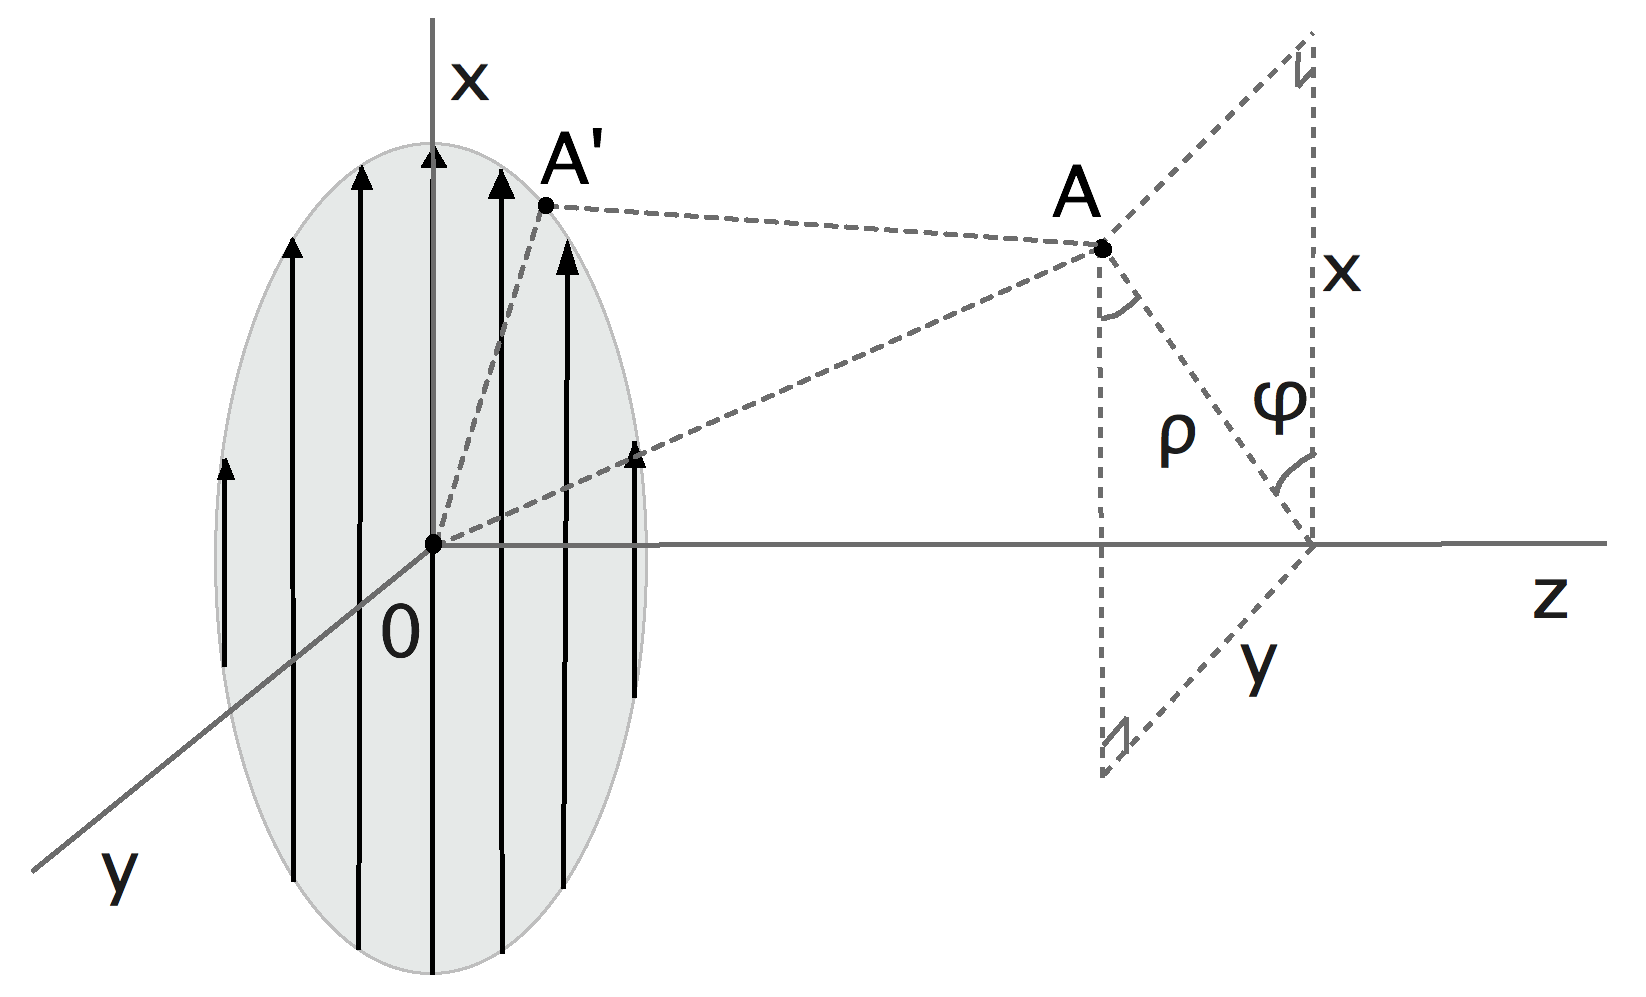
\includegraphics[scale=0.55]{PlaneDisk}
\caption{Геометрія випромінювача} \label{fig:pdisk}
\end{center} \end{figure}
%
\textcolor{lightgray} { \begin{equation*} \begin{aligned}
\begin{cases}
\vect{\rho_0} = \vect{x_0} \cos \varphi + \vect{y_0} \sin \varphi \\
\vect{\varphi_0} = - \vect{x_0} \sin \varphi + \vect{y_0} \cos \varphi
\end{cases} \Rightarrow \mathbf{A} = \left( \begin{array}{cc}
\cos \varphi & \sin \varphi \\
- \sin \varphi & \cos \varphi
\end{array} \right)
\end{aligned} \end{equation*} }
%
\textcolor{lightgray} { \begin{equation*} \begin{aligned}
\vect{j_0} \left( \vect{\rho_0}, \vect{\varphi_0} \right) = 
\mathbf{A} \vect{j_0} \left( \vect{x_0}, \vect{y_0} \right) = \\
= H(t) \delta(z) (  H(\rho) - H(\rho - R) ) 
( \vect{\rho_0} \cos \varphi - \vect{\varphi_0} \sin \varphi )
\end{aligned} \end{equation*} }
%
\begin{equation}
j_m \left( r, t; \nu \right) = \frac{\sqrt{\mu_0}}{2\pi} 
\int \limits_{0}^{2\pi} d \varphi \int \limits_{0}^{\infty} \rho d \rho 
\vect{j_0} \crossprod{ \nabla_\perp \Psi_m^* }{ \vect{z_0} }
\end{equation}
%
\textcolor{lightgray} { \begin{equation*} \begin{aligned}
\crossprod{ \nabla_\perp \Psi_m^* }{ \vect{z_0} } = 
- \sqrt{\nu} e^{-im\varphi} \left( 
\vect{\varphi_0} \frac{J_{m-1} (\nu \rho) - J_{m+1} (\nu \rho)}{2} + 
\right. \\ + \left. i m \vect{\rho_0} \frac{J_m (\nu \rho)}
{\rho \nu} \right) = - \sqrt{\nu} e^{-im\varphi} \left( 
\vect{\varphi_0} \frac{J_{m-1} (\nu \rho) - J_{m+1} (\nu \rho)}{2} + 
\right. \\ + \left. i \vect{\rho_0} \frac{J_{m-1} (\nu \rho) + 
J_{m+1} (\nu \rho)}{2} \right)
\end{aligned} \end{equation*} }
%
\textcolor{lightgray} { \begin{equation*} \begin{aligned}
\vect{j_0} \crossprod{ \nabla_\perp \Psi_m^* }{ \vect{z_0} } = 
- \sqrt{\nu} ( \cos m \varphi - i \sin m \varphi ) 
H(t) \delta(z) ( H(\rho) - H(\rho - R) ) \cdot \\ \cdot \left( 
i \frac{J_{m-1} (\nu \rho) + J_{m+1} (\nu \rho)}{2} \cos \varphi
- \frac{J_{m-1} (\nu \rho) - J_{m+1} (\nu \rho)}{2} \sin \varphi
\right)
\end{aligned} \end{equation*} }
%
\textcolor{red}{ Среда распространения и начальные условия }
%
\textcolor{lightgray} { \begin{equation*} \begin{aligned}
j_m = \frac{\sqrt{\mu_0}}{2\pi} \sqrt{\nu} \delta(z) H(t) \cdot \\
\cdot \Big( \int \limits_{0}^{2\pi} d \varphi \sin \varphi 
( \cos m \varphi - i \sin m \varphi) \int \limits_{0}^{R} 
\frac{J_{m-1} (\nu \rho) - J_{m+1} (\nu \rho)}{2} \rho d \rho - \\
- i \int \limits_{0}^{2\pi} d \varphi \cos \varphi 
( \cos m \varphi - i \sin m \varphi) \int \limits_{0}^{R} 
\frac{J_{m-1} (\nu \rho) + J_{m+1} (\nu \rho)}{2} \rho d \rho \Big)
\end{aligned} \end{equation*} }
%
\textcolor{red} { \begin{equation*} \begin{aligned}
\int \limits_{0}^{2\pi} d \varphi \sin \varphi 
( \cos m \varphi - i \sin m \varphi) = i\pi ( \delta_{m,-1} - \delta_{m,1} )
\end{aligned} \end{equation*} }
%
\textcolor{red} { \begin{equation*} \begin{aligned}
\int \limits_{0}^{2\pi} d \varphi \cos \varphi 
( \cos m \varphi - i \sin m \varphi) = \pi ( \delta_{m,-1} + \delta_{m,1} )
\end{aligned} \end{equation*} }
%
\textcolor{lightgray} { \begin{equation*} \begin{aligned}
j_m = \frac{\sqrt{\mu_0}}{2\pi} \sqrt{\nu} \delta(z) H(t) 
i\pi ( \delta_{m,-1} - \delta_{m,1} ) \int \limits_{0}^{R} 
\frac{J_{m-1} (\nu \rho) - J_{m+1} (\nu \rho)}{2} \rho d \rho - \\
- \frac{\sqrt{\mu_0}}{2\pi} \sqrt{\nu} \delta(z) H(t) 
i\pi ( \delta_{m,-1} + \delta_{m,1} ) \int \limits_{0}^{R} 
\frac{J_{m-1} (\nu \rho) + J_{m+1} (\nu \rho)}{2} \rho d \rho =
\end{aligned} \end{equation*} }
%
\textcolor{lightgray} { \begin{equation*} \begin{aligned}
= i \frac{\sqrt{\mu_0 \nu}}{4} \delta(z) H(t)
\delta_{m,-1} \int \limits_{0}^{R} \left( J_{-2} (\nu \rho) - 
J_0 (\nu \rho) \right) \rho d \rho - \\
- i \frac{\sqrt{\mu_0 \nu}}{4} \delta(z) H(t)
\delta_{m,1} \int \limits_{0}^{R} \left( J_{0} (\nu \rho) - 
J_2 (\nu \rho) \right) \rho d \rho - \\
- i \frac{\sqrt{\mu_0 \nu}}{4} \delta(z) H(t)
\delta_{m,-1} \int \limits_{0}^{R} \left( J_{-2} (\nu \rho) +  
J_0 (\nu \rho) \right) \rho d \rho - \\
- i \frac{\sqrt{\mu_0 \nu}}{4} \delta(z) H(t)
\delta_{m,1} \int \limits_{0}^{R} \left( J_{0} (\nu \rho) +
J_2 (\nu \rho) \right) \rho d \rho =
\end{aligned} \end{equation*} }
%
\textcolor{lightgray} { \begin{equation*} \begin{aligned}
= - i \frac{\sqrt{\mu_0 \nu}}{2} \delta(z) H(t) 
(\delta_{m,1} + \delta_{m,-1}) 
\int \limits_{0}^{R} \left( J_{0} (\nu \rho) + 
J_2 (\nu \rho) \right) \rho d \rho - \\
- i \frac{\sqrt{\mu_0 \nu}}{2} \delta(z) H(t) 
(\delta_{m,1} + \delta_{m,-1}) 
\int \limits_{0}^{R} \left( J_{0} (\nu \rho) -
J_2 (\nu \rho) \right) \rho d \rho = \\
= - i \frac{\sqrt{\mu_0 \nu}}{2} \delta(z) H(t) 
(\delta_{m,1} + \delta_{m,-1}) 
\int \limits_{0}^{R} J_{0} (\nu \rho) \rho d \rho
\end{aligned} \end{equation*} }
%
\textcolor{lightgray} { \begin{equation*} \begin{aligned}
\int \limits_{0}^{R} J_{0} (\nu \rho) \rho d \rho = 
\frac{1}{\nu^2} \int \limits_{0}^{R} J_{0} (\nu \rho) \nu \rho d \nu \rho =
\left. \frac{\rho J_1 (\nu \rho) }{\nu} \right|_{0}^{R} = 
\frac{R J_1 (\nu R)}{\nu}
\end{aligned} \end{equation*} }
%
\begin{equation} 
j_m (z, t; \nu) = - i R A_0 \frac{\sqrt{\mu_0}}{2} \delta(z) H(t) 
\frac{\delta_{m,1} + \delta_{m,-1}}{\sqrt{\nu}} J_1 (\nu R)
\end{equation}

%%%%%%%%%%%%%%%%%%%%%%%%%%%%%%%%%%%%%%%%%%%%%%%%%%%%%%%%%%%%%%%%%%%%%%%%%%%%%%%
\section{Лінійні коефіцієнти}

\begin{equation} \begin{aligned}
V_m^h  = - \mu \partial_{ct} (h_m)
\end{aligned} \end{equation}
%
\begin{equation} \begin{aligned}
I_m^h  = \partial_z (h_m)
\end{aligned} \end{equation}
%
\textcolor{lightgray} { \begin{equation*} \begin{aligned}
- \epsilon \partial_{ct} (V_m^h) - \partial_z I_m^h + \nu^2 h_m = 
\frac{\sqrt{\mu_0}}{2 \pi} \int_0^{2\pi} d \varphi 
\int_0^{\infty} \rho d \rho \crossprod{\vect{z_0}}{\vect{J_\perp}}
\nabla_\perp \Psi_m^* (\nu) 
\end{aligned} \end{equation*} }
%
\textcolor{red} { \begin{equation*} \begin{aligned}
\crossprod{\vect{z_0}}{\vect{J_\perp}} \nabla_\perp \Psi_m^* (\nu) =
\vect{J_\perp} \crossprod{\nabla_\perp \Psi_m^* (\nu)}{\vect{z_0}}
\end{aligned} \end{equation*} }
%
\begin{equation*} \begin{aligned}
\epsilon \partial_{ct} \left( \mu \partial_{ct} h_m \right) -
\mu^{-1} \partial_z \left( \mu  \partial_z h_m \right) + 
\nu^2 h_m = j_m (z,t,\nu) \\
\partial_{ct} =  \frac{1}{c} \partder{}{t}; 
\epsilon = \epsilon (z,t);
\mu = \mu (z,t)
\end{aligned} \end{equation*}
%
\begin{equation} \begin{aligned}
\left( \frac{\sqrt{\epsilon \mu}}{c} \right)^2 
\frac{\partial^2 h_m}{\partial t^2} - 
\frac{\partial^2 h_m}{\partial z^2} + \nu^2 h_m = j_m (z,t,\nu)
\end{aligned} \end{equation}
%
\begin{equation} \begin{aligned}
\mathit{V} = \frac{c}{\sqrt{\epsilon \mu}} 
\end{aligned} \end{equation}
%
\textcolor{red}{Функція Рімана: перевірити принцип причинності}
%
\begin{equation*}
G(t,t',z,z') = \frac{\mathit{V}}{2} H \left( \mathit{V} (t-t') - (z-z') \right)
J_0 \left( \nu \sqrt{\mathit{V}^2 (t-t')^2 - (z-z')^2} \right)
\end{equation*}
%
\begin{equation}
h_m (z, t; \nu) = \iint_S j_m (t',z') G(t,t',z,z') dt' dz'
\end{equation}
%
\textcolor{lightgray} { \begin{equation*} \begin{aligned}
h_m (z, t; \nu) = - i \mathit{V} R \frac{\sqrt{\mu_0}}{4} 
\frac{\delta_{m,1} + \delta_{m,-1}}{\sqrt{\nu}} J_1 (\nu R)
\int \limits_{0}^{\infty} \delta(z) \cdot \\ \cdot
\int \limits_{t - \frac{z}{\mathit{V}}}^{0} 
J_0 \left( \nu \sqrt{\mathit{V}^2 (t-t')^2 - (z-z')^2} \right) dt' dz' = 
i \mathit{V} R \frac{\sqrt{\mu_0}}{4} 
\frac{\delta_{m,1} + \delta_{m,-1}}{\sqrt{\nu}} J_1 (\nu R)
\cdot \\ \cdot \int \limits_{0}^{\infty} \delta(z)
\int \limits_{0}^{t - \frac{z}{\mathit{V}}} 
J_0 \left( \nu \sqrt{\mathit{V}^2 (t-t')^2 - (z-z')^2} \right) dt' dz
\end{aligned} \end{equation*} }
%
\textcolor{lightgray} { \begin{equation*} \begin{aligned}
h_m (z, t; \nu) = i \mathit{V} R \frac{\sqrt{\mu_0}}{4} 
\frac{\delta_{m,1} + \delta_{m,-1}}{\sqrt{\nu}} J_1 (\nu R)
\int \limits_{0}^{t - \frac{z}{\mathit{V}}} 
J_0 \left( \nu \sqrt{\mathit{V}^2 (t-t')^2 - z^2} \right) dt'
\end{aligned} \end{equation*} }
%
\textcolor{red}{Перевірити вірність наступної нотожності
%
\begin{equation}
h_m = \frac{i R A_0}{4} \frac{\delta_{m,1} + \delta_{m,-1}}
{\sqrt{\nu} \sqrt{\epsilon_0 \epsilon \mu}} J_1 (\nu R) 
\int \limits_{0}^{t - \frac{z}{\mathit{V}}} 
J_0 \left( \nu \sqrt{\mathit{V}^2 (t-t')^2 - z^2} \right) dt'
\end{equation} }
%
Для отримання виразу для $ V_m^h $ необовязково брати інткграл в $ h_m $ 
спробуємо спростити вираз скориставшись залкжнісю через похідну по часу.
застосуємо правило інтерування Лейбніца \textcolor{red}{[ПОСИЛАННЯ]}.
%
\begin{equation} \begin{aligned} \label{eq:leibniz_rule}
\partder{}{\theta} \int_{a(\theta)}^{b(\theta)} f(x,\theta) dx = 
\int_{a(\theta)}^{b(\theta)} \partder{f}{\theta} dx + 
f\big( b(\theta), \theta \big) \partder{b}{\theta} -
f\big( a(\theta), \theta \big) \partder{a}{\theta}
\end{aligned} \end{equation}
%
В очевидь, знадобиться похідна від функції Бесселя складного аргументу.
%
\textcolor{lightgray} { \begin{equation*} \begin{aligned}
\partder{}{t} J_0 \left( \nu \sqrt{v^2 (t-t')^2 - z} \right) = 
- \nu J_1 \left( \nu \sqrt{v^2 (t-t')^2 - z} \right) 
\partder{}{t} \sqrt{v^2 (t-t')^2 - z} = \\
-  J_1 \left( \nu \sqrt{v^2 (t-t')^2 - z} \right)
\frac{2 \nu v^2 (t-t')}{2 \sqrt{v^2 (t-t')^2 - z}} = - \nu v^2 (t-t') 
\frac{J_1 \left( \nu \sqrt{v^2 (t-t')^2 - z} \right)}
     {\sqrt{v^2 (t-t')^2 - z}}
\end{aligned} \end{equation*} }
%
\begin{equation*} \begin{aligned}
\partder{}{t} J_0 \left( \nu \sqrt{v^2 (t-t')^2 - z} \right) = - \nu v^2 (t-t') 
\frac{J_1 \left( \nu \sqrt{v^2 (t-t')^2 - z} \right)}{\sqrt{v^2 (t-t')^2 - z}}
\end{aligned} \end{equation*}
%
Відразу помічаємо, що
%
\begin{equation} \begin{aligned} \label{eq:j0_hard_perp_t}
\partder{}{t'} J_0 \left( \nu \sqrt{v^2 (t-t')^2 - z} \right) =
- \partder{}{t} J_0 \left( \nu \sqrt{v^2 (t-t')^2 - z} \right) 
\end{aligned} \end{equation}
%
Тепер застосуємо \eqref{eq:leibniz_rule} з \eqref{eq:j0_hard_perp_t} та 
отримаємо спрощення - один иінтегралів зникає
%
\textcolor{lightgray} { \begin{equation*} \begin{aligned}
\partder{}{t} \int \limits_{0}^{t - \frac{z}{v}} 
J_0 \left( \nu \sqrt{v^2 (t-t')^2 - z^2} \right) dt' = \\
= \int \limits_{0}^{t - \frac{z}{v}} 
\partder{}{t} J_0 \left( \nu \sqrt{v^2 (t-t')^2 - z^2} \right) dt' +
J_0 (0) - 0 \cdot \left( \nu \sqrt{v^2 (t-t')^2 - z^2} \right) = \\
= - \int \limits_{0}^{t - \frac{z}{v}} 
\partder{}{t'} J_0 \left( \nu \sqrt{v^2 (t-t')^2 - z^2} \right) dt' + 1 =
- \Big. J_0 \left( \nu \sqrt{v^2 (t-t')^2 - z^2} \right) \Big|_{0}^{t - \frac{z}{v}} + 1 = \\
- J_0 \left( \nu \sqrt{z^2 - z^2} \right) + J_0 \left( \nu \sqrt{v^2 t^2 - z^2} \right) + 1 = 
J_0 \left( \nu \sqrt{v^2 t^2 - z^2} \right)
\end{aligned} \end{equation*} }
%
\begin{equation} \begin{aligned}
\partder{}{t} \int \limits_{0}^{t - \frac{z}{v}} 
J_0 \left( \nu \sqrt{v^2 (t-t')^2 - z^2} \right) dt' =
J_0 \left( \nu \sqrt{v^2 t^2 - z^2} \right)
\end{aligned} \end{equation}
%
\textcolor{lightgray} { \begin{equation*} \begin{aligned}
V_m^h = - \frac{\mu}{c} \partder{h_m}{t} = 
\sqrt{\mu_0} \sqrt{\frac{\mu}{\epsilon}} \frac{iR A_0}{4} 
\frac{\delta_{m,1} + \delta_{m,-1}}{\sqrt{\nu}} J_1 (\nu R)
J_0 \left( \nu \sqrt{\mathit{V}^2 t^2 - z^2} \right)
\end{aligned} \end{equation*} }
%
Тепер можемо записати формулу для коефійієнту $ V_m^h $
%
\begin{equation}
V_m^h (z, t; \nu) = - \frac{iR A_0}{4} \sqrt{\frac{\mu_0 \mu}{\epsilon}} 
\frac{\delta_{m,1} + \delta_{m,-1}}{\sqrt{\nu}} J_1 (\nu R)
J_0 \left( \nu \sqrt{\mathit{V}^2 t^2 - z^2} \right)
\end{equation}
%
\textcolor{lightgray} { \begin{equation*} \begin{aligned}
\int \limits_{0}^{t - \frac{z}{\mathit{V}}} 
J_0 \left( \nu \sqrt{\mathit{V}^2 (t-t')^2 - z^2} 
\right) dt' = \left[ \begin{array}{cc} 
\nu \mathit{V} (t-t') = s & t' = t - \frac{ds}{\nu \mathit{V}} \\
dt' = -\frac{ds}{\nu \mathit{V}} & \\
s(0) = \nu \mathit{V} t & s \left( t - \frac{z}{\mathit{V}} \right) = \nu z
\end{array} \right] = \\ = - \frac{1}{\nu \mathit{V}} 
\int_{\nu \mathit{V} t}^{\nu z} ds 
J_0 (\sqrt{s^2 - \nu^2 z^2}) = \frac{1}{\nu \mathit{V}} 
\int_{\nu z}^{\nu \mathit{V} t} ds
J_0 (\sqrt{s^2 - \nu^2 z^2})
\end{aligned} \end{equation*} }
%
\textcolor{lightgray} { \begin{equation*} \begin{aligned}
\int_{\nu z}^{\nu \mathit{V} t} ds e^{-i0s} J_0 (\sqrt{s^2 - \nu^2 z^2}) = \\ 
= \frac{1}{i} (U_1[W_+,Z] + i U_2[W_+,Z] - U_1[W_-,Z] - i U_2[W_-,Z]) = \\
= \frac{1}{i} (-U_1[W_-,Z] + i U_2[W_+,Z] - U_1[W_-,Z] - i U_2[W_+,Z]) = \\
= \left[ \begin{array}{c} W_\pm = \pm i (\nu \mathit{V} t - \nu z) \\
Z = \sqrt{\nu^2 \mathit{V}^2 t^2 - \nu^2 z^2} \end{array} \right] = 
2i U_1 \left[ -i \nu (\mathit{V}t-z), \nu \sqrt{\mathit{V}^2 t^2-z^2} \right]
\end{aligned} \end{equation*} }
%
\textcolor{lightgray} { \begin{equation*} \begin{aligned}
\int \limits_{0}^{t - \frac{z}{\mathit{V}}} 
J_0 \left( \nu \sqrt{\mathit{V}^2 (t-t')^2 - z^2} 
\right) dt' = \frac{2i}{\nu \mathit{V}} U_1 
\left[ -i \nu (\mathit{V}t-z), \nu \sqrt{\mathit{V}^2t^2-z^2} \right]
\end{aligned} \end{equation*} }
%
\textcolor{lightgray} { \begin{equation*} \begin{aligned}
h_m (z, t; \nu) = \mathit{V} \sqrt{\mu_0} \frac{iR A_0}{4} 
\frac{\delta_{m,1} + \delta_{m,-1}} {\sqrt{\nu}} J_1 (\nu R) 
\frac{2i}{\nu \mathit{V}} U_1 \left[ W_-, Z \right]
\end{aligned} \end{equation*} }
%
\begin{equation}
h_m (z, t; \nu) = - \sqrt{\mu_0} \frac{R A_0}{2} 
\frac{\delta_{m,1} + \delta_{m,-1}}
{\nu^{3/2}} J_1 (\nu R) U_1 \left[ W_-, Z \right]
\end{equation}
%
\textcolor{lightgray} { \begin{equation*} \begin{aligned}
I_{m}^{h} = \partder{h_m}{z} = 
- \sqrt{\mu_0} \frac{R A_0}{2} 
\frac{\delta_{m,1} + \delta_{m,-1}}
{\nu^{3/2}} J_1 (\nu R) \partder{}{z} U_1 [ W_-, Z ]
\end{aligned} \end{equation*} }
%
\textcolor{lightgray} { \begin{equation*} \begin{aligned}
\begin{array}{lcr}
\derivat{W_-}{z} = i \nu & &
\derivat{Z}{z} = \frac{\nu}{2 \sqrt{\mathit{V}^2 t^2 - z^2}} (-2z) = 
- \frac{\nu z}{\sqrt{\mathit{V}^2 t^2 - z^2}} \\
\end{array}
\end{aligned} \end{equation*} }
%
\textcolor{lightgray} { \begin{equation*} \begin{aligned}
\left( \frac{Z}{W} \right)^2 = 
\left( - \frac{ \sqrt{\mathit{V}^2 t^2-z^2}}{i(\mathit{V} t-z)} \right)^2 =
\left( \frac{ i \sqrt{\mathit{V}^2 t^2-z^2}}{\mathit{V}t-z} \right)^2 =
- \frac{\mathit{V}^2 t^2-z^2}{(\mathit{V} t-z)^2} = 
- \frac{\mathit{V}t+z}{\mathit{V}t-z}
\end{aligned} \end{equation*} }
%
\textcolor{lightgray} { \begin{equation*} 
\partder{}{Z} U_n (W,Z) = - \frac{Z}{W} U_{n+1} (W,Z)
\end{equation*} }
%
\textcolor{lightgray} { \begin{equation*}
2 \partder{}{W} U_n (W,Z) = U_{n-1} (W,Z) + 
\left( \frac{Z}{W} \right)^2 U_{n+1} (W,Z)
\end{equation*} }
%
\textcolor{lightgray} { \begin{equation*} \begin{aligned}
\partder{}{z} U_1 \left[ -i \nu (ct-z), \nu \sqrt{c^2t^2-z^2} \right] =
\partder{}{z} U_1[W,Z] = \partder{U_1}{W} \derivat{W}{z} + 
\partder{U_1}{Z} \derivat{Z}{z} = \\
= \frac{i \nu}{2} \left( U_0 - \frac{ct+z}{ct-z} U_2 \right) -
\frac{\nu z}{\sqrt{c^2t^2 - z^2}} 
\left( - \frac{i \sqrt{c^2t^2-z^2}}{ct-z} \right) U_2 = \\
= \frac{i \nu}{2} U_0 - \frac{i \nu}{2} \frac{ct+z}{ct-z} U_2 +
\frac{i \nu z}{ct-z} U_2 = \\ = \frac{i \nu}{2} U_0 - \frac{i \nu}{2} U_2
\left( \frac{ct}{ct-z} + \frac{z}{ct-z} - \frac{2z}{ct-z} \right) = 
\frac{i \nu}{2} (U_0[W_-,Z] - U_2[W_-,Z])
\end{aligned} \end{equation*} }
%
\begin{equation}
I_{m}^{h} = - \sqrt{\mu_0} \frac{iR A_0}{4} 
\frac{\delta_{m,1} + \delta_{m,-1}}{\sqrt{\nu}} 
J_1 (\nu R) \left( U_0 [ W_-, Z ] - U_2 [ W_-, Z ] \right)
\end{equation}

%%%%%%%%%%%%%%%%%%%%%%%%%%%%%%%%%%%%%%%%%%%%%%%%%%%%%%%%%%%%%%%%%%%%%%%%%%%%%%%
\section{Лінійне поле}

\textcolor{lightgray} { \begin{equation*} \begin{aligned}
\vect{E_\perp} = \frac{1}{\sqrt{\epsilon_0}} \left( 
\sum \limits_{m=-\infty}^{\infty} \int \limits_{0}^{\infty} 
d \nu V_m^h \crossprod{ \nabla_\perp \Psi_m }{ \vect{z_0} } +
\sum \limits_{n=-\infty}^{\infty} \int \limits_{0}^{\infty}
d \chi V_n^e \nabla_\perp \Phi_n \right)
\end{aligned} \end{equation*} }
%
\textcolor{lightgray} { \begin{equation*} \begin{aligned}
\crossprod{ \nabla_\perp \Psi_m }{ \vect{z_0} } = 
- e^{im\varphi} \left( \vect{\varphi_0} \sqrt{\nu} 
\frac{J_{m-1} (\nu \rho) - J_{m+1} (\nu \rho)}{2} - 
i m \vect{\rho_0} \frac{J_m (\nu \rho)}{ \rho \sqrt{\nu}} \right)
\end{aligned} \end{equation*} }
%
\textcolor{lightgray} { \begin{equation*} \begin{aligned}
\vect{E_\perp} = \frac{1}{\sqrt{\epsilon_0}} \int_{0}^{\infty} 
V_{-1}^h \crossprod{ \nabla_\perp \Psi_{-1}  }{ \vect{z_0} } +
\frac{1}{\sqrt{\epsilon_0}} \int \limits_{0}^{\infty} 
V_{1}^h \crossprod{ \nabla_\perp \Psi_{1} }{ \vect{z_0} } = \\
= \frac{i R A_0}{4} \sqrt{\frac{\mu_0 \mu}{\epsilon_0 \epsilon}} 
e^{- i \varphi} \int_{0}^{\infty} \frac{J_1 (\nu R)}{\sqrt{\nu}} 
J_0 \left( \nu \sqrt{c^2 t^2 - z^2} \right) \cdot \\
\cdot \left( \vect{\varphi_0} \sqrt{\nu} 
\frac{J_2 (\nu \rho) - J_0 (\nu \rho)}{2} +
i \vect{\rho_0} \frac{J_1 (\nu \rho)}{ \rho \sqrt{\nu}} \right) - \\
+ \frac{i R A_0}{4} \sqrt{\frac{\mu_0 \mu}{\epsilon_0 \epsilon}}
e^{i \varphi} \int \limits_{0}^{\infty} \frac{J_1 (\nu R)}{ \sqrt{\nu}}
J_0 \left( \nu \sqrt{c^2 t^2 - z^2} \right) \cdot \\
\cdot \left( \vect{\varphi_0} \sqrt{\nu}
\frac{J_0 (\nu \rho) - J_2 (\nu \rho)}{2} - 
i \vect{\rho_0} \frac{J_1 (\nu \rho)}{ \rho \sqrt{\nu}} \right)
\end{aligned} \end{equation*} }
%
\textcolor{lightgray} { \begin{equation*} \begin{aligned}
E_\varphi = \frac{i R A_0}{8} \sqrt{\frac{\mu_0 \mu}{\epsilon_0 \epsilon}} 
e^{-i \varphi} \int \limits_{0}^{\infty} J_1 (\nu R)
J_0 \left( \nu \sqrt{c^2 t^2 - z^2} \right)
\left( J_2 (\nu \rho) - J_0 (\nu \rho) \right) + \\
+ \frac{i R A_0}{8} \sqrt{\frac{\mu_0 \mu}{\epsilon_0 \epsilon}} 
e^{i \varphi} \int \limits_{0}^{\infty} J_1 (\nu R)
J_0 \left( \nu \sqrt{c^2 t^2 - z^2} \right)
\left( J_0 (\nu \rho) - J_2 (\nu \rho) \right) = \\
= \frac{i R A_0}{4} \sqrt{\frac{\mu_0 \mu}{\epsilon_0 \epsilon}}
\frac{e^{i \varphi} - e^{-i \varphi} }{2} \int \limits_{0}^{\infty} 
J_1 (\nu R) J_0 \left( \nu \sqrt{c^2 t^2 - z^2} \right) 
\left( J_0 (\nu \rho) - J_2 (\nu \rho) \right) =
\end{aligned} \end{equation*} }
%
\textcolor{lightgray} { \begin{equation*} \begin{aligned}
= \frac{R A_0}{4} \sqrt{\frac{\mu_0 \mu}{\epsilon_0 \epsilon}} 
\frac{e^{i \varphi} - e^{-i \varphi} }{2i} \int \limits_{0}^{\infty} 
J_1 (\nu R) J_0 \left( \nu \sqrt{c^2 t^2 - z^2} \right) 
\left( J_2 (\nu \rho) - J_0 (\nu \rho) \right) = \\
= \frac{R A_0}{4} \sqrt{\frac{\mu_0 \mu}{\epsilon_0 \epsilon}} \sin \varphi 
\int \limits_{0}^{\infty} J_1 (\nu R) 
J_0 \left( \nu \sqrt{c^2 t^2 - z^2} \right) 
\left( J_2 (\nu \rho) - J_0 (\nu \rho) \right)
\end{aligned} \end{equation*} }
%
\textcolor{lightgray} { \begin{equation*} \begin{aligned}
J_2 (\nu \rho) - J_0 (\nu \rho) = \frac{2}{\nu \rho} J_1 (\nu \rho) - 
2 J_0 (\nu \rho)
\end{aligned} \end{equation*} }
%
\textcolor{lightgray} { \begin{equation*} \begin{aligned}
E_\varphi = \frac{R A_0}{2} \sqrt{\frac{\mu_0 \mu}{\epsilon_0 \epsilon}}
\sin \varphi \int \limits_{0}^{\infty} J_1 (\nu R) 
J_0 \left( \nu \sqrt{c^2 t^2 - z^2} \right) 
\left( \frac{J_1 (\nu \rho)}{\nu \rho} - J_0 (\nu \rho) \right)
\end{aligned} \end{equation*} }
%
\textcolor{lightgray} { \begin{equation*} \begin{aligned}
E_\rho = \frac{i R A_0}{4} \sqrt{\frac{\mu_0 \mu}{\epsilon_0 \epsilon}}  
e^{- i \varphi} \int \limits_{0}^{\infty} \frac{J_1 (\nu R)}{\sqrt{\nu}} 
J_0 \left( \nu \sqrt{c^2 t^2 - z^2} \right) 
\left( - i \frac{J_1 (\nu \rho)}{\rho \sqrt{\nu}} \right) + \\
+ \mu \frac{i R A_0}{4} \sqrt{\frac{\mu_0}{\epsilon_0}}  e^{i \varphi}
\int \limits_{0}^{\infty} \frac{J_1 (\nu R)}{\sqrt{\nu}}
J_0 \left( \nu \sqrt{c^2 t^2 - z^2} \right) 
\left( - i \frac{J_1 (\nu \rho)}{ \rho \sqrt{\nu}} \right) = \\
= \mu \frac{R A_0}{2} \sqrt{\frac{\mu_0 \mu}{\epsilon_0 \epsilon}} 
\frac{e^{i \varphi} + e^{-i \varphi}}{2}
\int \limits_{0}^{\infty} \frac{J_1 (\nu R)}{\sqrt{\nu}}
J_0 \left( \nu \sqrt{c^2 t^2 - z^2} \right) 
\frac{J_1 (\nu \rho)}{ \rho \sqrt{\nu}} = \\
= \mu \frac{R A_0}{2} \sqrt{\frac{\mu_0 \mu}{\epsilon_0 \epsilon}} 
\cos \varphi \int \limits_{0}^{\infty} \frac{d \rho}{\nu \rho} 
J_1 (\nu \rho) J_1 (\nu R) J_0 \left( \nu \sqrt{c^2 t^2 - z^2} \right)
\end{aligned} \end{equation*} }
%
\begin{equation} \label{eq:linear_e_cyl}
\vect{E} \left( r, t \right) = \frac{A_0}{2} 
\sqrt{\frac{\mu_0 \mu}{\epsilon_0 \epsilon}}
\Big( \vect{\rho_0} I_1 \cos \varphi - 
\vect{ \varphi_0 } \left( I_2 - I_1 \right) \sin \varphi \Big)
\end{equation}
%
\begin{equation*}
I_1 = R \int \limits_{0}^{\infty} \frac{d \nu}{\nu \rho} J_1 (\nu \rho) 
J_1 (\nu R) J_0 \left( \nu \sqrt{\frac{c^2 t^2}{\epsilon \mu} - z^2} \right)
\end{equation*}
%
\begin{equation*}
I_2 = R \int_{0}^{\infty} d \nu J_1 (\nu R) 
J_0 (\nu \rho) J_0 \left( \nu \sqrt{\frac{c^2 t^2}{\epsilon \mu} - z^2} \right)
\end{equation*}
%
\textcolor{red} { Правильній перехід до декартових векторних кординат? } 
%
\textcolor{lightgray} { \begin{equation*} \begin{aligned}
\mathbf{A} = \left( \begin{array}{cc}
\cos \varphi & \sin \varphi \\
- \sin \varphi & \cos \varphi
\end{array} \right) \begin{array}{ccc}
	& \det A = 1 		&	\\
	& A^{-1} = A^{T}	&
\end{array} 
\mathbf{A^{-1}} = \left( \begin{array}{cc}
\cos \varphi & - \sin \varphi \\
\sin \varphi & \cos \varphi
\end{array} \right) 
\end{aligned} \end{equation*} }
%
\begin{figure}[h] \begin{center}
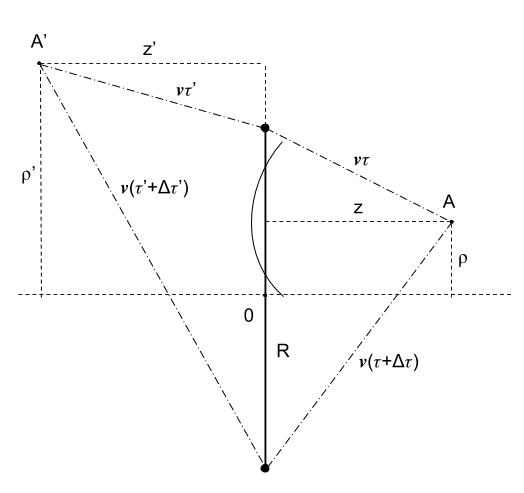
\includegraphics[scale=0.6]{PartialRadiation}
\caption{Фізичний зміст областей випромінювання} \label{fig:part_rad}
\end{center} \end{figure}
%
\textcolor{lightgray} { \begin{equation*} \begin{aligned}
\vect{E} = 
\mathbf{A^{-1}} \vect{E} \left( \vect{\rho_0}, \vect{\varphi_0} \right) = 
\frac{A_0}{2} \sqrt{\frac{\mu_0 \mu}{\epsilon_0 \epsilon}}
\left( \begin{array}{cc} \cos \varphi & - \sin \varphi \\
\sin \varphi & \cos \varphi \end{array} \right)
\left( \begin{array}{c} I_1 \cos \varphi \\
- (I_2 - I_1) \sin \varphi \end{array} \right) = \\
= \frac{A_0}{2} \sqrt{\frac{\mu_0 \mu}{\epsilon_0 \epsilon}}
\left( \begin{array}{c} I_1 \cos^2 \varphi + (I_2 - I_1) \sin^2 \varphi \\
I_1 \sin \varphi \cos \varphi - (I_2 - I_1) 
\sin \varphi \cos \varphi \end{array} \right)
\end{aligned} \end{equation*} }
%
\begin{equation*} \begin{aligned}
\vect{E} \left( \vect{x_0}, \vect{y_0} \right) = \frac{A_0}{2} 
\sqrt{\frac{\mu_0 \mu}{\epsilon_0 \epsilon}} \left( \begin{array}{c} 
I_1 \cos^2 \varphi + (I_2 - I_1) \sin^2 \varphi \\
I_1 \sin \varphi \cos \varphi - (I_2 - I_1) 
\sin \varphi \cos \varphi \end{array} \right)
\end{aligned} \end{equation*}
%
Для зони $ S_3 $ тільки $ E_x $ компонента електричного поля не дорівнює
нулю. Окрім того амплітуда $ E_x $ постійна для всіх подій з облсті $ S_3 $.
%
\begin{equation*} \begin{aligned}
\vect{E} = \vect{x_0} \frac{A_0}{4} 
\sqrt{\frac{\mu_0 \mu}{\epsilon_0 \epsilon}}
\end{aligned} \end{equation*}
%
\begin{figure}[h] \begin{center}
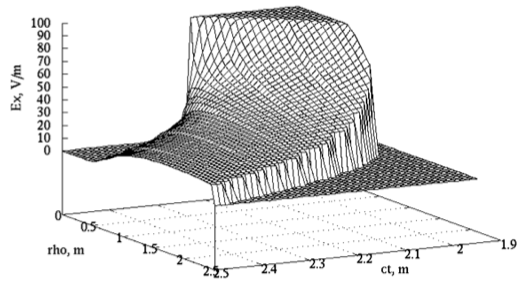
\includegraphics[scale=0.6]{MissileEffect}
\caption{Ефект електромагнітного снаряду ($ z = 2 $ м)} \label{fig:emp_rho}
\end{center} \end{figure}
%
Такий ефект носить назву електромагнітного знаряду. Хоча поле в явному
виді не залежить від точки спостереження, залежність присутня в визначенні 
зон випромінювання поля плаского диску. Користуючить ними можна вирахувати 
тривалість ефекту.
%
\begin{equation*} \begin{aligned}
\frac{c \tau}{\sqrt{\epsilon \mu}} = \sqrt{R^2+z^2} - z.
\end{aligned} \end{equation*}
%
При $ R = 1 $ можна ввести апроксимацію цієї формули, як  
%
\begin{equation*} \begin{aligned}
\frac{c \tau}{\sqrt{\epsilon \mu}} \left( z \gg 2R \right) \approx 
\begin{cases}
\frac{2R}{z} , R \geq 1 \\
\frac{R^2}{2z} , R \leq 1
\end{cases}
\end{aligned} \end{equation*}
%
\begin{figure}[h] \begin{center}
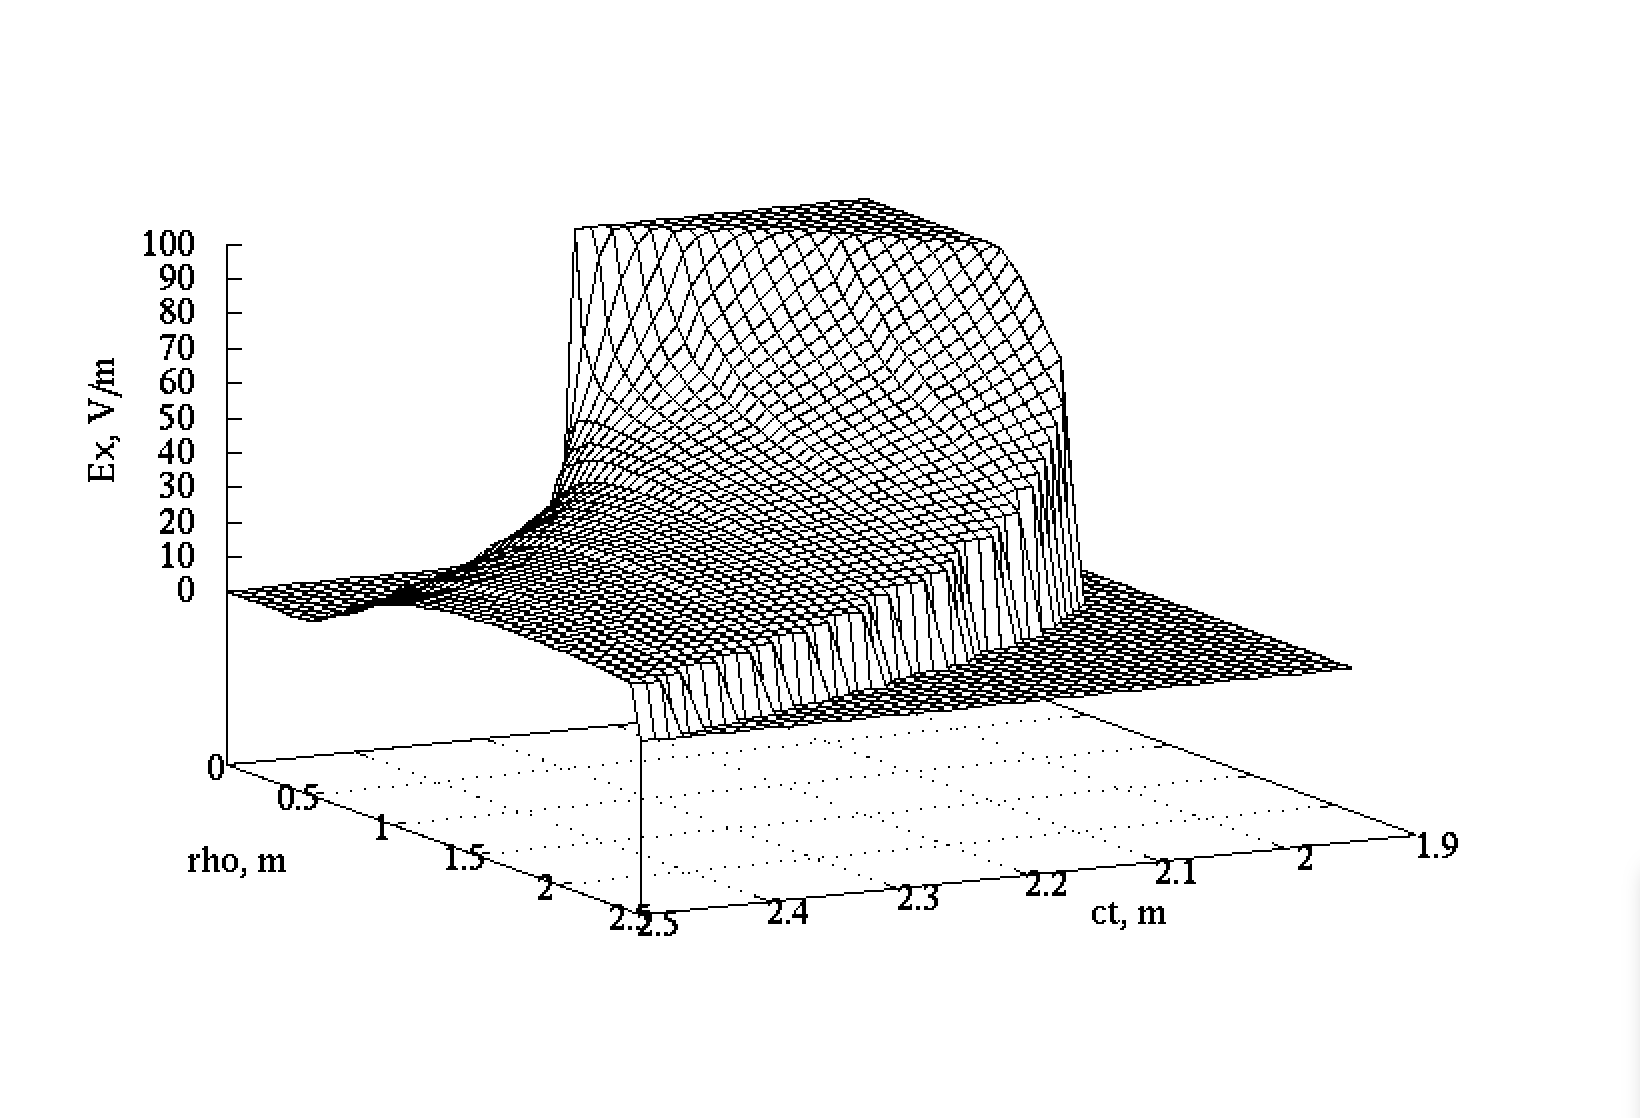
\includegraphics[scale=0.6]{TransientEffect}
\caption{Ефект електромагнітного снаряду ($ \rho = 0.2 $ м)} \label{fig:emp_z}
\end{center} \end{figure}
%
\begin{figure}[h] \begin{center}
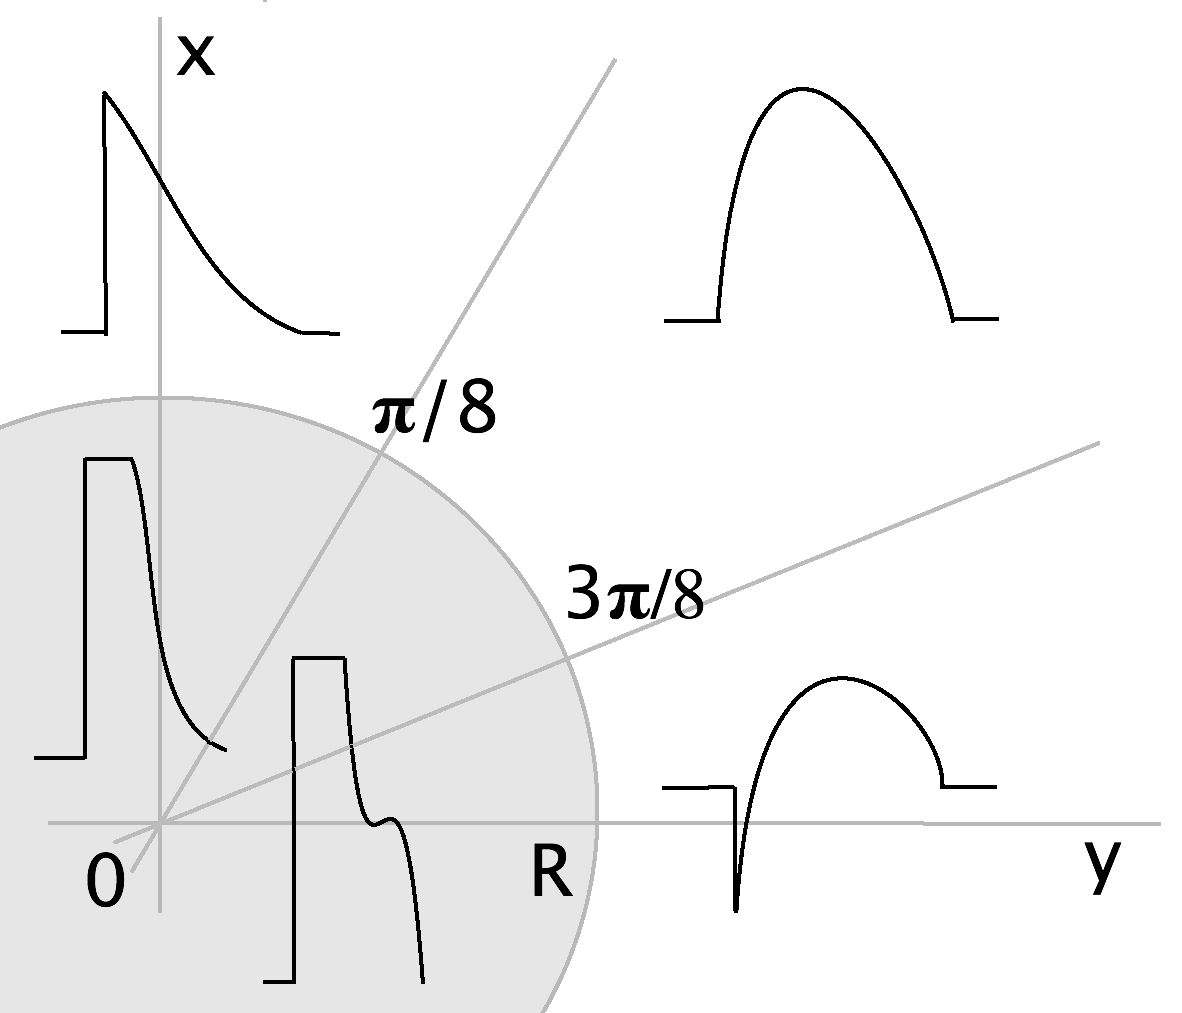
\includegraphics[scale=0.7]{LinearPulsShape}
\caption{Кутова залежнысть формы імпульсу ($ \rho = R/2 .. 2R $ м)} 
\label{fig:emp_shape}
\end{center} \end{figure}
%
\textcolor{lightgray} { \begin{equation*} \begin{aligned}
\vect{H_\perp} = \frac{1}{\sqrt{\mu_0}} \left( 
\sum \limits_{m=-\infty}^{\infty} \int \limits_{0}^{\infty} d \nu
I_m^h \nabla_\perp \Psi_m + \sum \limits_{n=-\infty}^{\infty}
\int \limits_{0}^{\infty} d \chi I_n^e 
\crossprod{\vect{z_0}}{\nabla_\perp \Phi_n} \right)
\end{aligned} \end{equation*} }
%
\textcolor{lightgray} { \begin{equation*} \begin{aligned}
\nabla_\perp \Psi_m = e^{i m \varphi} \left( \vect{\rho_0} 
\sqrt{\nu} \frac{ J_{m-1}(\nu \rho) - J_{m+1}(\nu \rho) }{2} +
i m \vect{\varphi_0} \frac{J_m(\nu \rho)}{\sqrt{\nu} \rho} \right)
\end{aligned} \end{equation*} }
%
\textcolor{lightgray} { \begin{equation*} \begin{aligned}
\vect{H_\perp} = \frac{1}{\sqrt{\mu_0}} \left( 
\int \limits_{0}^{\infty} d \nu I_{-1}^h \nabla_\perp \Psi_{-1} +
\int \limits_{0}^{\infty} d \nu I_1^h \nabla_\perp \Psi_1 \right) = \\
= - \frac{A_0}{\sqrt{\mu_0}} \int \limits_{0}^{\infty} d \nu
\sqrt{\mu_0} \frac{iR}{4} J_1 (\nu R)
\frac{ U_0 [ W_-, Z ] - U_2 [ W_-, Z ] }{\sqrt{\nu}}  
e^{- i \varphi} \cdot \\ \cdot \left( \vect{\rho_0} 
\sqrt{\nu} \frac{ J_{2}(\nu \rho) - J_{0}(\nu \rho) }{2} +
i \vect{\varphi_0} \frac{J_1(\nu \rho)}{\sqrt{\nu} \rho} \right) -
\frac{A_0}{\sqrt{\mu_0}} \int \limits_{0}^{\infty} d \nu 
\sqrt{\mu_0} \frac{iR}{4} J_1 (\nu R) \cdot \\
\cdot \frac{ U_0 [ W_-, Z ] - U_2 [ W_-, Z ] }{\sqrt{\nu}} 
e^{i \varphi} \left( \vect{\rho_0} 
\sqrt{\nu} \frac{ J_{0}(\nu \rho) - J_{2}(\nu \rho) }{2} +
i \vect{\varphi_0} \frac{J_1(\nu \rho)}{\sqrt{\nu} \rho} \right)
\end{aligned} \end{equation*} }
%
\textcolor{lightgray} { \begin{equation*} \begin{aligned}
H_\varphi = \frac{R A_0}{4} 
\frac{e^{i \varphi} + e^{- i \varphi}}{\rho} \int \limits_{0}^{\infty} 
\frac{d\nu}{\nu} (U_0[ W_-, Z ] - U_2[ W_-, Z ]) J_1(\nu R) J_1(\nu \rho) = \\
= \frac{R}{2} \cos \varphi \int \limits_{0}^{\infty}
\frac{d\nu}{\nu \rho} (U_0[ W_-, Z ] - U_2[ W_-, Z ]) 
J_1(\nu R) J_1(\nu \rho)
\end{aligned} \end{equation*} }
%
\textcolor{lightgray} { \begin{equation*} \begin{aligned}
H_\rho = \frac{R A_0}{4} \frac{e^{i \varphi} - e^{- i \varphi}}{2i}
\int \limits_{0}^{\infty} d \nu (J_{0}(\nu \rho) - J_{2}(\nu \rho))
J_1(\nu R) (U_0[ W_-, Z ] - U_2[ W_-, Z ]) = \\
= \frac{R}{2} \sin \varphi \int \limits_{0}^{\infty} d \nu 
(J_0(\nu \rho) - \frac{J_1(\nu \rho)}{\nu \rho})
J_1(\nu R) (U_0[ W_-, Z ] - U_2[ W_-, Z ]) = \\
\end{aligned} \end{equation*} }
%
\textcolor{lightgray} { \begin{equation*} \begin{aligned}
\vect{H_\perp} \left( r, t \right) = \frac{A_0}{2} \left( 
\vect{\rho_0} \left( I_4 - I_3 \right) \sin \varphi +
\vect{\varphi_0} I_3 \cos \varphi  \right)
\end{aligned} \end{equation*} }
%
\textcolor{lightgray} { \begin{equation*} \begin{aligned}
H_z (r,t) = \frac{1}{\sqrt{\mu_0}} \sum \limits_{m=-\infty}^{\infty}
\int \limits_0^\infty \nu^2 d \nu h_m \Psi_m
\end{aligned} \end{equation*} }
%
\textcolor{lightgray} { \begin{equation*} \begin{aligned}
\Psi_m (\nu) = \frac{J_m(\nu \rho)}{\sqrt{\nu}} e^{im \varphi} 
\end{aligned} \end{equation*} }
%
\textcolor{lightgray} { \begin{equation*} \begin{aligned}
H_z (r,t) = 
\frac{1}{\sqrt{\mu_0}} \int \limits_0^\infty \nu^2 d \nu h_{1} \Psi_{1} +
\frac{1}{\sqrt{\mu_0}} \int \limits_0^\infty \nu^2 d \nu h_{-1} \Psi_{-1}
\end{aligned} \end{equation*} }
%
\textcolor{lightgray} { \begin{equation*} \begin{aligned}
H_z (r,t) = R A_0 \frac{e^{im \varphi}-e^{-im \varphi}}{2} \int_0^\infty 
d \nu J_1(\nu \rho) J_1 (\nu R)
U_1 \left[ -i \nu (ct-z), \nu \sqrt{c^2t^2-z^2} \right]
\end{aligned} \end{equation*} }
%
\textcolor{lightgray} { \begin{equation*} \begin{aligned}
H_z (r,t) = - R A_0 \sin \varphi \int_0^\infty 
d \nu J_1(\nu \rho) J_1 (\nu R) U_1 [ W_-, Z ] = \\
= - i R A_0 \sin \varphi \int_{0}^{\infty} J_1 \left( \nu R \right)
J_1 \left( \nu \rho \right) U_1 [ W_-, Z ]
\end{aligned} \end{equation*} }
%
\textcolor{lightgray} { \begin{equation*} \begin{aligned}
H_z \left( r, t \right) = - A_0 I_5 \sin \varphi
\end{aligned} \end{equation*} }
%
\begin{equation} \label{eq:linear_h_cyl}
\vect{H} (r, t) = \frac{A_0}{2} \Big( 
\vect{\rho_0} \left( I_4 - I_3 \right) \sin \varphi +
\vect{\varphi_0} I_3 \cos \varphi -
2 \vect{z_0} I_5 \sin \varphi \Big)
\end{equation}
%
\begin{equation*}
I_3 = R \int \limits_{0}^{\infty}
\frac{d\nu}{\nu \rho} J_1(\nu R) J_1(\nu \rho)
\Big( U_0[ W_-, Z ] - U_2[ W_-, Z ] \Big) 
\end{equation*}
%
\begin{equation*}
I_4 = R \int \limits_{0}^{\infty} d\nu J_1(\nu R) J_0(\nu \rho)
\Big( U_0[ W_-, Z ] - U_2[ W_-, Z ] \Big) 
\end{equation*}
%
\begin{equation*}
I_5 = i R \int \limits_0^\infty 
d \nu J_1(\nu \rho) J_1 (\nu R)
U_1 \left[ -i \nu \left( \frac{ct}{\sqrt{\epsilon \mu}} - z \right), 
\nu \sqrt{\frac{c^2t^2}{\epsilon \mu}-z^2} \right]
\end{equation*}
%
\begin{figure}[h] \begin{center}
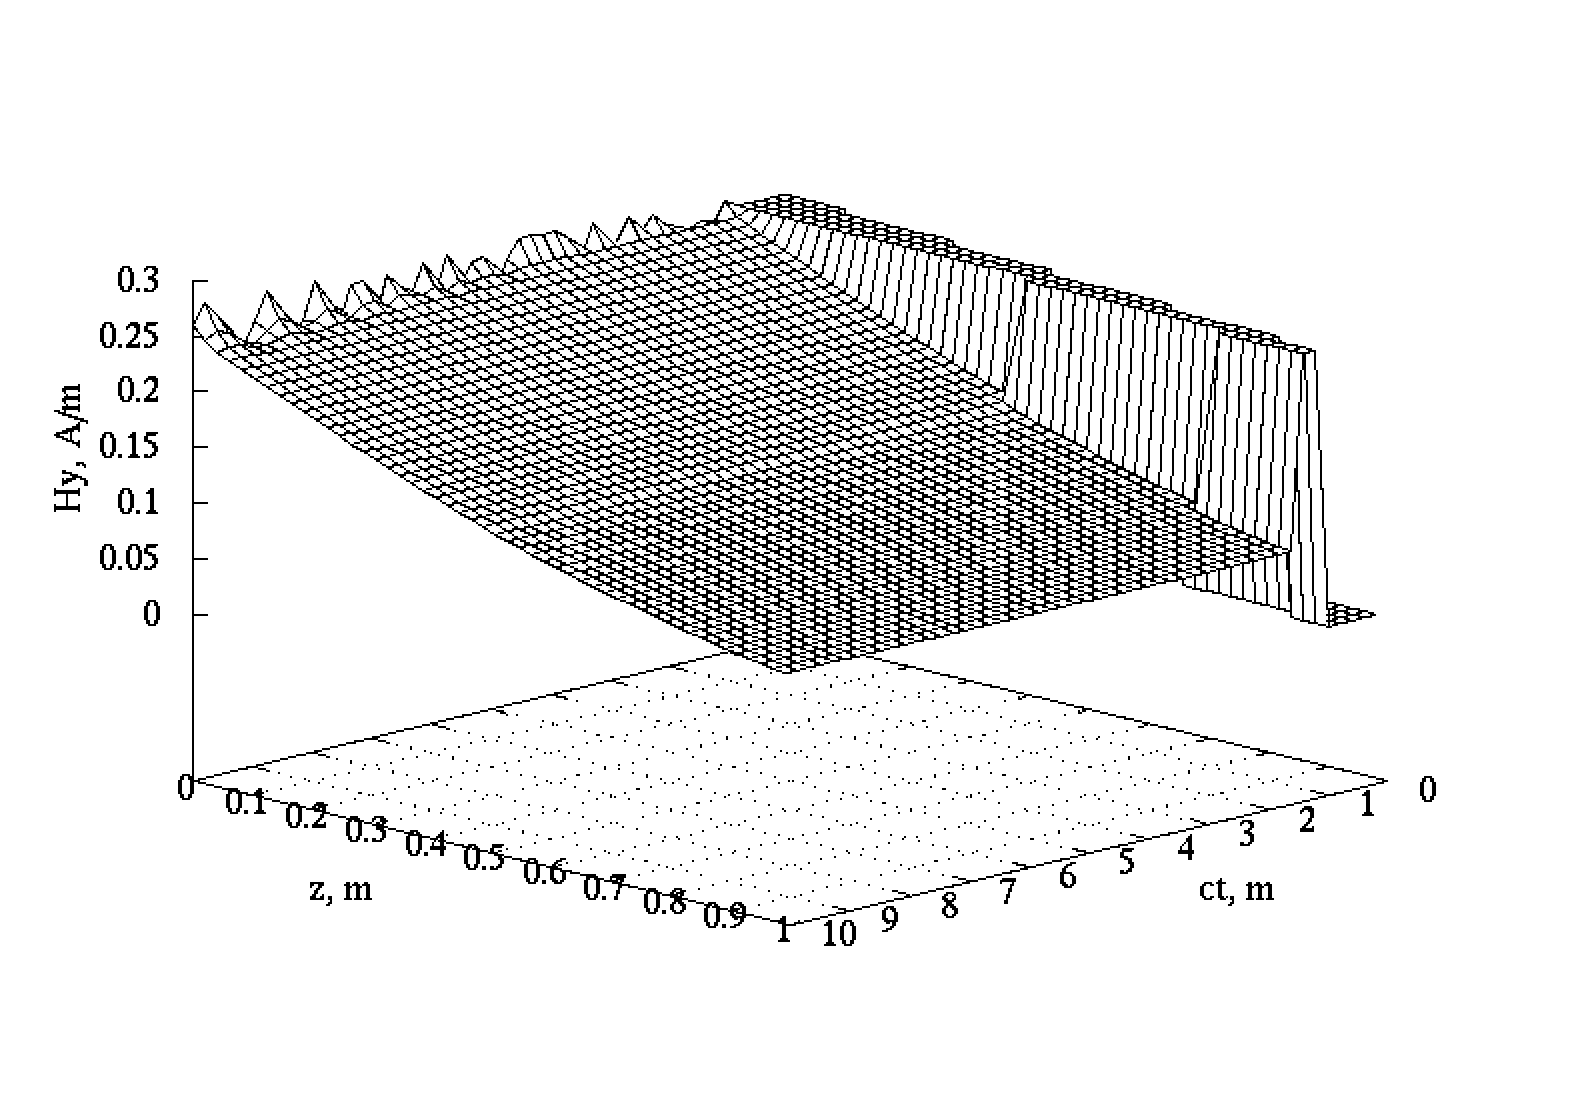
\includegraphics[scale=0.6]{StaticOnAxis}
\caption{Магнітно-статичне поле ($ \rho = 0 $ м)} \label{fig:emp_h_rho}
\end{center} \end{figure}
%
\begin{figure}[h] \begin{center}
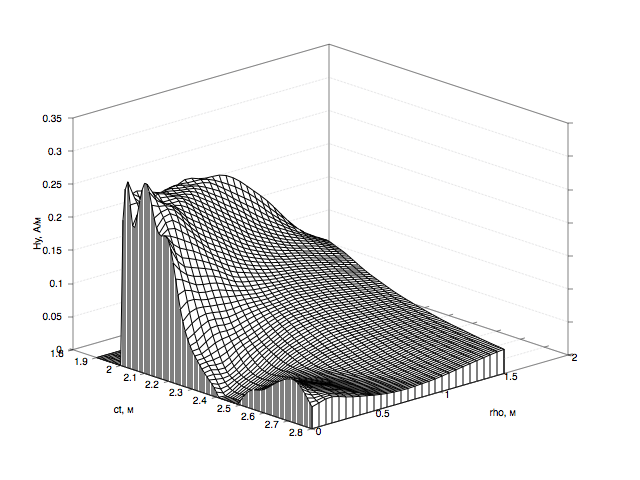
\includegraphics[scale=0.7]{LinearMagnetic}
\caption{Магнітно-статичне поле ($ z = 2 $ м)} \label{fig:emp_h_rho}
\end{center} \end{figure}

За визначенням дальньої зони - це область простору, де $ E_\varphi = H_\rho $ та
$ H_\varphi = E_\rho $. Дня лінійного поля плаского диску ці умови виконується, 
коли $ U_0(W_-,Z) - U_2(W_-,Z) = J_0(Z) $. Остання тотожність математично вірна
тоді і тільки коли 
%
\begin{equation} \label{eq:FraunhoferDistance}
\left. \lim_{z \to \infty} \left( \frac{ct-z}{ct+z} \right)^m 
\right|_{m > 1} = 0
\end{equation}

Остання тотожність є умовою дальньої зони для антени що породжує 
нестаціонарне поле. Варто зазначити, що при рості $ z $ росте і $ t $, 
відповідно до принципу причинності, тобто умова $ ct - z > 0 $ виконується.

%%%%%%%%%%%%%%%%%%%%%%%%%%%%%%%%%%%%%%%%%%%%%%%%%%%%%%%%%%%%%%%%%%%%%%%%%%%%%%%%
\section{Вторинне джерело поля в слабкому нелінійному середовищі. 
Нелінійність Керра}

При взаємодії з середовищем поле змінюється. Така повединка називається ефектом 
самодії. Джерелом такого поля стає весь простір його розповсюдження. Назвемо 
таке джерело вторинним. Випадки коли вторинним джерелом можна знехтувати, за 
рахунок його незначного вливу порівняно з первинним джерелом, називається 
лінійною задачею випромінювання. Прикладами такого поля є 
\eqref{eq:linear_h_cyl} та \eqref{eq:linear_e_cyl}. Тепер розглянемо 
середовище, де вплив самодії все ще незначний порівнянно з лінійним полем, але
викликає розбіжності в емпіричних показниках та данних теоретичної моделі. 
Таке середовище називають слабним нелінійним середовищем. Вторинне джерело 
поля в такому середовищі є функцією амплатуди поля. В якості такого джерела 
розглянемо вторинній електричний струм
%
\begin{equation*} 
\vect{J^\prime} = \partder{}{t} \vect{P^\prime} \left( \vect{E} \right)
\end{equation*}

Остання рівність складається з двох додаків. Перший додаток відповідає саме 
нелінійним властивостям поля. Останній додаток описує провідникові властивості 
середи розповлюдження, які теж мжуть бути описані вторинним джерелом. 
%
\begin{equation*} 
\vect{J^\prime} = 
\vect{\rho_0}    \partder{}{t} P_\rho^\prime    \left( \vect{E} \right) + 
\vect{\varphi_0} \partder{}{t} P_\varphi^\prime \left( \vect{E} \right) + 
\vect{z_0}       \partder{}{t} P_z^\prime       \left( \vect{E} \right) 
\end{equation*}
%
Вектор поляризвції для середовищі, де спостерігаюсься слабкі нелінійні ефкекти 
є довільною функцією, але може бути представлено в виді розкладу степеневого 
ряду Тейлора. 
%
\begin{equation*} \begin{aligned}
\vect{P^\prime} \left( \vect{E} \right) = \sum_{i=2}^{\infty} \xi_i \vect{E}^i
\end{aligned} \end{equation*}
%
Зауважимо, що розклад ведется по степеням вектора напружиності 
електричного поля, як у задачах оптики \textcolor{red}{[ПОСИЛАННЯ]}. 
Це створює математичні проблеми у доданках з парними коефіцієнтами.
вирішити їх можна домноженням на одиничний вектор.
%
\begin{equation*} \begin{aligned}
\vect{P^\prime}_2 \left( \vect{E} \right) = \xi_2 \vect{E}^2 = 
\xi_2 \vect{E}^2 \left( \vect{\rho_0}  + \vect{\varphi_0} + \vect{z_0} \right)
\end{aligned} \end{equation*}
%
\textcolor{red}{ Згідно з неоднозначностю векторного потенціалу 
\cite[ст. 77]{imp:LandauII} $ \vect{J^\prime} \left\{ S_1 \right\}  = 0 $. }
%
\textcolor{red}{ Чи правильно, що нелінійна ппроникність поля залежеть від 
амплтуди джерела? }
%
Для аналізу виберемо третій доданок неліної поляризації, який активно 
використовується в імпульсній електроніці \textcolor{red}{[ПОСИЛАННЯ]}.
%
\begin{equation*}
\vect{P^\prime} \left( \vect{E} \right) = 
\xi_3^e \vect{E}^3 
\left( A_0, R, \epsilon, \mu, vt, \vect{r} \right)
\end{equation*}
%
Під кубом вектора розуміється сам вектор домноженій на квадрат довжини.
\textcolor{red}{ Можливо, що природа нелінійних ефектів значно глибша і 
їх ефект впливає на характер енегетичної взаємодії та змінює простір.
Відповідно довжина вектора в декартовому сенсі втрачає змаст. }
%
\begin{equation*}
\vect{P^\prime} \left( \vect{E} \right) = 
\xi_3^e \dotprod{ \vect{E} }{ \vect{E} } \cdot \vect{E} 
\end{equation*}
%
В середовищі, де нелінійні ефекти описуються таким вектором
%
\textcolor{lightgray}{ \begin{equation*} \begin{aligned}
\vect{P^\prime} \left( \vect{E} \right) = 
\frac{ {A_0}^3 \xi_3^e }{ 8 } \left( \frac{\mu_0 \mu}
{\epsilon_0 \epsilon} \right)^{3/2} \left( {I_1}^2 \cos^2 \varphi + 
\left( I_2 - I_1 \right)^2 \sin^2 \varphi \right) \cdot \\ 
\cdot \Big( \vect{\rho_0} I_1 \cos \varphi - 
\vect{ \varphi_0 } \left( I_2 - I_1 \right) \sin \varphi \Big)
\end{aligned} \end{equation*} }
%
\textcolor{red}{ Які нелінійні ефекти спостерігаються в керрівському середовищі?}

%%%%%%%%%%%%%%%%%%%%%%%%%%%%%%%%%%%%%%%%%%%%%%%%%%%%%%%%%%%%%%%%%%%%%%%%%%%%%%%%
\section{Еволюційні коефіцієнти для нелінійної поправки до поля}
%
Для отримання нелінійної поправки до електричного поля спочатку отримаємо
розкладене по модовому базису вторинне джерело поля. Для цього, 
\textcolor{red}{згідно принципам віпромінювання}, знадобляться 
похідні компонентів електричного поля за часом. Часова залежність лінійного
електричного поля плаского дику міститься тільки в функціях 
$ I_1(ct,r) $ та $ I_2(ct,r) $. Для збереження безрозмарності розділимо
похідні на максимальну швидкість розповсюдженя для середовища.
%
\textcolor{lightgray}{ \begin{equation*} \begin{aligned}
I_1 \left\{ S_2 \right\} = \frac{\rho^2 + R^2}{4 \pi \rho^2} \arccos 
\frac{c^2 t^2 - z^2 - \rho^2 - R^2}{2 \rho R}  -
\frac{\sqrt{4 \rho^2 R^2 - (\rho^2 + R^2 - c^2t^2 + z^2)^2}}{4 \pi \rho^2} - \\
- \frac{ |\rho^2 - R^2| }{2 \pi \rho^2} 
\arctan \sqrt{ \frac{(\rho - R)^2}{(\rho + R)^2} \cdot
\frac{\left( \rho + R \right)^2 - \left( c^2t^2 - z^2 \right)} 
{\left( c^2t^2 - z^2 \right) - \left( \rho - R \right)^2} }
\end{aligned} \end{equation*} }
%
\textcolor{lightgray}{ \begin{equation*} \begin{aligned}
\partder{I_1 \left\{ S_2 \right\}}{t} = \frac{\rho^2 + R^2}{4 \pi \rho^2}
\partder{}{t} \arccos \frac{c^2 t^2 - z^2 - \rho^2 - R^2}{2 \rho R} - \\
- \partder{}{t} \frac{\sqrt{4 \rho^2 R^2 - (\rho^2 + R^2 - c^2t^2 + z^2)^2}}
{4 \pi \rho^2} - \\ - \frac{ |\rho^2 - R^2| }{2 \pi \rho^2} \partder{}{t} 
\arctan \sqrt{ \frac{(\rho - R)^2}{(\rho + R)^2} \cdot
\frac{\left( \rho + R \right)^2 - \left( c^2t^2 - z^2 \right)} 
{\left( c^2t^2 - z^2 \right) - \left( \rho - R \right)^2} }
\end{aligned} \end{equation*} }
%
\textcolor{lightgray}{ \begin{equation*} \begin{aligned}
\partder{}{t} \arccos \frac{c^2 t^2 - z^2 - \rho^2 - R^2}{2 \rho R} = 
- \frac{2 c^2 t}
{ \sqrt{4 \rho^2 R^2 - \left(c^2 t^2 - z^2 - \rho^2 - R^2 \right)^2} }
\end{aligned} \end{equation*} }
%
\textcolor{red}{ \begin{equation*} \begin{aligned}
- \partder{}{t} \left( \rho^2 + R^2 - c^2t^2 + z^2 \right)^2 = 
- 2 (\rho^2 + R^2 -c^2t^2 + z^2) (-2 c^2 t)
\end{aligned} \end{equation*} }
%
\textcolor{lightgray}{ \begin{equation*} \begin{aligned}
\partder{}{t} \frac{\sqrt{4 \rho^2 R^2 - (\rho^2 + R^2 - c^2t^2 + z^2)^2}}
{4 \pi \rho^2} = \frac{1}{8 \pi \rho^2} 
\frac{ 4 c^2 t (\rho^2 + R^2 - c^2 t^2 + z^2) }
{ \sqrt{4 \rho^2 R^2 - (\rho^2 + R^2 - c^2t^2 + z^2)^2} } = \\
= \frac{c^2 t}{2 \pi \rho^2} \frac{\rho^2 + R^2 - c^2 t^2 + z^2}
{ \sqrt{4 \rho^2 R^2 - (\rho^2 + R^2 - c^2t^2 + z^2)^2} }
\end{aligned} \end{equation*} }
%
\textcolor{red}{ \begin{equation*} \begin{aligned}
\partder{}{t} \arctan \sqrt{ \frac{x}{y} } = 
\frac{1}{1 + \frac{x}{y}} \frac{1}{2} 
\sqrt \frac{y}{x} \partder{}{t} \frac{x}{y}
\end{aligned} \end{equation*} }
%
\textcolor{red}{ \begin{equation*} \begin{aligned}
- \frac{1}{(\rho + R)^2} + \frac{1}{(\rho - R)^2} = 
\frac{- (\rho-R)^2 + (\rho+R)^2 }{ (\rho^2 - R^2)^2 }
\end{aligned} \end{equation*} }
%
\textcolor{lightgray}{ \begin{equation*} \begin{aligned}
\partder{}{t} \arctan \sqrt{ \frac{(\rho - R)^2}{(\rho + R)^2}
\frac{\left( \rho + R \right)^2 - \left( c^2t^2 - z^2 \right)} 
{\left( c^2t^2 - z^2 \right) - \left( \rho - R \right)^2} } = 
\partder{}{t} \arctan \sqrt{ \frac
{1 - \frac{c^2t^2 - z^2}{\left( \rho + R \right)^2} } 
{ \frac{c^2t^2 - z^2}{ \left( \rho - R \right)^2 } - 1} } = \\
= \frac{1}{1 + \frac{1 - \frac{c^2t^2 - z^2}{\left( \rho + R \right)^2} } 
{ \frac{c^2t^2 - z^2}{ \left( \rho - R \right)^2 } - 1} } \frac{1}{2}
\sqrt{ \frac{ \frac{c^2t^2 - z^2}{ \left( \rho - R \right)^2 } - 1 }
{1 - \frac{c^2t^2 - z^2}{\left( \rho + R \right)^2} } } 
\frac{ - \frac{2 c^2 t}{\left( \rho + R \right)^2} 
\left( \frac{c^2t^2 - z^2}{ \left( \rho - R \right)^2} - 1 \right) - 
\frac{ 2 c^2 t }{ \left( \rho - R \right)^2 } 
\left( 1 - \frac{c^2t^2 - z^2}{\left( \rho + R \right)^2} \right) }
{\left( \frac{c^2t^2 - z^2}{ \left( \rho - R \right)^2 } - 1 \right)^2} = \\
= - c^2 t \frac{ \frac{c^2t^2-z^2}{(\rho-R)^2} - 1 }
{ \frac{c^2t^2-z^2}{(\rho-R)^2} - 1 + 1 - 
\frac{c^2t^2 - z^2}{\left( \rho + R \right)^2} }
\sqrt{ \frac{ \frac{c^2t^2 - z^2}{ \left( \rho - R \right)^2 } - 1}
{1 - \frac{c^2t^2 - z^2}{\left( \rho + R \right)^2} } } \frac
{ \frac{c^2t^2 - z^2}{ \left( \rho^2 - R^2 \right)^2 } - \frac{1}{(\rho+R)^2} + 
\frac{1}{(\rho-R)^2} - \frac{ c^2t^2 - z^2 }{ \left( \rho^2 - R^2 \right)^2 } }
{ \left( \frac{c^2t^2 - z^2}{ \left( \rho - R \right)^2} - 1 \right)^2 } = \\
= - \frac{4 \rho R c^2 t}{ \left( \rho^2 - R^2 \right)^2 } 
\frac{ 1 }{ \frac{c^2t^2-z^2}{(\rho-R)^2} - 
\frac{c^2t^2 - z^2}{\left( \rho + R \right)^2} }
\sqrt{ \frac{ \frac{c^2t^2 - z^2}{ \left( \rho - R \right)^2 } - 1}
{1 - \frac{c^2t^2 - z^2}{\left( \rho + R \right)^2} } } \frac
{ 1 }{ \frac{c^2t^2 - z^2}{ \left( \rho - R \right)^2} - 1 } = \\
= - \frac{c^2 t}{ c^2 t^2 - z^2 } \frac{1} { 
\sqrt{ 1 - \frac{c^2t^2 - z^2}{(\rho + R)^2 } } 
\sqrt{ \frac{c^2t^2 - z^2}{ (\rho - R)^2 } - 1} }
\end{aligned} \end{equation*} }
%
\textcolor{lightgray}{ \begin{equation*} \begin{aligned}
\partder{ I_1 \{ S_2 \} }{t} = - \frac{c^2 t}{2 \pi \rho^2}
\frac{\rho^2 + R^2}
{ \sqrt{4 \rho^2 R^2 - \left(c^2 t^2 - z^2 - \rho^2 - R^2 \right)^2} } - \\
- \frac{c^2 t}{2 \pi \rho^2} \frac{\rho^2 + R^2 - c^2 t^2 + z^2}
{ \sqrt{4 \rho^2 R^2 - (\rho^2 + R^2 - c^2t^2 + z^2)^2} } + \\ 
+ \frac{ c^2 t }{2 \pi \rho^2} \frac{|\rho^2 - R^2|}{ c^2 t^2 - z^2 } \frac{1} 
{ \sqrt{ 1 - \frac{c^2t^2 - z^2}{(\rho + R)^2 } } 
\sqrt{ \frac{c^2t^2 - z^2}{ (\rho - R)^2 } - 1} }
\end{aligned} \end{equation*} }
%
\begin{equation*} \begin{aligned}
\frac{1}{c} \partder{ I_1 \{ S_2 \} }{t} = \frac{ ct }{2 \pi \rho^2} 
\frac{ (\rho^2 - R^2)^2  (c^2 t^2 - z^2)^{-1} } 
{ \sqrt{ (\rho + R)^2 - c^2t^2 + z^2 } 
\sqrt{ c^2t^2 - z^2 - (\rho - R)^2 } } - \\
- \frac{ct}{2 \pi \rho^2} \frac{2 (\rho^2 + R^2) - (c^2 t^2 - z^2)}
{ \sqrt{4 \rho^2 R^2 - (c^2t^2 - z^2 - \rho^2 - R^2)^2} }
\end{aligned} \end{equation*}
%
\begin{equation*} \begin{aligned}
\frac{1}{c} \partder{ I_1 \{ S_{1,3} \} }{t} = 0
\end{aligned} \end{equation*}
%
\textcolor{lightgray}{ \begin{equation*} \begin{aligned}
\partder{ I_2 \{ S_2 \} }{t} = \frac{1}{\pi} \partder{}{t} \arccos 
\frac{c^2t^2 - z^2 + \rho^2 - R^2}{2 \rho \sqrt{c^2t^2 - z^2}} = \\
= - \frac{1}{\pi} \frac{1} { \sqrt{ 1 - \frac{ (c^2t^2 - z^2 + \rho^2 - R^2)^2 }
{4 \rho^2 (c^2t^2 - z^2)^2} } } \frac{1}{2 \rho} \partder{}{t} 
\frac{c^2t^2 - z^2 + \rho^2 - R^2} {\sqrt{c^2t^2 - z^2}} = \\
= - \frac{1}{2 \rho \pi} \frac{1} 
{ \sqrt{ 1 - \frac{ (c^2t^2 - z^2 + \rho^2 - R^2)^2 }
{4 \rho^2 (c^2t^2 - z^2)} } } \frac{2c^2t \sqrt{c^2t^2 - z^2} - 
\frac{c^2t}{\sqrt{c^2t^2 - z^2}} (c^2t^2 - z^2 + \rho^2 - R^2)
}{c^2t^2 - z^2} = \\ = - \frac{c^2 t}{2 \pi \rho} \frac{1} 
{ \sqrt{ 1 - \frac{ (c^2t^2 - z^2 + \rho^2 - R^2)^2 }
{4 \rho^2 (c^2t^2 - z^2)} } } \frac{2 \sqrt{c^2t^2 - z^2} - 
\frac{c^2t^2 - z^2 + \rho^2 - R^2}{\sqrt{c^2t^2 - z^2}}}{c^2t^2 - z^2} = \\
= - \frac{c^2 t}{2 \pi \rho (c^2t^2 - z^2)} \frac{ 2 \sqrt{c^2t^2 - z^2} - 
\frac{c^2t^2 - z^2 + \rho^2 - R^2}{\sqrt{c^2t^2 - z^2}} } 
{ \sqrt{ 1 - \frac{ (c^2t^2 - z^2 + \rho^2 - R^2)^2 }
{4 \rho^2 (c^2t^2 - z^2)} } } = \\
= - \frac{c^2 t}{\pi (c^2t^2 - z^2) } 
\frac{ 2 (c^2t^2 - z^2) - (c^2t^2 - z^2 + \rho^2 - R^2) } 
{ \sqrt{ 4 \rho^2 (c^2t^2 - z^2) - (c^2t^2 - z^2 + \rho^2 - R^2)^2 } } = \\
= - \frac{c^2 t}{\pi (c^2t^2 - z^2) } \frac{ c^2t^2 - z^2 -  \rho^2 + R^2 } 
{ \sqrt{ 4 \rho^2 (c^2t^2 - z^2) - (c^2t^2 - z^2 + \rho^2 - R^2)^2 } }
\end{aligned} \end{equation*} }
%
\begin{equation*} \begin{aligned}
\frac{1}{c} \partder{ I_2 \{ S_2 \} }{t} = 
- \frac{ct}{\pi (c^2t^2 - z^2) } \frac{ c^2t^2 - z^2 -  \rho^2 + R^2 } 
{ \sqrt{ 4 \rho^2 (c^2t^2 - z^2) - (c^2t^2 - z^2 + \rho^2 - R^2)^2 } }
\end{aligned} \end{equation*}
%
\begin{equation*} \begin{aligned}
\frac{1}{c} \partder{ I_2 \{ S_{1,3} \} }{t} = 0
\end{aligned} \end{equation*}
%
Тепер запишемо компоненти електричного струму, який є вторинним джерелом
електромагнітного поля. З компонентою $ \vect{z_0} $ все просто - 
поздовжне електричне поле дорівнює нулю.
%
\textcolor{lightgray}{ \begin{equation*} \begin{aligned}
\vect{P^\prime} \left( \vect{E} \right) = 
\frac{ {A_0}^3 \xi_3 }{ 8 } \left( \frac{\mu_0 \mu}
{\epsilon_0 \epsilon} \right)^{3/2} \left( {I_1}^2 \cos^2 \varphi + 
\left( I_2 - I_1 \right)^2 \sin^2 \varphi \right) \cdot \\ 
\cdot \Big( \vect{\rho_0} I_1 \cos \varphi - 
\vect{ \varphi_0 } \left( I_2 - I_1 \right) \sin \varphi \Big)
\end{aligned} \end{equation*} }
%
\textcolor{lightgray}{ \begin{equation*} \label{eq:linear_e_cyl}
\vect{E} = \frac{A_0}{2} \sqrt{\frac{\mu_0 \mu}{\epsilon_0 \epsilon}}
\Big( \vect{\rho_0} I_1 \cos \varphi - 
\vect{ \varphi_0 } \left( I_2 - I_1 \right) \sin \varphi \Big)
\end{equation*} }
%
\textcolor{lightgray}{ \begin{equation*} \begin{aligned}
\vect{E}^2 = \frac{A_0^2}{4} \frac{\mu_0 \mu}{\epsilon_0 \epsilon}
\Big( I_1^2 \cos^2 \varphi + \left( I_2 - I_1 \right)^2 \sin^2 \varphi \Big)
\end{aligned} \end{equation*} }
%
\textcolor{lightgray}{ \begin{equation*} \begin{aligned}
\partder{ \vect{E}^2 }{t} = \frac{A_0^2}{4} 
\frac{\mu_0 \mu}{\epsilon_0 \epsilon}
\left( 2 I_1 \partder{I_1}{t} \cos^2 \varphi + 
2 ( I_2 - I_1 ) \left( \partder{I_2}{t} - \partder{I_1}{t} \right) 
\sin^2 \varphi \right)
\end{aligned} \end{equation*} }
%
\begin{equation*} \begin{aligned}
\partder{P_z^\prim}{t} = 0
\end{aligned} \end{equation*}
%
Вирази для поперечних компонентів поля стають шматочновизначиними,
через свої залежності.
%
\textcolor{lightgray} { \begin{equation*} \begin{aligned}
\partder{P_\rho^\prime}{t}   = \frac{ {A_0}^3 \xi_3 }{ 8 } 
\left( \frac{\mu_0 \mu} {\epsilon_0 \epsilon} \right)^{3/2} \left(
\left( {I_1}^2 \cos^2 \varphi + ( I_2 - I_1 )^2 \sin^2 \varphi \right)
\partder{I_1}{t} \cos \varphi + \right. \\
\left. + I_1 \cos \varphi \left( 2 I_1 \partder{I_1}{t} \cos^2 \varphi + 
2 ( I_2 - I_1 ) \left( \partder{I_2}{t} - \partder{I_1}{t} \right) 
\sin^2 \varphi \right) \right) = \\ = \frac{ {A_0}^3 \xi_3^e }{ 8 } 
\left( \frac{\mu_0 \mu} {\epsilon_0 \epsilon} \right)^{3/2} \left(
\partder{I_1}{t} {I_1}^2 \cos^3 \varphi + \partder{I_1}{t} ( I_2 - I_1 )^2 
\cos \varphi \sin^2 \varphi + \right. \\
\left. + 2 {I_1}^2 \partder{I_1}{t} \cos^3 \varphi + 
2 I_1 ( I_2 - I_1 ) \left( \partder{I_2}{t} - \partder{I_1}{t} \right) 
\cos \varphi \sin^2 \varphi \right)
\end{aligned} \end{equation*} }
%
\begin{equation*} \begin{aligned}
\partder{P_\rho^\prime}{t} = \frac{ {A_0}^3 \xi_3 }{ 8 } 
\left( \frac{\mu_0 \mu} {\epsilon_0 \epsilon} \right)^{3/2} \left(
3 {I_1}^2 \partder{I_1}{t} \cos^3 \varphi + \right. \\
+ \left. ( I_2 - I_1 ) \cos \varphi \sin^2 \varphi \left( 
\partder{I_1}{t} ( I_2 - I_1 ) + 2 I_1 \left( \partder{I_2}{t} - 
\partder{I_1}{t} \right) \right) \right)
\end{aligned} \end{equation*}
%
\textcolor{lightgray} { \begin{equation*} \begin{aligned}
\partder{P_\varphi^\prime}{t}   = - \frac{ {A_0}^3 \xi_3 }{ 8 } 
\left( \frac{\mu_0 \mu} {\epsilon_0 \epsilon} \right)^{3/2} \left(
\left( {I_1}^2 \cos^2 \varphi + ( I_2 - I_1 )^2 \sin^2 \varphi \right)
\left( \partder{I_2}{t} - \partder{I_1}{t} \right) \sin \varphi + \right. \\
\left. + (I_2 - I_1) \sin \varphi \left( 2 I_1 \partder{I_1}{t} \cos^2 \varphi + 
2 ( I_2 - I_1 ) \left( \partder{I_2}{t} - \partder{I_1}{t} \right) 
\sin^2 \varphi \right) \right) = \\ = - \frac{ {A_0}^3 \xi_3 }{ 8 } 
\left( \frac{\mu_0 \mu} {\epsilon_0 \epsilon} \right)^{3/2} \left(
{I_1}^2 \left( \partder{I_2}{t} - \partder{I_1}{t} \right) 
\sin \varphi \cos^2 \varphi + \right. \\ \left. 
+ ( I_2 - I_1 )^2 \left( \partder{I_2}{t} - \partder{I_1}{t} \right) 
\sin^3 \varphi + 2 I_1 \partder{I_1}{t} (I_2 - I_1) 
\sin \varphi \cos^2 \varphi + \right. \\ 
+ \left. 2 ( I_2 - I_1 )^2 \left( \partder{I_2}{t} - \partder{I_1}{t} \right) 
\sin^3 \varphi \right)
\end{aligned} \end{equation*} }
%
\begin{equation*} \begin{aligned}
\partder{P_\varphi^\prime}{t} = - \frac{ {A_0}^3 \xi_3 }{ 8 } 
\left( \frac{\mu_0 \mu} {\epsilon_0 \epsilon} \right)^{3/2} \left(
3 ( I_2 - I_1 )^2 \left( \partder{I_2}{t} - \partder{I_1}{t} \right)
\sin^3 \varphi \right. + \\
+ \left. I_1 \sin \varphi \cos^2 \varphi \left( 
I_1 \left( \partder{I_2}{t} - \partder{I_1}{t} \right) + 
2 \partder{I_1}{t} (I_2 - I_1) \right) \right)
\end{aligned} \end{equation*}
%
Для запису модового струму використаємо формулу ..., що 
є кратиним інтегралом по точкам випромінювання та має комплексну
область значень.
%
\textcolor{lightgray} { \begin{equation*}
j_m \left( r, t; \nu \right) = \frac{\sqrt{\mu_0}}{2\pi} 
\int \limits_{0}^{2\pi} d \varphi \int \limits_0^\infty \rho d \rho 
\vect{j_0} \crossprod{ \nabla_\perp \Psi_m^* }{ \vect{z_0} }
\end{equation*} }
%
\textcolor{lightgray} { \begin{equation*} 
\vect{J^\prime} = 
\vect{\rho_0}    \partder{}{t} P_\rho^\prime    \left( \vect{E} \right) + 
\vect{\varphi_0} \partder{}{t} P_\varphi^\prime \left( \vect{E} \right) + 
\vect{z_0}       \partder{}{t} P_z^\prime       \left( \vect{E} \right) 
\end{equation*} }
%
\textcolor{lightgray} { \begin{equation*} \begin{aligned}
\crossprod{ \nabla_\perp \Psi_m^* }{ \vect{z_0} } =
- \vect{\rho_0} i m e^{-im\varphi} \frac{J_m (\nu \rho)}{\rho \sqrt{\nu}}
- \vect{\varphi_0} \sqrt{\nu} e^{-im\varphi} 
\frac{J_{m-1} (\nu \rho) - J_{m+1} (\nu \rho)}{2}
\end{aligned} \end{equation*} }
%
\textcolor{lightgray} { \begin{equation*} \begin{aligned}
\vect{J^\prime} \crossprod{ \nabla_\perp \Psi_m^* }{ \vect{z_0} } = 
- i e^{-im\varphi} m \frac{J_m (\nu \rho)}{\rho \sqrt{\nu}}
\partder{}{t} P_\rho^\prime \left( \vect{E} \right) - \\
- \sqrt{\nu} e^{-im\varphi} \frac{J_{m-1} (\nu \rho) - J_{m+1} (\nu \rho)}{2}
\partder{}{t} P_\varphi^\prime \right)
\end{aligned} \end{equation*} }
%
\begin{equation*} \begin{aligned}
j_m = - \frac{\sqrt{\mu_0}}{2\pi} 
\int_{0}^{2\pi} d \varphi \int \limits_{0}^{\infty} \rho d \rho
e^{-im\varphi} \left( i  m \frac{J_m (\nu \rho)}{\rho \sqrt{\nu}}
\partder{P_\rho^\prime}{t} + \sqrt{\nu}
\frac{J_{m-1} (\nu \rho) - J_{m+1} (\nu \rho)}{2}
\partder{P_\varphi^\prime}{t} \right)
\end{aligned} \end{equation*}
%
Згрупувавши доданки за тригонометричними функціями, що вони містять,
знайдемо інтеграли за зменним азимутальним кутом $ \varphi $. Самі інеграли
взяті окремо в додатку ..., випишимо лише результати.
%
\textcolor{lightgray} { \begin{equation*} \begin{aligned}
\int_{0}^{2 \pi} d \varphi e^{-im \varphi} \partder{P_\rho^\prime}{t} = 
\frac{ {A_0}^3 \xi_3 }{ 8 } \int_{0}^{2\pi} d \varphi
e^{-im\varphi} \left( \frac{\mu_0 \mu} {\epsilon_0 \epsilon} \right)^{3/2} 
\left( 3 {I_1}^2 \partder{I_1}{t} \cos^3 \varphi + \right. \\
+ \left. ( I_2 - I_1 ) \cos \varphi \sin^2 \varphi \left( 
\partder{I_1}{t} ( I_2 - I_1 ) + 2 I_1 \left( \partder{I_2}{t} - 
\partder{I_1}{t} \right) \right) \right) = \\
= \frac{ {A_0}^3 \xi_3 }{ 8 } 
\left( \frac{\mu_0 \mu} {\epsilon_0 \epsilon} \right)^{3/2}
\left( \frac{3 \pi}{4} {I_1}^2 \partder{I_1}{t} \left( \delta_{m,-3} - 
\delta_{m,3} + 3 \delta_{m,-1} + 3 \delta_{m,1} \right) + \right. \\
+ \frac{\pi }{4} \left. ( I_2 - I_1 ) \left( \delta_{m,1} - 
\delta_{m,-3} + \delta_{m,-1} - \delta_{m,3} \right) \left( 
\partder{I_1}{t} ( I_2 - I_1 ) + 2 I_1 \left( \partder{I_2}{t} - 
\partder{I_1}{t} \right) \right) \right)
\end{aligned} \end{equation*} }
%
\textcolor{lightgray} { \begin{equation*} \begin{aligned}
\int_{0}^{2\pi} e^{-i m \varphi} \cos^3 \varphi d \varphi = 
\frac{\pi}{4} \delta_{m,-3} - \frac{\pi}{4} \delta_{m,3} + 
\frac{3 \pi}{4} \delta_{m,-1} + \frac{3 \pi}{4} \delta_{m,1}
\end{aligned} \end{equation*} }
%
\textcolor{lightgray} { \begin{equation*} \begin{aligned}
\int_{0}^{2\pi} e^{-i m \varphi} \cos \varphi \sin^2 \varphi d \varphi = 
\frac{\pi \delta_{m,1} }{4} - \frac{\pi \delta_{m,-3} }{4} + 
\frac{\pi \delta_{m,-1} }{4} - \frac{\pi \delta_{m,3} }{4}
\end{aligned} \end{equation*} }
%
\begin{equation*} \begin{aligned}
\int_{0}^{2\pi} d \varphi e^{-im \varphi} \partder{P_\rho^\prime}{t} = 
\frac{ {A_0}^3 \xi_3 \pi }{ 4 \cdot 8 } 
\left( \frac{\mu_0 \mu} {\epsilon_0 \epsilon} \right)^{3/2}
\left( 3 {I_1}^2 \partder{I_1}{t} \left( \delta_{m,-3} - 
\delta_{m,3} + 3 \delta_{m,-1} + 3 \delta_{m,1} \right) + \right. \\
+ \left. ( I_2 - I_1 ) \left( \delta_{m,1} - 
\delta_{m,-3} + \delta_{m,-1} - \delta_{m,3} \right) \left( 
\partder{I_1}{t} ( I_2 - I_1 ) + 2 I_1 \left( \partder{I_2}{t} - 
\partder{I_1}{t} \right) \right) \right)
\end{aligned} \end{equation*}
%
\textcolor{lightgray} { \begin{equation*} \begin{aligned}
\int_{0}^{2\pi} e^{-i m \varphi} \sin^3 \varphi d \varphi = 
\frac{3 \pi i}{4} \delta_{m,-1} - \frac{3 \pi i}{4} \delta_{m,1} - 
\frac{\pi i}{4} \delta_{m,-3} - \frac{\pi i}{4} \delta_{m,3}
\end{aligned} \end{equation*} }
%
\textcolor{lightgray} { \begin{equation*} \begin{aligned}
\int_{0}^{2\pi} e^{-i m \varphi} \sin \varphi \cos^2 \varphi d \varphi = 
\frac{\pi i }{4} \delta_{m,-3} - \frac{\pi i }{4} \delta_{m,1} + 
\frac{\pi i }{4} \delta_{m,3} + \frac{\pi i }{4} \delta_{m,-1}
\end{aligned} \end{equation*} }
%
\textcolor{lightgray} { \begin{equation*} \begin{aligned}
\int_{0}^{2 \pi} d \varphi e^{-im \varphi} \partder{P_\varphi^\prime}{t} = \\
= - \frac{ {A_0}^3 \xi_3 }{ 8 } \int_{0}^{2 \pi} d \varphi e^{-im \varphi}
\left( \frac{\mu_0 \mu} {\epsilon_0 \epsilon} \right)^{3/2} \left(
3 ( I_2 - I_1 )^2 \left( \partder{I_2}{t} - \partder{I_1}{t} \right)
\sin^3 \varphi \right. + \\
+ \left. I_1 \sin \varphi \cos^2 \varphi \left( 
I_1 \left( \partder{I_2}{t} - \partder{I_1}{t} \right) + 
2 \partder{I_1}{t} (I_2 - I_1) \right) \right) = 
- \frac{ {A_0}^3 \xi_3 }{ 8 V } \cdot \\ 
\cdot \left( \frac{\mu_0 \mu} {\epsilon_0 \epsilon} \right)^{3/2} \left(
\frac{3 \pi i}{4} ( I_2 - I_1 )^2 \left( \partder{I_2}{t} - 
\partder{I_1}{t} \right) \left( 3 \delta_{m,-1} - 3 \delta_{m,1} - 
\delta_{m,-3} - \delta_{m,3} \right) \right. + \\
+ \left. \frac{\pi i}{4} I_1 \left(  \delta_{m,-3} - \delta_{m,1} + 
\delta_{m,3} + \delta_{m,-1} \right) \left( 
I_1 \left( \partder{I_2}{t} - \partder{I_1}{t} \right) + 
2 \partder{I_1}{t} (I_2 - I_1) \right) \right)
\end{aligned} \end{equation*} }
%
\begin{equation*} \begin{aligned}
\int_{0}^{2 \pi} d \varphi e^{-im \varphi} \partder{P_\varphi^\prime}{t} = 
- \frac{ {A_0}^3 \xi_3  i \pi }{ 4 \cdot 8 }
\left( \frac{\mu_0 \mu} {\epsilon_0 \epsilon} \right)^{3/2} \cdot \\ 
\cdot \left( 3 ( I_2 - I_1 )^2 \left( \partder{I_2}{t} - 
\partder{I_1}{t} \right) \left( 3 \delta_{m,-1} - 3 \delta_{m,1} - 
\delta_{m,-3} - \delta_{m,3} \right) \right. + \\
+ \left. I_1 \left(  \delta_{m,-3} - \delta_{m,1} + 
\delta_{m,3} + \delta_{m,-1} \right) \left( 
I_1 \left( \partder{I_2}{t} - \partder{I_1}{t} \right) + 
2 \partder{I_1}{t} (I_2 - I_1) \right) \right)
\end{aligned} \end{equation*}
%
\textcolor{lightgray} { \begin{equation*} \begin{aligned}
\int \limits_{0}^{2\pi} d \varphi \sin \varphi 
\left( \cos m \varphi - i \sin m \varphi \right) = 
i \pi \left( \delta_{m,-1} - \delta_{m,1} \right)
\end{aligned} \end{equation*} }
%
\textcolor{lightgray} { \begin{equation*} \begin{aligned}
\int \limits_{0}^{2\pi} d \varphi \cos \varphi 
( \cos m \varphi - i \sin m \varphi) = \pi ( \delta_{m,-1} + \delta_{m,1} )
\end{aligned} \end{equation*} }
%
Тепер введемо нові змінні для того, щоб записати струм в визначенні модового 
базису, як інтеграл за радиалькою координатою $ \rho $. Тут з'являються змінні
за штрихованими кординатами. Так ми означимо кординати джерела випромінювання,
щоб уникнути плутанини з кординатами точки спостереження. Нехай ...
%
\textcolor{lightgray} { \begin{equation*} \begin{aligned}
N_1 (m) =  \frac{3 m {A_0}^3 \xi_3 \sqrt{\mu_0}}{64 \sqrt{\nu}} \frac{\pi}{\pi}
\left( \frac{\mu_0 \mu} {\epsilon_0 \epsilon} \right)^{3/2} 
\int_{0}^{\infty} d \rho 
J_m (\nu \rho) {I_1}^2 \partder{I_1}{t}
\end{aligned} \end{equation*} }
%
\textcolor{lightgray} { \begin{equation*} \begin{aligned}
N_1 (m) =  3 m J_m (\nu \rho) {I_1}^2 \partder{I_1}{t}
\end{aligned} \end{equation*} }
%
\begin{equation*} \begin{aligned}
N_1 (m) =  3 m J_m (\nu \rho') {I_1}^2 \partder{I_1}{t'}
\end{aligned} \end{equation*}
%
\textcolor{lightgray} { \begin{equation*} \begin{aligned}
N_2 (m) = \frac{m {A_0}^3 \xi_3 \sqrt{\mu_0}}{64 \sqrt{\nu}} \frac{\pi}{\pi}
\left( \frac{\mu_0 \mu} {\epsilon_0 \epsilon} \right)^{3/2} 
\int_{0}^{\infty} d \rho \\
J_m (\nu \rho) (I_2 - I_1) \left( \partder{I_1}{t} (I_2 - I_1) + 
2 I_1 \left( \partder{I_2}{t} - \partder{I_1}{t} \right) \right)
\end{aligned} \end{equation*} }
%
\textcolor{lightgray} { \begin{equation*} \begin{aligned}
N_2 (m) = m J_m (\nu \rho) (I_2 - I_1) \left( \partder{I_1}{t} (I_2 - I_1) + 
2 I_1 \left( \partder{I_2}{t} - \partder{I_1}{t} \right) \right)
\end{aligned} \end{equation*} }
%
\begin{equation*} \begin{aligned}
N_2 (m) = m J_m (\nu \rho') (I_2 - I_1) \left( \partder{I_1}{t'} (I_2 - I_1) + 
2 I_1 \left( \partder{I_2}{t'} - \partder{I_1}{t'} \right) \right)
\end{aligned} \end{equation*}
%
\textcolor{lightgray} { \begin{equation*} \begin{aligned}
N_3 (m) = - \frac{3 {A_0}^3 \xi_3 \sqrt{\mu_0}}{64} \sqrt{\nu} \frac{\pi}{\pi}
\left( \frac{\mu_0 \mu} {\epsilon_0 \epsilon} \right)^{3/2} 
\int_{0}^{\infty} \rho d \rho 
\frac{J_{m-1} (\nu \rho) - J_{m+1} (\nu \rho)}{2} \\
(I_2 - I_1)^2 \left( \partder{I_2}{t} - \partder{I_1}{t} \right) 
\end{aligned} \end{equation*} }
%
\textcolor{lightgray} { \begin{equation*} \begin{aligned}
N_3 (m) = - 3 \nu \rho
\frac{J_{m-1} (\nu \rho) - J_{m+1} (\nu \rho)}{2}
(I_2 - I_1)^2 \left( \partder{I_2}{t} - \partder{I_1}{t} \right)
\end{aligned} \end{equation*} }
%
\begin{equation*} \begin{aligned}
N_3 (m) = - 3 \nu \rho'
\frac{J_{m-1} (\nu \rho') - J_{m+1} (\nu \rho')}{2}
(I_2 - I_1)^2 \left( \partder{I_2}{t'} - \partder{I_1}{t'} \right)
\end{aligned} \end{equation*}
%
\textcolor{lightgray} { \begin{equation*} \begin{aligned}
N_4 (m) = - \frac{ {A_0}^3 \xi_3 \sqrt{\mu_0}}{64} \sqrt{\nu} \frac{\pi}{\pi}
\left( \frac{\mu_0 \mu} {\epsilon_0 \epsilon} \right)^{3/2}
\int_{0}^{\infty} \rho d \rho 
\frac{J_{m-1} (\nu \rho) - J_{m+1} (\nu \rho)}{2} \\
I_1 \left( I_1 \left( \partder{I_2}{t} - \partder{I_1}{t} \right) + 
2 \partder{I_1}{t} \left( I_2 - I_1 \right) \right)
\end{aligned} \end{equation*} }
%
\textcolor{lightgray} { \begin{equation*} \begin{aligned}
N_4 (m) = - \nu \rho
\frac{J_{m-1} (\nu \rho) - J_{m+1} (\nu \rho)}{2}
\left( I_1 \left( \partder{I_2}{t} - \partder{I_1}{t} \right) + 
2 \partder{I_1}{t} \left( I_2 - I_1 \right) \right)
\end{aligned} \end{equation*} }
%
\begin{equation*} \begin{aligned}
N_4 (m) = - \nu \rho'
\frac{J_{m-1} (\nu \rho') - J_{m+1} (\nu \rho')}{2} I_1
\left( I_1 \left( \partder{I_2}{t'} - \partder{I_1}{t'} \right) + 
2 \partder{I_1}{t'} \left( I_2 - I_1 \right) \right)
\end{aligned} \end{equation*}
%
Тоді їх сумми для кожної з кутових мод матимуть наступний вигляд. 
%
\textcolor{lightgray} { \begin{equation*} \begin{aligned}
N_{-1}^{sum} =  i \delta_{m,-1} \left( 3 N_1 (m) + N_2 (m) + 
3 N_3 (m) + N_4 (m) \right)
\end{aligned} \end{equation*} }
%
\begin{equation*} \begin{aligned}
N_{-1}^{sum} = 3 N_1 (-1) + N_2 (-1) + 3 N_3 (-1) + N_4 (-1)
\end{aligned} \end{equation*}
%
\textcolor{lightgray} { \begin{equation*} \begin{aligned}
N_{1}^{sum} =  i \delta_{m,1} \left( 3 N_1 (m) + N_2 (m) - 
3 N_3 (m) - N_4 (m) ) \right)
\end{aligned} \end{equation*} }
%
\begin{equation*} \begin{aligned}
N_{1}^{sum} = 3 N_1 (1) + N_2 (1) - 3 N_3 (1) - N_4 (1)
\end{aligned} \end{equation*}
%
\textcolor{lightgray} { \begin{equation*} \begin{aligned}
N_{-3}^{sum} =  i \delta_{m,-3} \left( N_1 (m) - N_2 (m) - 
N_3 (m) + N_4 (m) \right)
\end{aligned} \end{equation*} }
%
\begin{equation*} \begin{aligned}
N_{-3}^{sum} = N_1 (-3) - N_2 (-3) - N_3 (-3) + N_4 (-3)
\end{aligned} \end{equation*}
%
\textcolor{lightgray} { \begin{equation*} \begin{aligned}
N_{3}^{sum} =  i \delta_{m,3} \left( - N_1 (m) - N_2 (m) - 
N_3 (m) + N_4 (m) \right)
\end{aligned} \end{equation*} }
%
\begin{equation*} \begin{aligned}
N_{3}^{sum} = - N_1 (3) - N_2 (3) - N_3 (3) + N_4 (3)
\end{aligned} \end{equation*}
%
Тепер запишимо модовий струм в нових зменних.
%
\begin{equation*} \begin{aligned}
j'_m (t',z') = - \frac{i \xi_3 A_0^3 \sqrt{\mu_0}}{64 \sqrt{\nu}}
\left( \frac{\mu_0 \mu} {\epsilon_0 \epsilon} \right)^{3/2}
\int_{0}^{\infty} N_{m}^{sum} (\rho',t',z') d \rho'
\end{aligned} \end{equation*}
%
Помічаємо деякі властивості нових змінних $ N_i(m) $
%
\textcolor{red} { \begin{equation*} \begin{aligned}
N_{-m} = N_{m}
\end{aligned} \end{equation*}  }
%
А також та $ N_i^{sum} $
%
\textcolor{red} { \begin{equation*} \begin{aligned}
N_{-m}^{sum} = N_{m}^{sum}
\end{aligned} \end{equation*}  }

%%%%%%%%%%%%%%%%%%%%%%%%%%%%%%%%%%%%%%%%%%%%%%%%%%%%%%%%%%%%%%%%%%%%%%%%%%%%%%%%
\section{Нелінійна поправка}
%
Тепер коли визначено джерело можна застосувати метод еволюційних рівнянь.
Почнемо з розв'язку рівняння Клейна-Гордона.
%
\begin{equation*}
\frac{\epsilon \mu}{ \sqrt{\epsilon_0 \mu_0}} 
\frac{\partial^2 h_m}{\partial t^2} - \frac{\partial^2 h_m}{\partial z^2} + 
\nu^2 h_m = j_m (t',z'; \nu)
\end{equation*}
%
Коефіцієнт $ h_m $ доведеться розраховувати чисельно за формолою
%
\begin{equation*}
h_m (z, t; \nu) = \int_{0}^{\infty} \int_{0}^{\infty}
j_m (t',z'; \nu) G(t,t',z,z') dz' dt'
\end{equation*}
%
де 
%
\begin{equation*}
G(t,t',z,z') = \frac{\mathit{V}}{2} H \left( \mathit{V} (t-t') - (z-z') \right)
J_0 \left( \nu \sqrt{\mathit{V}^2 (t-t')^2 - (z-z')^2} \right)
\end{equation*}
%
З $ h_m $ можна отримати інші магнітні коефіцієнти
%
\begin{equation*}
I_m^h = \partial_z (h_m)
\end{equation*}
%
\begin{equation*}
V_m^h = - \mu \partial_{ct} (h_m)
\end{equation*}
%
Аналогічно для продольного коєфіціенту електричного поля
%
\textcolor{lightgray}{ \begin{equation*}
- \partial_{ct}(\mu I_n^e) - \partial_z V_n^e + \chi^2 e_n = 0
\end{equation*} }
%
\textcolor{lightgray}{ \begin{equation*}
\epsilon \mu \partial_{ct} \left( \partial_{ct} e_n + 
\frac{\sqrt{\mu_0}}{2 \pi} \int_0^{2\pi} d \varphi 
\int_0^{\infty} \rho d \rho \Phi_n^* (\chi) J_z \right) - 
\partial^2_z e_n + \chi^2 e_n = 0
\end{equation*} }
%
\begin{equation*}
\frac{\epsilon \mu}{ \sqrt{\epsilon_0 \mu_0}} 
\frac{\partial^2 e_n}{\partial t^2} - 
\frac{\partial^2 e_n}{\partial z^2} + \chi^2 e_n = 
- \frac{\sqrt{\mu_0}}{2 \pi c} 
\int_0^{2\pi} d \varphi 
\int_0^{\infty} \rho d \rho \Phi_n^* (\chi) \partder{J_z}{t}
\end{equation*}
%
Поздовжний вторинний електричний струм рівний нулю, тому рівняння 
Клейна-Гордона для $ e_n (z, t; \chi) $ є однорідним та має нульовий розвязок.
%
\begin{equation*}
e_n (z, t; \chi) = \iint_S j_n (t',z', \chi) G(t,t',z,z') dt' dz' = 0
\end{equation*}
%
Також чисельно знайдемо розвязки еволюційних рівнянь, що залишились.
%
\textcolor{lightgray}{ \begin{equation*}
\partial_{ct} (\epsilon e_n) = - I_n^e - 
\frac{\sqrt{\mu_0}}{2 \pi} \int_0^{2\pi} d \varphi 
\int_0^{\infty} \rho d \rho \Phi_n^* (\chi) J_z
\end{equation*} }
%
\begin{equation*}
I_n^e = - \partial_{ct} (\epsilon e_n) - 
\frac{\sqrt{\mu_0}}{2 \pi} \int_0^{2\pi} d \varphi 
\int_0^{\infty} \rho d \rho \Phi_n^* (\chi) J_z
\end{equation*}
%
\begin{equation*}
\partial_{z} e_n = V_n^e
\end{equation*}
%
\textcolor{lightgray} { \begin{equation*} \begin{aligned}
\vect{E_\perp} = \frac{1}{\sqrt{\epsilon_0}} \left( 
\sum \limits_{m=-\infty}^{\infty} \int \limits_{0}^{\infty} 
d \nu V_m^h \crossprod{ \nabla_\perp \Psi_m }{ \vect{z_0} } +
\sum \limits_{n=-\infty}^{\infty} \int \limits_{0}^{\infty}
d \chi V_n^e \nabla_\perp \Phi_n \right)
\end{aligned} \end{equation*} }
%
\textcolor{lightgray} { \begin{equation*} \begin{aligned}
\crossprod{ \nabla_\perp \Psi_m }{ \vect{z_0} } = 
- e^{im\varphi} \left( \vect{\varphi_0} \sqrt{\nu} 
\frac{J_{m-1} (\nu \rho) - J_{m+1} (\nu \rho)}{2} - 
i m \vect{\rho_0} \frac{J_m (\nu \rho)}{ \rho \sqrt{\nu}} \right)
\end{aligned} \end{equation*} }
%
Останнам кроком для отримання результату мала стати чисельна оцінка 
інтегралів по безперервному модовому спектру $ \nu $. Для кожної з п'яти
компонентів поля.
%
\begin{equation*} \begin{aligned} \label{eq:KerrAmendErhoInit}
E_\rho = \frac{1}{\sqrt{\epsilon_0}} \sum_{m=-\infty}^{\infty} 
i m e^{im\varphi} \int_{0}^{\infty} \frac{d \nu}{\sqrt{\nu}} 
V_m^h \frac{J_m(\nu \rho)}{\rho}
\end{aligned} \end{equation*}
%
\begin{equation*} \begin{aligned}
E_\varphi = - \frac{1}{2 \sqrt{\epsilon_0}} \sum_{m=-\infty}^{\infty} 
e^{im\varphi} \int_{0}^{\infty} \sqrt{\nu} d \nu 
V_m^h \left( J_{m-1} (\nu \rho) - J_{m+1} (\nu \rho) \right)
\end{aligned} \end{equation*}
%
\begin{equation*} 
E_z = \frac{1}{\sqrt{\epsilon_0}} \sum_{n=-\infty}^{\infty}
\int_0^\infty \chi^2 d \chi e_n \Phi_n = 0
\end{equation*}
%
\textcolor{lightgray} { \begin{equation*}
\vect{H_\perp} = \frac{1}{\sqrt{\mu_0}} \left( 
\sum \limits_{m=-\infty}^{\infty} \int \limits_{0}^{\infty} d \nu
I_m^h \nabla_\perp \Psi_m + \sum \limits_{n=-\infty}^{\infty}
\int \limits_{0}^{\infty} d \chi I_n^e 
\crossprod{\vect{z_0}}{\nabla_\perp \Phi_n} \right)
\end{equation*} }
%
\textcolor{lightgray} { \begin{equation*} \begin{aligned}
\nabla_\perp \Psi_m = e^{i m \varphi} \left( \vect{\rho_0} 
\sqrt{\nu} \frac{ J_{m-1}(\nu \rho) - J_{m+1}(\nu \rho) }{2} +
i m \vect{\varphi_0} \frac{J_m(\nu \rho)}{\sqrt{\nu} \rho} \right)
\end{aligned} \end{equation*} }
%
\begin{equation*}
H_\rho = \frac{1}{2 \sqrt{\mu_0}} \sum_{m=-\infty}^{\infty} 
e^{im\varphi} \int_{0}^{\infty} \sqrt{\nu} d \nu
I_m^h \left( J_{m-1}(\nu \rho) - J_{m+1}(\nu \rho) \right)
\end{equation*}
%
\begin{equation*}
H_\varphi = \frac{1}{\sqrt{\mu_0}} \sum_{m=-\infty}^{\infty} 
i m e^{im\varphi} \int_{0}^{\infty} \frac{d \nu}{\sqrt{\nu}}
I_m^h \frac{J_m(\nu \rho)}{\rho}
\end{equation*}
%
\textcolor{lightgray} { \begin{equation*} 
H_z = \frac{1}{\sqrt{\mu_0}} \sum_{m=-\infty}^{\infty}
\int_0^\infty \nu^2 d \nu h_m \Psi_m
\end{equation*} }
%
\textcolor{lightgray} { \begin{equation*} 
\Psi_m (\nu) = \frac{J_m(\nu \rho)}{\sqrt{\nu}} e^{i m \varphi}
\end{equation*} }
%
\begin{equation*} 
H_z = \frac{1}{\sqrt{\mu_0}} \sum_{m=-\infty}^{\infty}
e^{i m \varphi} \int_0^\infty \nu^{3/2} d \nu h_m 
J_m(\nu \rho)
\end{equation*}

%%%%%%%%%%%%%%%%%%%%%%%%%%%%%%%%%%%%%%%%%%%%%%%%%%%%%%%%%%%%%%%%%%%%%%%%%%%%%%%%
\section{Чисельний розрахунок нелінійної поравки}
%
Чисельний розрахунок нелінійних поправок в тому виді, що було отримано методом 
еволюційних рівнянь, представляє собою нездійсненну чисельну задачу. Наприклад 
розрахунок електрисної радиальної компоненти для однієї події з відностою 
похибкою $ 5\% $ займає 21 рік на процессорі Intel Core i5-4670 3.40GHz, 
при однопоточному виконнані. \textcolor{red} { Посилання на розділ про ПО. }

Причина розрахункових проблем пояснюється відразу декількома факторами.
Перш за все доводиться рахувати всі інтигралу двічі через комплексну область 
визнаення функцій. Сумування за кутовими модами також суттево впливає на 
швидкість розрахунків. Сам вираз містить 4 інтиграли і розрахунок всіх їх за 
формулами чисельної оцінки кратного інтегралу спростило б задачу. Скорочення 
кількості викликів функцій також позитивно вплине на розрахунковий час. 
Аналітичний розрахунок похідної зменшить похибку в порівнянні з чисельною 
оцінкою і також позитивно вплине на розрахунковий час. Ще помічаємо, що 
наявність електродинамиічих констант в підінтегральних виразах зменшує точність 
розрахунків зарахунок різниці порядків. Спробуємо максимально оптимізувати 
вирази для компонентів поля.

При дослідженні лінійного випромінювання плаского диску помічаємо ми 
використовували правило Лейбніца для звільнення від одного інтегралу.
Запишимо вираз $ V_m^h $ для нелінійного випадку та порівняємо.
%
\textcolor{lightgray} { \begin{equation*} \begin{aligned} 
V_m^h = - \mu \partial_{ct} \int_0^\infty \int_0^\infty j'_m (t',z') G dz' dt'
\end{aligned} \end{equation*} }
%
\textcolor{lightgray} { \begin{equation*} \begin{aligned} 
V_m^h = - \frac{v \mu}{2} \frac{\sqrt{\epsilon \mu}}{\sqrt{\epsilon \mu}} 
\partder{}{ct} \int_0^\infty dz' \int_0^\infty 
dt' H \left( v (t-t') - (z-z') \right) \cdot \\
\cdot J_0 \left( \nu \sqrt{v^2 (t-t')^2 - (z-z')^2} \right) j'_m (t',z')
\end{aligned} \end{equation*} }
%
\textcolor{lightgray} { \begin{equation*} \begin{aligned} 
V_m^h = - \frac{\mu}{2 \sqrt{\epsilon \mu}} \partder{}{vt} 
\int_0^\infty dz' \int_0^\infty dvt' 
H \left( v (t-t') - (z-z') \right) \cdot \\
\cdot J_0 \left( \nu \sqrt{v^2 (t-t')^2 - (z-z')^2} \right) j'_m (t',z')
\end{aligned} \end{equation*} }
%
\textcolor{lightgray} { \begin{equation*} \begin{aligned} 
V_m^h = - \frac{1}{2} \sqrt{\frac{\mu}{\epsilon}} \partder{}{vt} 
\int_0^\infty dz' \int_0^\infty dvt' 
H \left( v (t-t') - (z-z') \right) \cdot \\
\cdot J_0 \left( \nu \sqrt{v^2 (t-t')^2 - (z-z')^2} \right) j'_m (t',z')
\end{aligned} \end{equation*} }
%
Також, для скорочення запису, введемо нові зменні $ \tau = vt $ та 
$ \tau' = vt' $.
%
\begin{equation*} \begin{aligned} 
V_m^h = - \frac{1}{2} \sqrt{\frac{\mu}{\epsilon}} \partder{}{\tau} 
\int_0^\infty dz' \int_0^\infty d \tau'
H \left( \tau - \tau' - z + z' \right) \cdot \\
\cdot J_0 \left( \nu \sqrt{(\tau-\tau')^2 - (z-z')^2} \right) j'_m (\tau',z')
\end{aligned} \end{equation*}
%
Користуючись властивістю функції Хевісайда \textcolor{red} {[ПОСИЛАННЯ]} 
врахуємо її вплив змінивши межі інтегрування.
%
\textcolor{lightgray} { \begin{equation*} \begin{aligned} 
H \left( \tau - \tau' - z + z' \right) = 
H \left( - \tau' - ( z  - \tau - z' ) \right)
\end{aligned} \end{equation*} }
%
\begin{equation*} \begin{aligned} 
V_m^h = - \frac{1}{2} \sqrt{\frac{\mu}{\epsilon}} \partder{}{\tau} 
\int_0^\infty dz' \int_0^{\tau - z + z'} d \tau'
J_0 \left( \nu \sqrt{(\tau-\tau')^2 - (z-z')^2} \right) j'_m (\tau',z')
\end{aligned} \end{equation*}
%
Як і в лінійному випадку випромінювання похідну можна внести під інтеграл, але 
через складну залкжність $ j'_m $ аналітичне значення інтералу отримати не вдасться.
%
\begin{equation*} \begin{aligned} 
\int_0^{\tau - z + z'} \partder{J_0}{\tau} j'_m (\tau',z') d \tau' =
- \int_0^{\tau - z + z'} \partder{J_0}{\tau'} j'_m (\tau',z') d \tau'
\end{aligned} \end{equation*}
%
Спробуємо інший підхід: внесемо похідну під інтеграл та розглянемо похідну функції
Рімана, як складну функцію.
%
Радиальна компонента електричного поля може бути отримана підстановкою 
еволюційних коефіцієнтів $ V_m^h $ до \eqref{eq:KerrAmendErhoInit}.
%
\textcolor{lightgray} {  \begin{equation*} \begin{aligned} 
E'_\rho = \frac{1}{\sqrt{\epsilon_0}} \sum_{m=-\infty}^{\infty} 
i m e^{im\varphi} \int_{0}^{\infty} \frac{d \nu}{\sqrt{\nu}} 
V_m^h \frac{J_m(\nu \rho)}{\rho}
\end{aligned} \end{equation*} }
%
\begin{equation*} \begin{aligned}
E'_\rho = - \frac{1}{2}  \sqrt{\frac{\mu}{\epsilon_0 \epsilon}}
\sum_{m=-\infty}^\infty i m e^{im\varphi} \int_0^\infty 
\frac{d \nu}{\sqrt{\nu}} \frac{J_m(\nu \rho)}{\rho} \int_0^\infty dz' 
\int_0^\infty d \tau' j'_m (\tau',z') \cdot \\
\cdot \partder{}{\tau} \left( H(\Delta \tau - \Delta z) 
J_0 \left( \nu \sqrt{(\Delta \tau^2 - \Delta z^2} \right) \right)
\end{aligned} \end{equation*}
%
\textcolor{lightgray} {  \begin{equation*} \begin{aligned} 
j'_m (\tau',z') = - \frac{i \xi_3 A_0^3 \sqrt{\mu}}{64 \sqrt{\nu}}
\left( \frac{\mu_0 \mu} {\epsilon_0 \epsilon} \right)^{3/2}
\int_0^\infty N_{m}^{sum} (\rho',t',z') d \rho'
\end{aligned} \end{equation*} }
%
\textcolor{lightgray} {  \begin{equation*} \begin{aligned}
E'_\rho = \frac{\xi_3 A_0^3}{128} 
\left( \frac{\mu_0 \mu}{\epsilon_0 \epsilon} \right)^2
\sum_{m=-\infty}^\infty i^2 m e^{im\varphi} \int_0^\infty d \nu 
\frac{J_m(\nu \rho)}{\nu \rho} \int_0^\infty dz' 
\int_0^\infty d \tau' \int_0^\infty d \rho' \cdot \\
\cdot N_{m}^{sum} (\rho',t',z') \partder{}{\tau} \left( H(\Delta \tau - \Delta z) 
J_0 \left( \nu \sqrt{(\Delta \tau^2 - \Delta z^2} \right) \right)
\end{aligned} \end{equation*} }
%
Тепер маємо змогу звільнитись від комплексності та внести похідну під 
кратний інтеграл.
%
\begin{equation*} \begin{aligned}
E'_\rho = - \frac{\xi_3 A_0^3}{128} 
\left( \frac{\mu_0 \mu}{\epsilon_0 \epsilon} \right)^2
\int_0^\infty d \nu \int_0^\infty dz' 
\int_0^\infty d \tau' \int_0^\infty d \rho' \cdot \\
\cdot \left[ H(\Delta \tau - \Delta z) 
J_0 \left( \nu \sqrt{(\Delta \tau^2 - \Delta z^2} \right) \right]'_\tau
 \sum_{m=-\infty}^\infty m \frac{J_m(\nu \rho)}{\nu \rho} 
N_{m}^{sum} (\rho',t',z') \cos m \varphi
\end{aligned} \end{equation*}
%
Функції Ріммана не залежить від номкру кутової моди $ m $, а отже її похідну 
можна винести зпід знаку суми. Таким чином, пропонуєеться ввести інтегральний
оператор згортки електричного поля по модовому базису в виді
%
\begin{equation*} \begin{aligned}
E_4 = \int_0^\infty d\nu \int_0^\infty d \tau' \int_0^\infty dz' 
\int_0^\infty d\rho' \left[ H(\Delta \tau - \Delta z) 
J_0 \left( \nu \sqrt{(\Delta \tau^2 - \Delta z^2} \right) \right]'_\tau
\end{aligned} \end{equation*}
%
Індекс $ 4 $ означає що інтегрування іде по чотиртом змінним, а залежність 
від кутової моди будо знайдено аналітично. Аналізуючи власитвості похідної 
функції Ріммана, яка має вигляд
%
\textcolor{lightgray} { \begin{equation*} \begin{aligned}
\partder{}{\tau} J_0 \left( \nu \sqrt{\Delta \tau^2 - \Delta z^2} \right) = 
- \nu \Delta \tau 
\frac{J_1 \left( \nu \sqrt{\Delta \tau^2 - \Delta z^2} \right)}
{\sqrt{\Delta \tau^2 - \Delta z^2}}
\end{aligned} \end{equation*} }
%
\textcolor{lightgray} { \begin{equation*} \begin{aligned}
\partder{}{\tau} \left( H \left( \Delta \tau - \Delta z \right)
J_0 \left( \nu \sqrt{ \Delta \tau^2 - \Delta z^2 } \right) \right) = \\
= \partder{H}{\tau} J_0 \left( \nu \sqrt{ \Delta \tau^2 - \Delta z^2 } \right) + 
H \left( \Delta \tau - \Delta z \right) \partder{J_0}{\tau} = \\
= \delta \left( \Delta \tau - \Delta z \right)
J_0 \left( \nu \sqrt{ \Delta \tau^2 - \Delta z^2 } \right) - 
\nu \Delta \tau H \left( \Delta \tau - \Delta z \right)
\frac{J_1 \left( \nu \sqrt{\Delta \tau^2 - \Delta z^2} \right)}
{\sqrt{\Delta \tau^2 - \Delta z^2}}
\end{aligned} \end{equation*} }
%
\begin{equation*} \begin{aligned}
\partder{}{\tau} \left( H \left( \Delta \tau - \Delta z \right)
J_0 \left( \nu \sqrt{ \Delta \tau^2 - \Delta z^2 } \right) \right) = \\
= \delta \left( \Delta \tau - \Delta z \right)
J_0 \left( \nu \sqrt{\Delta \tau^2 - \Delta z^2} \right) - 
\Delta \tau H(\Delta \tau - \Delta z) 
\frac{J_1 \left( \nu \sqrt{\Delta \tau^2 - \Delta z^2} \right)}
{\sqrt{\Delta \tau^2 - \Delta z^2}}
\end{aligned} \end{equation*}
%
Тепер можемо записати спрощений варіант 
компоненти $ E'_\rho $.
%
\begin{equation*} \begin{aligned}
E'_\rho = - \frac{\xi_3 A_0^3}{4^3}
\left( \frac{\mu_0 \mu} {\epsilon_0 \epsilon} \right)^2
E_4 \Big[ \sum_{m=-\infty}^\infty m \cos m \varphi 
N_m^{sum} (r') \frac{J_m(\nu \rho)}{\rho \nu} \Big]
\end{aligned} \end{equation*}
%
В останьому множнику помічаємо сингулярність, розкриємо її користуючись
формулою \eqref{eq:bessel_order_change}.
%
\begin{equation*} \begin{aligned}
E'_\rho = - \frac{\xi_3 A_0^3}{4^3}
\left( \frac{\mu_0 \mu} {\epsilon_0 \epsilon} \right)^2
E_4 \Big[ \sum_{m=-\infty}^\infty \cos m \varphi 
N_m^{sum} (r') \frac{J_{m-1}(\nu \rho) + J_{m+1}(\nu \rho)}{2} \Big]
\end{aligned} \end{equation*}
%
Аналогічно до компоненти $ E'_\rho $ запишимо формулу для $ E'_\varphi $
%
\textcolor{lightgray} { \begin{equation*} \begin{aligned}
E_\varphi = - \frac{1}{2 \sqrt{\epsilon_0}} \sum_{m=-\infty}^{\infty} 
e^{im\varphi} \int_{0}^{\infty} \sqrt{\nu} d \nu 
V_m^h \left( J_{m-1} (\nu \rho) - J_{m+1} (\nu \rho) \right)
\end{aligned} \end{equation*} }
%
\textcolor{lightgray} { \begin{equation*} \begin{aligned} 
V_m^h = - \frac{1}{2} \sqrt{\frac{\mu}{\epsilon}} \partder{}{\tau} 
\int_0^\infty dz' \int_0^\infty d \tau'
H \left( \tau - \tau' - z + z' \right) \cdot \\
\cdot J_0 \left( \nu \sqrt{(\tau-\tau')^2 - (z-z')^2} \right) j'_m (\tau',z')
\end{aligned} \end{equation*} }
%
\textcolor{lightgray} { \begin{equation*} \begin{aligned}
j'_m (t',z') =  - \frac{i \xi_3 A_0^3 \sqrt{\mu_0}}{64 \sqrt{\nu}}
\left( \frac{\mu_0 \mu} {\epsilon_0 \epsilon} \right)^{3/2}
\int_{0}^{\infty} N_{m}^{sum} (\rho',t',z') d \rho'
\end{aligned} \end{equation*} }
%
\begin{equation*} \begin{aligned}
E'_\varphi = \frac{\xi_3 A_0^3}{4^3}
\left( \frac{\mu_0 \mu} {\epsilon_0 \epsilon} \right)^2
E_4 \Big[ \sum_{m=-\infty}^\infty 
\sin m \varphi N_m^{sum}(r')
\frac{J_{m-1}(\nu \rho) - J_{m+1}(\nu \rho)}{2} \Big]
\end{aligned} \end{equation*}
%
Для чисельних розрахунків краще перевантажити функцію знаходження компоненти 
$ E'_x $, що скоротить розрахунки вдвоє.
%
\textcolor{lightgray} { \begin{equation*} \begin{aligned}
E'_x = E'_\rho \cos \varphi - E'_\varphi \sin \varphi
\end{aligned} \end{equation*} }
%
\begin{equation*} \begin{aligned}
E'_x = - \frac{\xi_3 A_0^3}{2 \cdot 4^3}
\left( \frac{\mu_0 \mu} {\epsilon_0 \epsilon} \right)^2
E_4 \left[ \sum_{m=-\infty}^\infty
\Big( \cos \varphi \cos m \varphi 
\big( J_{m-1}(\nu \rho) + J_{m+1}(\nu \rho) \big) \Big. \right. + \\
+ \left. \Big. \sin \varphi \sin m \varphi 
\big( J_{m-1}(\nu \rho) - J_{m+1}(\nu \rho) \big) \Big) 
N_m^{sum}(\nu | r') \right]
\end{aligned} \end{equation*}

%%%%%%%%%%%%%%%%%%%%%%%%%%%%%%%%%%%%%%%%%%%%%%%%%%%%%%%%%%%%%%%%%%%%%%%%%%%%%%%%
\section{Властивості оператора електричного поля}

помічаємо, що для уникненя сингкляроності в виді дельта-функції треба 
брати два кратних інтеграли окремо. Один за чотирьма змінними (доданок 
з функцією Хевісайда), а другий за трьома (доданок, що містить дельта-функцію).
Інтеграл по часу або по поздовжній кординаті можна взяти аналітично, для
другого доданку, користуючить наступною формулою, що може бути отримана з 
властивостей дельта-функції.
%
\textcolor{lightgray} { \begin{equation*} \begin{aligned}
\int_{-\infty}^{\infty} \delta(x-a) f(x) dx = f(a) 
\end{aligned} \end{equation*} }
%
\textcolor{lightgray} { \begin{equation*} \begin{aligned}
\int_0^\infty \int_0^\infty \delta(x-y-a) f(x,y) dx dy = 
\int_0^\infty f(y+a,y) dy
\end{aligned} \end{equation*} }
%
\textcolor{red} { \begin{equation*} \begin{aligned}
\int_0^\infty \int_0^\infty \delta(-x-y-a) f(x,y) dx dy = 
\int_0^\infty f(-y-a,y) dy
\end{aligned} \end{equation*} }
%
Для інтегралу за чотирма змінними застосуєм властивість функції Хевісайда.
%
\textcolor{lightgray} { \begin{equation*} \begin{aligned}
\int_{-\infty}^\infty H(-x+a) f(x) dx = 
\int_{-\infty}^{a} f(x) dx
\end{aligned} \end{equation*} }
%
\textcolor{red} { \begin{equation*} \begin{aligned}
\int_0^\infty \int_0^\infty H(-x+y-a) f(x,y) dx dy = 
\int_0^\infty \int_0^{y-a} f(x,y) dx dy
\end{aligned} \end{equation*} }
%
Таким чином ітеграл від похідної функції Ріманна матиме вигляд:
%
\textcolor{lightgray} { \begin{equation*} \begin{aligned}
\int_0^\infty \int_0^\infty \left[ H(\Delta \tau - \Delta z) 
J_0 \left( \nu \sqrt{(\Delta \tau^2 - \Delta z^2} \right) 
\right]'_\tau f(\tau',z') d \tau' dz' = \\
= \int_0^\infty \left( \int_0^\infty 
\delta \left( \Delta \tau - \Delta z \right)
J_0 \left( \nu \sqrt{\Delta \tau^2 - \Delta z^2} \right) 
f(\tau',z') d \tau' \right. - \\
- \left. \int_0^\infty \nu \Delta \tau H(\Delta \tau - \Delta z) 
\frac{J_1 \left( \nu \sqrt{\Delta \tau^2 - \Delta z^2} \right)}
{\sqrt{\Delta \tau^2 - \Delta z^2}} f(\tau',z') d \tau' \right) dz' = \\
= \int_0^\infty \left( f(\tau - \Delta z,z') - \int_0^{\tau - \Delta z} 
\nu \Delta \tau \frac{J_1 \left( \nu \sqrt{\Delta \tau^2 - \Delta z^2} \right)}
{\sqrt{\Delta \tau^2 - \Delta z^2}} f(\tau',z') d \tau' \right) dz'
\end{aligned} \end{equation*} }
%
\begin{equation*} \begin{aligned}
\int_0^\infty \int_0^\infty \left[ H(\Delta \tau - \Delta z) 
J_0 \left( \nu \sqrt{(\Delta \tau^2 - \Delta z^2} \right) 
\right]'_\tau f(\nu | \tau',z',\rho') d \tau' dz' = \\
= \int_0^\infty \left( f(\nu | \tau - \Delta z,z',\rho') - 
\int_0^{\tau - \Delta z} \nu \Delta \tau 
\frac{J_1 \left( \nu \sqrt{\Delta \tau^2 - \Delta z^2} \right)}
{\sqrt{\Delta \tau^2 - \Delta z^2}} 
f(\nu | \tau',z',\rho') d \tau' \right) dz'
\end{aligned} \end{equation*}
%
Разом з можливістю змінювати порядок інтегремання цю формулу можна 
використати для чисельної оцінки інтегралу. Спочатку викоричтаєто метод 
Сімпсона для оцінки значення інтегралу за $ \tau' $, а потім оцінемо 
кратний інтеграл медодом Сімпсона, що оптимізовано для кратних інтигралів.
%
\textcolor{red} { Всенаправленій излучатель єто тот что имеет только 4 
аргумента под оператором. }
%
\begin{equation*} \begin{aligned}
\int_0^\infty \int_0^\infty \int_0^\infty \int_0^\infty 
\sum_{m=-\infty}^\infty \left[ H(\Delta \tau - \Delta z) 
J_0 \left( \nu \sqrt{(\Delta \tau^2 - \Delta z^2} \right) 
\right]'_\tau f_m (\nu | \tau',z',\rho') d \tau' dz' d \rho' d \nu = \\
= \int_0^\infty \int_0^\infty \int_0^\infty
\left( \sum_{m=-\infty}^\infty f_m (\alpha) - 
\int_0^{\tau - z + z'} \nu^2 \Delta \tau 
\frac{J_1 \left( \nu \sqrt{\Delta \tau^2 - \Delta z^2} \right)}
{\nu \sqrt{\Delta \tau^2 - \Delta z^2}} 
\sum_{m=-\infty}^\infty f_m (\beta) d \tau' \right) dz' d \rho' d \nu
\end{aligned} \end{equation*}
%
\begin{equation*} \begin{aligned}
\frac{J_1 \left( \nu \sqrt{\Delta \tau^2 - \Delta z^2} \right)}
{\nu \sqrt{\Delta \tau^2 - \Delta z^2}} =
\frac{J_0 \left( \nu \sqrt{\Delta \tau^2 - \Delta z^2} \right) +
J_2 \left( \nu \sqrt{\Delta \tau^2 - \Delta z^2} \right)}{2}
\end{aligned} \end{equation*}
%
\begin{equation*} \begin{aligned}
\nu J_m (\nu) J_m (\nu) \approx \frac{1}{2\pi} 
e^{\pm i \left( \nu - \frac{m\pi}{2} - \frac{\pi}{4} \right)}
\end{aligned} \end{equation*}
%
\begin{tabular}{ | l | l | l | }
\hline Номер & Призначення змінної               & Співідношення             \\ \hline
1 & Відстань, що проходить сигнал за час $t$     & $ 0 \le vt' \le vt $      \\ \hline
2 & Відстань, від точки спостереження до джерела & $ 0 \le z' \le z $        \\ \hline
3 & Принцип причинності                          & $ vt - z > 0 $            \\ \hline
4 & Принцип причинності для проміжних подій      & $ vt - vt' - z + z' > 0 $ \\ \hline
5 & Наслідок з 4 та 1                            & $ vt - z + z' > vt' > 0 $ \\ \hline
\end{tabular}


\chapter*{Висновки}

\begin{enumerate}

\item Побудовано аналітичне розв'язання у вигляді кусково визначеної функції для 
задачі випромінювання круглої апертури при нестаціонарному збуджені у вигляді 
прямокутної функції. Розв'язок отримано без наближення дальньої зони та визначено 
для всіх точок спостереження в кожен момент часу. Використання моделі круглої 
апертури, як моделі антен типу LIRA, перевірено на експериментальних даних в 
окремих точках та на даних, отриманих методом FDTD з комерційного 
електромагнітного симулятора CST Studio.

\item Отримане розв'язання задачі випромінювання плаского диску при збуджені у 
вигляді функції Хевісайда в лінійному наближенні має чітку просторово-часову 
зональність та ілюструє твердження Фарадея, що випромінює не антена, а простір 
довкола неї. Отримані області випромінювання наступають послідовно для довільної 
точки спостереження. Остання за часом настання область $ S_3 $ відповідає 
стаціонарному (усталеному) процесу випромінювання, коли всі точки апертури 
поєднані зі спостерігачем за принципом причинності. Настанню усталеного процесу 
передує область деякого транзитивного процесу $ S_2 $, поки поле від всієї 
апертури не досягне спостерігача. Найпершою для спостерігача просторово-часовою 
областю випромінювання в прожекторній зоні круглої апертури настає область 
електромагнітного снаряду $ S_1 $, де з хвилі у ТЕМ рупора формується ТЕ хвиля 
у вільному просторі.

\item При урахуванні нелінійних ефектів самодії у керрівському середовищі, 
квазі-плаский фронт хвилі, що формується пласким диском електричного струму, 
за своєю формою наближається до сферичного. При цьому, тип хвилі зберігається і
хвиля з урахуванням нелінійних ефектів залишається поперечною електричною (ТЕ). 

\item Нейронне радіо дозволяє на практиці реалізувати максимальний теоретичний
потенціал імпульсних надширокосмугових радіосистем у всіх областях застосування:
радіолокації, телекомунікації, зондування і тд. Головними перевагами таких систем 
в порівнянні з класичними є енергоефективність, а також якість розв'язання задач 
sequence-to-label і sequence-to-sequence за рахунок гнучкості системи.
Даний винахід розширює область застосування імпульсного радіо за 
рахунок покращених робочих характеристик. Підвищена стійкість до 
шуму дозволяє вирішувати радарні та телекомунікаційні задачі на 
більших відстанях. Можливість розпізнавати імпульси різної форми 
збудження уможливлює кодування корисного сигналу імпульсами різної форми, 
що підвищує швидкість передачі даних. 

\end{enumerate}

%\begin{bibset}{Список використаних джерел}
\bibliographystyle{acm}
% Для сортування літератури за алфавітом використовуйте
%\bibliographystyle{gost71s}
\bibliography{../my,../import}
%\end{bibset}
%GATHER{xampl-mybib.bib}

%\begin{bibset}[a]{Список публікацій автора}
%\bibliographystyle{acm}
%\bibliography{mybib}
%\end{bibset}


\appendix
\chapter{Дякі властивості тригонометричних функції}
\label{ch:trigonometric}

\textcolor{blue}{
\begin{equation*}
\derivat{}{\varphi} \arccos \varphi = - \frac{1}{ \sqrt{1 - \varphi^2} }
\end{equation*}
%
\begin{equation*}
\derivat{}{\varphi} \arctan \varphi = \frac{1}{1 + \varphi^2}
\end{equation*}
%
\begin{equation*}
\cos \alpha \cos \beta = \frac{1}{2} 
\left(  \cos (\alpha + \beta) + \cos (\alpha - \beta) \right)
\end{equation*}
%
\begin{equation*}
\sin \alpha \cos \beta = \frac{1}{2} 
\left( \sin (\alpha + \beta) + \sin (\alpha - \beta) \right)
\end{equation*}
%
\begin{equation*}
\sin \alpha \sin \beta = \frac{1}{2} 
\left( \cos (\alpha - \beta) - \cos (\alpha + \beta) \right)
\end{equation*}
%
\begin{equation*}
e^{im \varphi} = \cos m \varphi + i \sin m \varphi
\end{equation*}
%
\begin{equation*}
e^{-im \varphi} = \cos m \varphi - i \sin m \varphi
\end{equation*}
%
\begin{equation*}
\sin \varphi = \frac{e^{i \varphi} - e^{- i \varphi}}{2i}
\end{equation*}
%
\begin{equation*}
\cos \varphi = \frac{e^{i \varphi} + e^{- i \varphi}}{2}
\end{equation*}
%
\begin{equation*}
\arctan \frac{1}{x} = \frac{\pi}{2} - \arctan x
\end{equation*}
%
\begin{equation*}
\pi - \arccos x = \arccos (-x)
\end{equation*}
} % textcolor blue
%
\begin{equation}
\arccos x - \arccos y = \mp \arccos \left( 
xy + \sqrt{(1-x^2)(1-y^2)} \right),
\left\{ \begin{array}{c} x \ge y \\ x < y  \end{array} \right\}
\end{equation}
%
\begin{equation}
\arctan x - \arctan y = 
\arctan \frac{x-y}{1+xy}, xy > -1 
\end{equation}
%
\begin{equation}
\arctan x - \arctan y = \pm \pi + \arctan \frac{x-y}{1+xy}, 
\left\{ \begin{array}{c} x > 0 \\ x < 0  \end{array} \right\}, xy < -1 
\end{equation}

\section{Визначення дельта-функції, через інтеграли}
%
\begin{equation} \begin{aligned} \label{eq:int_exp0}
\int_{0}^{2\pi} e^{\pm i (m-n) \varphi} d \varphi = 2 \pi \delta_{m,n} 
\end{aligned} \end{equation}
%
\begin{equation} \begin{aligned} \label{eq:int_exp1}
\int \limits_{0}^{2\pi} d \varphi \sin \varphi 
\left( \cos m \varphi - i \sin m \varphi \right) = 
i \pi \left( \delta_{m,-1} - \delta_{m,1} \right)
\end{aligned} \end{equation}
%
\textcolor{blue}{ \begin{equation*} \begin{aligned}
\int_{0}^{2\pi} d \varphi \sin \varphi 
\left( \cos m \varphi - i \sin m \varphi \right) = \int_{0}^{2\pi} d \varphi
\left( \sin \varphi \cos m \varphi - i \sin \varphi \sin m \varphi \right) = \\
= \frac{1}{2} \int_{0}^{2\pi} d \varphi \left( \sin (\varphi + m \varphi) + 
\sin (\varphi - m \varphi) - i \cos (\varphi - m \varphi) + 
i \cos (\varphi + m \varphi) \right) = \\
= \frac{i}{2} \int_{0}^{2\pi} d \varphi \left( -i \sin (\varphi + m \varphi) -
i \sin (\varphi - m \varphi) - \cos (\varphi - m \varphi) + 
\cos (\varphi + m \varphi) \right) = \\
= \frac{i}{2} \int_{0}^{2\pi} d \varphi \left( e^{-i (\varphi + m \varphi)} - 
e^{i (\varphi - m \varphi)} \right) = 
i \pi \left( \delta_{m,-1} - \delta_{m,1} \right)
\end{aligned} \end{equation*} }
%
\begin{equation} \begin{aligned} \label{eq:int_exp2}
\int \limits_{0}^{2\pi} d \varphi \cos \varphi 
( \cos m \varphi - i \sin m \varphi) = \pi ( \delta_{m,-1} + \delta_{m,1} )
\end{aligned} \end{equation}
%
\textcolor{blue}{ \begin{equation*} \begin{aligned}
\int_{0}^{2\pi} d \varphi \cos \varphi 
\left( \cos m \varphi - i \sin m \varphi \right) = \int_{0}^{2\pi} d \varphi
\left( \cos \varphi \cos m \varphi - i \cos \varphi \sin m \varphi \right) = \\
= \frac{1}{2} \int_{0}^{2\pi} d \varphi \left( 
\cos (\varphi + m \varphi) + \cos (\varphi - m \varphi) - 
i \sin (m \varphi + \varphi) - i \sin (m \varphi - \varphi) \right) = \\
= \frac{1}{2} \int_{0}^{2\pi} d \varphi \left( 
\cos (\varphi + m \varphi) + \cos (\varphi - m \varphi) - 
i \sin (m \varphi + \varphi) + i \sin (\varphi - m \varphi) \right) = \\
= \frac{1}{2} \int_{0}^{2\pi} d \varphi 
\left( e^{-i (1 + m) \varphi} - e^{i (1 - m) \varphi} \right) = 
\pi \left( \delta_{m,-1} + \delta_{m,1} \right)
\end{aligned} \end{equation*} }
%
\begin{equation} \begin{aligned} \label{eq:int_exp3}
\int_0^{2\pi} e^{-i m \varphi} \cos \varphi \sin^2 \varphi d \varphi = 
\frac{\pi \delta_{m,1} }{4} + \frac{\pi \delta_{m,-1} }{4} - 
\frac{\pi \delta_{m,-3} }{4} - \frac{\pi \delta_{m,3} }{4}
\end{aligned} \end{equation}
%
\textcolor{blue}{ \begin{equation*} \begin{aligned}
e^{-i m \varphi} \cos \varphi \sin^2 \varphi = e^{-i m \varphi} 
\frac{e^{i\varphi} + e^{-i\varphi}}{2} \frac{1 - \cos 2\varphi}{2} = \\
\frac{2e^{-i(m-1)\varphi} + 2e^{-i(m+1)\varphi}}{8} - 
\frac{e^{2i\varphi} + e^{-2i\varphi}}{2} 
\frac{2e^{-i(m-1)\varphi} + 2e^{-i(m+1)\varphi}}{8} = \\
\frac{2e^{-i(m-1)\varphi} + 2e^{-i(m+1)\varphi}}{8} - 
\frac{e^{-i(m-3)\varphi} + e^{-i(m+1)\varphi} + 
e^{-i(m-1)\varphi} + e^{-i(m+3)\varphi}}{8} = \\
= \frac{e^{-i(m-1)\varphi}}{8} + \frac{e^{-i(m+1)\varphi}}{8} -
\frac{e^{-i(m-3)\varphi}}{8} - \frac{e^{-i(m+3)\varphi}}{8}
\end{aligned} \end{equation*} }
%
\begin{equation} \begin{aligned} \label{eq:int_exp4}
\int_{0}^{2\pi} e^{-i m \varphi} \sin^3 \varphi d \varphi = 
\frac{3 \pi i}{4} \delta_{m,-1} - \frac{3 \pi i}{4} \delta_{m,1} - 
\frac{\pi i}{4} \delta_{m,-3} + \frac{\pi i}{4} \delta_{m,3}
\end{aligned} \end{equation}
%
\textcolor{blue}{ \begin{equation*} \begin{aligned}
e^{-i m \varphi} \sin^3 \varphi = e^{-i m \varphi} 
\frac{1 - \cos 2\varphi}{2} \frac{e^{i\varphi} - e^{-i\varphi}}{2i} = \\
= \frac{e^{-i(m-1)\varphi} - e^{-i(m+1)\varphi}}{4i} - 
\frac{e^{-i(m-3)\varphi} + e^{-i(m+1)\varphi} -
e^{-i(m-1)\varphi} - e^{-i(m+3)\varphi}}{8i} = \\
= \frac{3 e^{-i(m-1)\varphi}}{8i} - \frac{3 e^{-i(m+1)\varphi}}{8i} - 
\frac{e^{-i(m-3)\varphi}}{8i} + \frac{e^{-i(m+3)\varphi}}{8i} = \\
= \frac{3i e^{-i(m+1)\varphi}}{8} - \frac{3i e^{-i(m-1)\varphi}}{8} + 
\frac{i e^{-i(m-3)\varphi}}{8} - \frac{i e^{-i(m+3)\varphi}}{8} 
\end{aligned} \end{equation*} }
%
\textcolor{blue}{ \begin{equation*} \begin{aligned}
\int_{0}^{2\pi} e^{-i m \varphi} \sin^3 \varphi d \varphi = 
\frac{i\pi}{4} \left( 3 \delta_{m,-1} - 3 \delta_{m,1} + 
\delta_{m,3} - \delta_{m,-3} \right)
\end{aligned} \end{equation*} }
%
\begin{equation} \begin{aligned} \label{eq:int_exp5}
\int_0^{2\pi} e^{-i m \varphi} \sin \varphi \cos^2 \varphi d \varphi = 
\frac{\pi i }{4} \delta_{m,-1} - \frac{\pi i }{4} \delta_{m,1} -
\frac{\pi i }{4} \delta_{m,3} + \frac{\pi i }{4} \delta_{m,-3}
\end{aligned} \end{equation}
%
\textcolor{blue}{ \begin{equation*} \begin{aligned}
e^{-i m \varphi} \sin \varphi \cos^2 \varphi = 
\cos^2 \varphi e^{-i m \varphi} \frac{e^{i\varphi} - e^{-i\varphi}}{2i} = \\
= \frac{1 + \cos 2\varphi}{2} 
\frac{e^{i(1-m)\varphi} - e^{-i(1+m)\varphi}}{2i} = \\
= \frac{e^{i(1-m)\varphi} - e^{-i(1+m)\varphi}}{4i} + 
\frac{e^{2i\varphi} + e^{-2i\varphi}}{2} 
\frac{e^{i(1-m)\varphi} - e^{-i(1+m)\varphi}}{4i} = \\
\frac{ 2 e^{i(1-m)\varphi} - 2 e^{-i(1+m)\varphi}}{8i} +
\frac{e^{i(3-m)\varphi} + e^{-i(1+m)\varphi} - 
e^{-i(m-1)\varphi} - e^{-i(3+m)\varphi}}{8i} = \\
= -\frac{ i e^{-i (m-1) \varphi} }{8} + \frac{ i e^{-i (m+1) \varphi} }{8} -
\frac{ i e^{-i (m-3) \varphi} }{8} + \frac{ i e^{-i (m+3) \varphi} }{8}
\end{aligned} \end{equation*} }
%
\begin{equation} \begin{aligned} \label{eq:int_exp6}
\int_{0}^{2\pi} e^{-i m \varphi} \cos^3 \varphi d \varphi = 
\frac{\pi}{4} \delta_{m,-3} + \frac{\pi}{4} \delta_{m,3} + 
\frac{3 \pi}{4} \delta_{m,-1} + \frac{3 \pi}{4} \delta_{m,1}
\end{aligned} \end{equation}
%
\textcolor{blue}{ \begin{equation*} \begin{aligned}
e^{-i m \varphi} \cos^3 \varphi = 
\cos^2 \varphi e^{-i m \varphi} \frac{e^{i \varphi} + e^{-i \varphi}}{2} =
\frac{\cos^2 \varphi}{2} 
\left( e^{-i (1+m) \varphi} + e^{i (1-m) \varphi} \right) = \\
= \frac{ 1 + \cos 2 \varphi } { 4 } 
\left( e^{-i (1+m) \varphi} + e^{i (1-m) \varphi} \right) = \\
= \frac{e^{-i(1+m) \varphi} + e^{i(1-m) \varphi}}{4} + 
\frac{e^{-i(1+m) \varphi} + e^{i(1-m) \varphi}}{4}
\frac{e^{2i\varphi} + e^{-2i\varphi}}{2} = \\
= \frac{e^{-i(1+m) \varphi} + e^{i(1-m) \varphi}}{4} +
\frac{ e^{i(1-m) \varphi} + e^{-i(3+m) \varphi} + 
e^{i(3-m) \varphi} + e^{-i(1+m) \varphi} }{8} = \\
= \frac{3 e^{i(1-m) \varphi}}{8} + \frac{e^{-i(3+m) \varphi}}{8} +
\frac{e^{i(3-m) \varphi}}{8} + \frac{ 3 e^{-i(1+m) \varphi} }{8}
\end{aligned} \end{equation*} }
%
\textcolor{blue}{ \begin{equation*} \begin{aligned}
\int_{0}^{2\pi} d \varphi \left( \frac{3 e^{i(1-m) \varphi}}{8} + 
\frac{e^{-i(3+m) \varphi}}{8} + \frac{e^{i(3-m) \varphi}}{8} + 
\frac{ 3 e^{-i(1+m) \varphi} }{8} \right) = \\
= \frac{\pi}{4} \delta_{m,-3} + \frac{\pi}{4} \delta_{m,3} + 
\frac{3 \pi}{4} \delta_{m,-1} + \frac{3 \pi}{4} \delta_{m,1}
\end{aligned} \end{equation*} }

\chapter{Властивості добудків векторів}
\label{ch:vector}

%%%%%%%%%%%%%%%%%%%%%%%%%%%%%%%%%%%%%%%%%%%%%%%%%%%%%%%%%%%%%%%%%%%%%%%%%%%%%%%
\section{Скалярний добуток}

Визначення:

\begin{equation*}
\dotprod{\vect{A}}{\vect{B}} = \sum_{i} A_i B_i
\end{equation*}

Комутативність скалярного добуду:

\begin{equation*}
\dotprod{\vect{A}}{\vect{B}} = \dotprod{\vect{B}}{\vect{A}}
\end{equation*}

Асоціативність множення на скаляр:

\begin{equation*}
\dotprod{c \vect{A}}{\vect{B}} = \dotprod{\vect{A}}{ c \vect{B}} =
c \dotprod{\vect{A}}{\vect{B}}
\end{equation*}

Дистрибутивність додавання:

\begin{equation*}
\dotprod{\vect{A}}{\left( \vect{B} + \vect{C} \right)} = 
\dotprod{\vect{A}}{\vect{B}} + \dotprod{\vect{A}}{\vect{C}} 
\end{equation*}

%%%%%%%%%%%%%%%%%%%%%%%%%%%%%%%%%%%%%%%%%%%%%%%%%%%%%%%%%%%%%%%%%%%%%%%%%%%%%%%
\section{Змішаний добуток}

Визначення:

\begin{equation*}
\triple{\vect{A}}{\vect{B}}{\vect{C}} = 
\dotprod{\vect{A}}{\crossprod{\vect{B}}{\vect{C}}} =
\dotprod{\crossprod{\vect{A}}{\vect{B}}}{\vect{C}}
\end{equation*}

Властивість кососиметричності:

\begin{equation*}
- \triple{\vect{A}}{\vect{B}}{\vect{C}} = 
\triple{\vect{A}}{\vect{C}}{\vect{B}} =
\triple{\vect{B}}{\vect{A}}{\vect{C}} = 
\triple{\vect{C}}{\vect{B}}{\vect{A}}
\end{equation*}

%%%%%%%%%%%%%%%%%%%%%%%%%%%%%%%%%%%%%%%%%%%%%%%%%%%%%%%%%%%%%%%%%%%%%%%%%%%%%%%
\section{Векторний добуток}

Властивість самомноження:

\begin{equation*} 
\crossprod{\vect{A}}{\vect{A}} = 0
\end{equation*}

Антікомутативність векторного добуду:

\begin{equation*} 
- \crossprod{\vect{A}}{\vect{B}} = \crossprod{\vect{B}}{\vect{A}}
\end{equation*}

Асоціативність множення на константу:

\begin{equation*} 
\crossprod{c \vect{A}}{\vect{B}} = \crossprod{\vect{A}}{c \vect{B}} =
c \crossprod{\vect{A}}{\vect{B}}
\end{equation*}

Дистрибутивність додавання:

\begin{equation*} 
\crossprod{\vect{A}}{ \left( \vect{B} + \vect{C} \right) } = 
\crossprod{\vect{A}}{\vect{B}} + \crossprod{\vect{A}}{\vect{C}}
\end{equation*}

Тотожність Лагранжа:

\begin{equation*}
\crossprod{\vect{A}}{\crossprod{\vect{B}}{\vect{C}}} =
\vect{B} \dotprod{\vect{A}}{\vect{C}} - 
\vect{C} \dotprod{\vect{A}}{\vect{B}}
\end{equation*}

Тотожність Якобі:

\begin{equation*}
\crossprod{\vect{A}}{\crossprod{\vect{B}}{\vect{C}}} =
\crossprod{\vect{B}}{\crossprod{\vect{A}}{\vect{C}}} +
\crossprod{\crossprod{\vect{A}}{\vect{B}}}{\vect{C}} 
\end{equation*}

\chapter{Інтеграли від циліндричної функції Бесселя першого роду}
\label{ch:bessel}

Циліндрична функція Бесселя першого роду -- базисна функція методу еволюційних 
рівнянь. Її властивості широко застосовуються в багатьох дослідженнях присвячених
нестаціонарним сигналам та процесам. Тут зібрано основні властивості 
функції Бесселя, використані в роботі, а також продемонстровано спосіб отримання 
аналітичного розв'язку для деяких не табличних інтегралів з
ядром у вигляді добутку декількох функцій Бесселя.

%%%%%%%%%%%%%%%%%%%%%%%%%%%%%%%%%%%%%%%%%%%%%%%%%%%%%%%%%%%%%%%%%%%%%%%%%%%%%%%
% Визначення на лінійні властивості
\begin{equation}
J_{-n} \left( z \right) = \left( -1 \right)^n J_n \left( z \right)
\end{equation}
%
\begin{equation} \label{eq:bessel_order_change}
J_{n+1} \left( z \right) + J_{n-1} \left( z \right) = 
\frac{2n}{z} J_n \left( z \right)
\end{equation}
% Асимптотичні властивості
\begin{equation} \label{eq:limJ1toZ}
\lim_{z \to 0} \left. \frac{J_1 \left( z \right)}{z} \right. = \frac{1}{2}
\end{equation}
% Інтегродиференціальні властивості
%\textcolor{blue}{
%\begin{equation*}
%2 \derivat{}{z} J_n \left( z \right) = 
%J_{n-1} \left( z \right) - J_{n+1} \left( z \right) 
%\end{equation*}
%%
%\begin{equation*}
%\derivat{}{z} J_n \left( z \right) = 
%J_{n-1} \left( z \right) - \frac{n}{z} J_{n} \left( z \right) 
%\end{equation*}
%%
%\begin{equation*}
%\derivat{}{z} J_n \left( z \right) = 
%\frac{n}{z} J_{n} \left( z \right) - J_{n+1} \left( z \right) 
%\end{equation*}
%%
%\begin{equation*}
%\derivat{}{z} \frac{ J_n \left( z \right) }{ z^n }  = 
%- \frac{ J_{n+1} \left( z \right) }{ z^n }
%\end{equation*}
%%
%\begin{equation*}
%\derivat{}{z} \left( z^n J_n \left( z \right) \right)  = 
%z^n J_{n-1} \left( z \right)
%\end{equation*}
%}

%%%%%%%%%%%%%%%%%%%%%%%%%%%%%%%%%%%%%%%%%%%%%%%%%%%%%%%%%%%%%%%%%%%%%%%%%%%%%%%
\section{Отримання інтегралу $ I_1 $ в явному виді} \label{sec:i1anal}
%

Отриманий інтеграл є азимутально-симетричним амплітудним 
коефіцієнтом для компонентів векторів напруженості поля, 
породженого антенами імпульсного випромінювання. Очевидно,
що значення інтегралу -- функція часу, лінійних просторових 
координат та радіусу апертури.

\begin{equation} \label{eq:int1start}
I_1 = R \int\limits_{0}^{\infty} \frac{d\nu}{\rho \nu} 
J_1 \left( \nu R \right) J_1 \left( \nu \rho \right) 
J_0 \left( \nu \sqrt{c^2 t^2 - z^2} \right)
\end{equation}

Спробуємо знайти аналітичне значення виразу \eqref{eq:int1start}, 
притупивши, що він сходиться. Інтеграли такого виду 
зустрічаються в \cite[ст. 398]{imp:Watson1922}.

\begin{equation} \begin{aligned} \label{eq:intJJJtable}
\int\limits_{0}^{\infty} \frac{d t}{t^{\lambda + \nu}} 
J_\mu \left( at \right) J_\nu \left( bt \right) J_\nu \left( ct \right) =
\frac{ \left( bc/2 \right) ^\nu }
{ \Gamma \left( \nu + 1/2 \right) \Gamma \left( 1/2 \right) } \cdot \\
\cdot \int\limits_{0}^{\infty} \int\limits_{0}^{\pi}
\frac{J_\mu \left( at \right) J_\nu \left( \omega t \right)}
{\omega^\nu t^\lambda} \sin^{2\nu}{\phi} d\phi dt, \\
\omega = \sqrt{b^2 + c^2 - 2bc \cos \phi} \\
\Re \left( \nu \right) > - \frac{1}{2};
\Re \left( \mu + \nu + 2 \right) > \Re \left( \lambda + 1 \right) > 0
\end{aligned} \end{equation}

%\textcolor{blue}{ \begin{equation*} \begin{aligned}
%a = \sqrt{c^2 t^2 - z^2}; b = R; c = \rho; \lambda = 0 \\
%\nu = 1; \mu = 0; \omega = \sqrt{R^2 + \rho^2 - 2 \rho R \cos \phi} \\
%\int\limits_{0}^{\infty} \frac{d\nu}{\nu} 
%J_1 \left( \nu R \right) J_1 \left( \nu \rho \right) 
%J_0 \left( \nu \sqrt{c^2 t^2 - z^2} \right) = 
%\frac{R^2}{ 2 \Gamma \left( 3/2 \right) \Gamma \left( 1/2 \right) } \cdot \\
%\int\limits_{0}^{\pi} 
%\frac{\sin^2{\phi}}{\sqrt{R^2 + \rho^2 - 2 \rho R \cos \phi}}
%\int\limits_{0}^{\infty} d \nu J_1 \left( \nu \omega \right) 
%J_0 \left( \nu \sqrt{c^2 t^2 - z^2} \right) d \phi
%\end{aligned} \end{equation*} }
%
%\textcolor{blue}{ \begin{equation*} \begin{aligned}
%\Gamma \left( 3/2 \right) \Gamma \left( 1/2 \right) = 
%\frac{\sqrt{\pi}}{2} \cdot \sqrt{\pi} = \frac{\pi}{2} 
%\end{aligned} \end{equation*} }
%
%\textcolor{blue}{ \begin{equation*} \begin{aligned}
%I_1 = \frac{R^2}{\pi} \int\limits_{0}^{\pi} 
%\frac{\sin^2{\phi}}{\sqrt{R^2 + \rho^2 - 2 \rho R \cos \phi}}
%\int\limits_{0}^{\infty} d \nu J_1 \left( \nu \omega \right) 
%J_0 \left( \nu \sqrt{c^2 t^2 - z^2} \right) d \phi
%\end{aligned} \end{equation*} }

Використання формули \eqref{eq:intJJJtable} дозволяє спростити $ I_1 $ до 
інтегралу по двом функціям Бесселя в ядрі замість трьох. Використаємо наступну 
формулу з \cite{imp:Golubovic2013} для пошуку рішення нового інтегралу. 

\begin{equation} \begin{aligned} \label{eq:intJJtable}
\int\limits_{0}^{\infty} d \nu
J_n \left( a \nu \right) J_{n-1} \left( b \nu \right) = \begin{cases} 
b^{n-1} / a^n , 0 < b < a \\
1 / 2 b , 0 < a = b \\
0 , 0 < a < b
\end{cases} 
\end{aligned} \end{equation}

%\textcolor{blue}{ \begin{equation*} \begin{aligned}
%\int\limits_{0}^{\infty} d \nu J_1 \left( \nu \omega \right) 
%J_0 \left( \nu \sqrt{c^2 t^2 - z^2} \right) = \begin{cases}
%\left( R^2 + \rho^2 - 2 \rho R \cos \phi \right)^{-1/2}, 0 < b < a \\
%\frac{1}{2} \left( c^2 t^2 - z^2 \right)^{-1/2}, 0 < a = b \\
%0 , 0 < a < b
%\end{cases} 
%\end{aligned} \end{equation*} }
%
%\textcolor{blue}{ \begin{equation*} \begin{aligned}
%\sqrt{R^2 + \rho^2 - 2 \rho R \cos \phi} > \sqrt{c^2 t^2 - z^2} \\
%R^2 + \rho^2 - 2 \rho R \cos \phi > c^2 t^2 - z^2 \\
%\cos \phi < \frac{R^2 + \rho^2}{2 \rho R} - \frac{c^2 t^2 - z^2}{2 \rho R} \\
%\phi > \arccos \left( \frac{\rho^2 + R^2}{2 \rho R} - 
%\frac{c^2 t^2 - z^2}{2 \rho R} \right), 0 \leq \phi \leq \pi
%\end{aligned} \end{equation*} }
%
%\textcolor{blue}{ \begin{equation*}
%\phi > \arccos \left( \frac{\rho^2 + R^2}{2 \rho R} - 
%\frac{c^2 t^2 - z^2}{2 \rho R} \right)
%\end{equation*} }
%
%\textcolor{blue}{ \begin{equation*} \begin{aligned}
%\begin{cases}
%\frac{\rho^2 + R^2}{2 \rho R} - \frac{c^2 t^2 - z^2}{2 \rho R} \leq 1 \\
%\frac{\rho^2 + R^2}{2 \rho R} - \frac{c^2 t^2 - z^2}{2 \rho R} \geq - 1
%\end{cases}
%\begin{cases}
%\rho^2 + R^2 - c^2 t^2 + z^2 \leq 2 \rho R \\
%\rho^2 + R^2 - c^2 t^2 + z^2 \geq - 2 \rho R
%\end{cases}
%\end{aligned} \end{equation*} }
%
%\textcolor{blue}{ \begin{equation*} \begin{aligned}
%\begin{cases}
%0 \leq \left( R - \rho \right)^2 \leq c^2 t^2 - z^2 \\ 
%\left( \rho + R \right)^2 \geq c^2 t^2 - z^2 \geq 0
%\end{cases}
%\begin{cases}
%0 \leq R \leq \rho + \sqrt{c^2 t^2 - z^2} \\
%R \geq \left| \rho - \sqrt{c^2 t^2 - z^2} \right| \geq 0
%\end{cases}
%\begin{cases}
%R \leq f_+(r,t) \\
%R \geq \left| f_-(r,t) \right|
%\end{cases} 
%\end{aligned} \end{equation*} }

\begin{equation*} \begin{aligned}
I_1 \in \begin{cases}
S_1: \{ 0 \leq \phi \leq \psi \}, 0 < R < 
\left| \rho - \sqrt{c^2 t^2 - z^2} \right| \\
S_2: \{ \psi \leq \phi \leq \pi \}, \left| \rho - \sqrt{c^2 t^2 - z^2} \right| \leq 
R \leq \rho + \sqrt{c^2 t^2 - z^2} \\
S_3: \{ 0 \leq \phi \leq \pi \}, R > \rho + \sqrt{c^2 t^2 - z^2}
\end{cases} 
\end{aligned} \end{equation*}

\begin{equation*} \begin{aligned}
I_1 \{ S_1 \} = 0
\end{aligned} \end{equation*}

%\textcolor{blue}{ \begin{equation*} \begin{aligned}
%I_1 = \frac{R^2}{\pi} \int\limits_{0}^{\pi} 
%\frac{\sin^2{\phi}}{\sqrt{R^2 + \rho^2 - 2 \rho R \cos \phi}}
%\int\limits_{0}^{\infty} d \nu J_1 \left( \nu \omega \right) 
%J_0 \left( \nu \sqrt{c^2 t^2 - z^2} \right) d \phi = \\
%= \frac{R^2}{\pi} \int_{\psi}^{\pi}
%\frac{\sin^2{\phi}}{\sqrt{R^2 + \rho^2 - 2 \rho R \cos \phi}}
%\frac{1}{\sqrt{R^2 + \rho^2 - 2 \rho R \cos \phi}} d \phi = \\
%= \frac{R^2}{\pi} \int_{\psi}^{\pi}
%\frac{\sin^2{\phi}}{R^2 + \rho^2 - 2 \rho R \cos \phi} d \phi = 
%\frac{1}{\pi} \int_{\psi}^{\pi}
%\frac{\sin^2{\phi}}{1 + \frac{\rho^2}{R^2} - \frac{2 \rho}{R} \cos \phi} d \phi
%\end{aligned} \end{equation*} }

Згідно властивістю адитивності при розбиттях для інтегралів Рімана, 
значення інтегралу в одній точці не впливає на значення інтегралу у 
визначених межах, а отже:

\begin{equation*} \begin{aligned}
I_1 = \frac{1}{\pi} \int_{\psi}^{\pi}
\frac{\sin^2{\phi}}{1 + \frac{\rho^2}{R^2} - 
\frac{2 \rho}{R} \cos \phi} d \phi \\
\psi = \arccos \left( \frac{\rho^2 + R^2}{2 \rho R} - 
\frac{c^2 t^2 - z^2}{2 \rho R} \right)
\end{aligned} \end{equation*}

%\textcolor{blue}{ \begin{equation*} \begin{aligned}
%\int \frac{\sin^2{\phi}}{a + b \cos \phi} d \phi = 
%\int \frac{1 - \cos^2{\phi}}{a + b \cos \phi} d \phi = 
%\int\frac{d \phi}{a + b \cos \phi}  -
%\int \frac{\cos^2{\phi}}{a + b \cos \phi} d \phi = \\
%= \int \frac{d \phi}{a + b \cos \phi}  - 
%\int \frac{\cos^2{\phi}}{a + b \cos \phi} d \phi -
%\frac{a}{b} \int \frac{\cos \phi}{a + b \cos \phi} d \phi + \\
%+ \frac{a}{b} \int \frac{\cos \phi}{a + b \cos \phi} d \phi = 
%\int \frac{d \phi}{a + b \cos \phi} +
%\frac{a}{b} \int \frac{\cos \phi}{a + b \cos \phi} d \phi - \\
%- \int \frac{\cos^2{\phi} + \frac{a}{b} \cos \phi} {a + b \cos \phi} d \phi =
%\int \frac{d \phi}{a + b \cos \phi} + 
%\frac{a}{b} \int\limits_{0}^{\psi} \frac{\cos \phi}{a + b \cos \phi} d \phi -
%\end{aligned} \end{equation*} }
%
%\textcolor{blue}{ \begin{equation*} \begin{aligned}
%- \frac{1}{b} \int \frac{\cos \phi + a/b} {a/b +  \cos \phi} \cos \phi d \phi = 
%\int \frac{d \phi}{a + b \cos \phi} + 
%\frac{a}{b} \int \frac{\cos \phi}{a + b \cos \phi} d \phi - \\
%- \frac{1}{b} \int \cos \phi d \phi = \int \frac{d \phi}{a + b \cos \phi} - 
%\frac{1}{b} \int \cos \phi d \phi + \frac{a}{b^2} \int
%\frac{a - a + b \cos \phi}{a + b \cos \phi} d \phi = \\ 
%= \int\frac{d \phi}{a + b \cos \phi} - \frac{1}{b} \int \cos \phi d \phi +
%\frac{a}{b^2} \int \frac{a + b \cos \phi}{a + b \cos \phi} d \phi - \\ 
%- \frac{a^2}{b^2} \int \frac{d \phi}{a + b \cos \phi} = 
%\left( 1 - \frac{a^2}{b^2} \right) \int\frac{d \phi}{a + b \cos \phi} - 
%\frac{1}{b} \int \cos \phi d \phi + \frac{a}{b^2} \int d \phi
%\end{aligned} \end{equation*} }
%
%\textcolor{blue}{ \begin{equation*} \begin{aligned}
%\int_{\psi}^{\pi} \frac{\sin^2{\phi}}{a + b \cos \phi} d \phi =  
%\left( 1 - \frac{a^2}{b^2} \right)
%\int_{\psi}^{\pi} \frac{d \phi}{a + b \cos \phi} -
%\frac{\sin \pi - \sin \psi}{b} + \frac{a}{b^2} (\pi - \psi) = \\
%= \left( 1 - \frac{a^2}{b^2} \right)
%\int_{\psi}^{\pi} \frac{d \phi}{a + b \cos \phi} +
%\frac{\sin \psi}{b} + \frac{a}{b^2} (\pi - \psi)
%\end{aligned} \end{equation*} }
%
%\textcolor{blue}{ \begin{equation*} \begin{aligned}
%a = 1 + \frac{\rho^2}{R^2}; b = - \frac{2 \rho}{ R } \\
%\frac{\pi R}{\rho} I_1 = \left( 1 - \frac{a^2}{b^2} \right)
%\int_{\psi}^{\pi} \frac{d \phi}{a + b \cos \phi} +
%\frac{\sin \psi}{b} + \frac{a}{b^2} (\pi - \psi) = \\
%= \left( 1 - \left( \frac{1 + \frac{\rho^2}{R^2}} 
%{ \frac{2 \rho}{R} } \right)^2 \right) 
%\int_{\psi}^{\pi} \frac{d \phi}{1 + \frac{\rho^2}{R^2} -  
%\frac{2 \rho}{R} \cos \phi} -
%\frac{\sin \psi}{\frac{2 \rho}{ R }} + \left( 1 + \frac{\rho^2}{R^2} \right) 
%\frac{\pi - \psi}{\frac{4 \rho^2}{R^2}} = \\
%\left( R^2 - \left( \frac{R^2 + \rho^2}{2 \rho} \right)^2 \right) 
%\int_{\psi}^{\pi} \frac{d \phi}{R^2 + \rho^2 - 2 \rho R \cos \phi} -
%\frac{R}{2 \rho} \sin \psi + \frac{\rho^2 + R^2}{4 \rho^2} (\pi - \psi)  
%\end{aligned} \end{equation*} }
%
%\textcolor{blue}{ \begin{equation*} \begin{aligned}
%\frac{4 \rho^2}{4 \rho^2} R^2 - \left( \frac{R^2 + \rho^2}{2 \rho} \right)^2 =
%\frac{4 \rho^2 R^2 - R^4 - 2 \rho^2 R^2 - \rho^4}{4 \rho^2} =
%- \frac{\left( \rho^2 - R^2 \right)^2}{4 \rho^2} 
%\end{aligned} \end{equation*} }
%
%\textcolor{blue}{ \begin{equation*} \begin{aligned}
%\pi I_1 (S_2) = - \frac{\left( \rho^2 - R^2 \right)^2}{4 \rho^2} 
%\int_{\psi}^{\pi} \frac{d \phi}{R^2 + \rho^2 - 2 \rho R \cos \phi} - \\
%- \frac{R}{2 \rho} \sin \psi + \frac{\rho^2 + R^2}{4 \rho^2}  (\pi - \psi)
%\end{aligned} \end{equation*} }

Тригонометричними перетвореннями зведемо поточний вид $ I_1 $ до табличного 
інтегралу.

\begin{equation*} \begin{aligned}
I_{1} \{ S_2 \} = - \frac{\left( \rho^2 - R^2 \right)^2}{4 \pi \rho^2} 
\int_{\psi}^{\pi} \frac{d \phi}{R^2 + \rho^2 - 2 \rho R \cos \phi} - 
\frac{R}{\rho} \frac{\sin \psi}{2 \pi} +  
\frac{\rho^2 + R^2}{4 \rho^2} \frac{\pi - \psi}{\pi}
\end{aligned} \end{equation*}

%\textcolor{blue}{ \begin{equation*} \begin{aligned}
%\int_{0}^{\pi} \frac{\sin^2{\phi}}{a + b \cos \phi} d \phi =  
%\left( 1 - \frac{a^2}{b^2} \right)
%\int_{0}^{\pi} \frac{d \phi}{a + b \cos \phi} -
%\frac{\sin \pi - \sin 0}{b} + \frac{a}{b^2} (\pi - 0) = \\
%= \left( 1 - \frac{a^2}{b^2} \right)
%\int_{0}^{\pi} \frac{d \phi}{a + b \cos \phi} +
%\frac{a}{b^2} \pi
%\end{aligned} \end{equation*} }

\begin{equation*} \begin{aligned}
I_{1} \{ S_3 \} = - \frac{\left( \rho^2 - R^2 \right)^2}{4 \pi \rho^2} 
\int_{0}^{\pi} \frac{d \phi}{R^2 + \rho^2 - 2 \rho R \cos \phi} + 
\frac{\rho^2 + R^2}{4 \rho^2}
\end{aligned} \end{equation*}

Таблична формула для неозначеного випадку інтегралу може буде знайдена в 
\cite[ст. 181]{imp:ElementFunc1983}.

\begin{equation} \label{eq:caseTableIntegral}
\int \frac{d x}{a + b \cos{x}} = \begin{cases}
\frac{2}{\sqrt{a^2-b^2}} \arctan \frac{\sqrt{a^2-b^2} \tan \frac{x}{2}}
{a + b}, a^2 > b^2 \\
\frac{1}{\sqrt{b^2-a^2}} \ln 
\frac{\sqrt{b^2-a^2} \tan \frac{x}{2} + a + b}
{\sqrt{b^2-a^2} \tan \frac{x}{2} - a - b}, a^2 < b^2
\end{cases}
\end{equation}

Помітимо, що випадок $ a^2 > b^2 $ відповідає області $ \rho > R $, a 
$ a^2 < b^2 $, навпаки, для прожекторної зони випромінювання. Як 
згадувалось раніше, аналогічна методика для отримання перехідної функції 
кругової апертури застосовувалась в дисертаційному дослідженні Думіна О.М.. 
На відміну від цього дослідження, здобувачем розглядається випадок не лише 
для$ \rho > R $, а і для $ \rho < R $, тобто для прожекторної зони, де 
прояв нелінійної природи поширення електромагнітних хвиль найбільший. 
Цікавість до області $ \rho < R $ також викликана тим, що напрямлені 
антени імпульсного випромінювання на практиці найчастіше використовуються 
саме за сценарієм, коли приймач чи випромінювач знаходяться в прожекторній 
зоні.
%
%\textcolor{blue}{ \begin{equation*} \begin{aligned}
%a^2 > b^2  \Rightarrow  
%\left( R^2 + \rho^2 \right)^2 > 4 \rho^2 R^2 \\
%R^4 + 2 \rho^2 R^2 + \rho^4 - 4 \rho^2 R^2 > 0 \Rightarrow 
%\left( \rho^2 - R^2 \right)^2 > 0
%\end{aligned} \end{equation*} }
%
%\textcolor{blue}{ Далі знадобиться: }
%
%\textcolor{blue}{ \begin{equation*} \begin{aligned}
%a^2 - b^2 = - \left( b^2 - a^2 \right) = 
%R^4 + 2 \rho^2 R^2 + \rho^4 - 4 \rho^2 R^2 = \left( \rho^2 - R^2 \right)^2 \\
%\lim_{\alpha \to 0} \tan{\alpha} = 0 \Rightarrow
%\lim_{\alpha \to 0} \arctan \left( a \tan{\alpha} \right) = 0 \\ 
%\lim_{\alpha \to \pi/2} \tan{\alpha} = \infty \Rightarrow
%\lim_{\alpha \to \pi/2} \arctan \left( a \tan{\alpha} \right) = \frac{\pi}{2}
%\end{aligned} \end{equation*} }
%
%\textcolor{blue}{ \begin{equation*} \begin{aligned}
%\int_{\psi}^{\pi} \frac{d \phi}{R^2 + \rho^2 - 2 \rho R \cos \phi} =
%\left. \frac{2}{ |\rho^2 - R^2| } \arctan \left( \frac{ |\rho^2 - R^2| }
%{\left( \rho - R \right)^2} \tan \frac{\phi}{2} \right)
%\right|_{\psi}^{\pi} = \\ = \frac{2}{ |\rho^2 - R^2| } \left.
%\arctan \left( \frac{\rho + R}{ |\rho - R| } \tan \frac{\phi}{2} \right)
%\right|_{\psi}^{\pi} = \\ = \frac{2}{ |\rho^2 - R^2| } \left( \frac{\pi}{2} -
%\arctan \left( \frac{\rho + R}{ |\rho - R| } \tan \frac{\psi}{2} \right) \right)
%\end{aligned} \end{equation*} }

\begin{equation*} \begin{aligned}
I_1 \{ S_2 \} = \frac{ | \rho^2 - R^2 | }{2 \pi \rho^2} \left(
\arctan \left( \frac{\rho + R}{ | \rho - R | } \tan \frac{\psi}{2} \right) -  
\frac{\pi}{2} \right) - \frac{R}{\rho} \frac{\sin \psi}{2 \pi} + 
\frac{\rho^2 + R^2}{4 \rho^2} \frac{\pi - \psi}{\pi}
\end{aligned} \end{equation*}
%
%\textcolor{blue}{ \begin{equation*} \begin{aligned}
%\int_{0}^{\pi} \frac{d \phi}{R^2 + \rho^2 - 2 \rho R \cos \phi} =
%\left. \frac{2}{ | \rho^2 - R^2 | } \arctan \left( \frac{ | \rho^2 - R^2 | }
%{\left( \rho - R \right)^2} \tan \frac{\phi}{2} \right)
%\right|_{0}^{\pi} = \\ = \frac{2}{ | \rho^2 - R^2 | } \left.
%\arctan \left( \frac{\rho + R}{ | \rho - R | } \tan \frac{\phi}{2} \right)
%\right|_{0}^{\pi} = \frac{2}{ | \rho^2 - R^2 | } \frac{\pi}{2}
%\end{aligned} \end{equation*} }

\begin{equation*} \begin{aligned}
I_1 \{ S_3 \} = \frac{\rho^2 + R^2}{4 \rho^2} - 
\frac{ |\rho^2 - R^2| }{4 \rho^2} = \begin{cases}
1/2 , \rho < R \\
R^2 / 2 \rho^2, \rho > R
\end{cases}
\end{aligned} \end{equation*}

Для того щоб отримати значення інтегралу на осі аплікат повернемось до 
початкового виду $ I_1 $ з \eqref{eq:int1start}. Користуючись асимптотичною 
властивістю функції Бесселя \eqref{eq:limJ1toZ} побачимо що інтеграл 
зведеться до випадку \eqref{eq:intJJtable}.
%
%\textcolor{blue} {\begin{equation*} \begin{aligned}
%\left. I_1 \right|_{\rho = 0} = R \int\limits_{0}^{\infty} d \nu
%J_1 \left( \nu R \right) \frac{J_1 \left( \nu \rho \right) }{\nu \rho}
%J_0 \left( \nu \sqrt{c^2 t^2 - z^2} \right) = \\
%= \frac{R}{2} \int\limits_{0}^{\infty} d \nu
%J_1 \left( \nu R \right) J_0 \left( \nu \sqrt{c^2 t^2 - z^2} \right) = 
%\left. \frac{I_2}{2} \right|_{\rho = 0}
%\end{aligned} \end{equation*} }
%
%\textcolor{blue} {\begin{equation*}
%\left. I_1 \right|_{\rho = 0} = \frac{1}{2} \begin{cases}
%0, 0 < R < \sqrt{c^2t^2 - z^2} \\
%\frac{R}{2} \left( c^2t^2 - z^2 \right)^{-1/2}, 0 < R = \sqrt{c^2t^2 - z^2} \\ 
%1, 0 < \sqrt{c^2t^2 - z^2} < R 
%\end{cases}
%\end{equation*} }

\begin{equation}
\left. I_1 \right|_{\rho = 0} = \frac{1}{2} \begin{cases}
0, 0 < R < \sqrt{c^2t^2 - z^2} \\
1/2, 0 < R = \sqrt{c^2t^2 - z^2} \\ 
1, 0 < \sqrt{c^2t^2 - z^2} < R 
\end{cases}
\end{equation}

На останок, спростимо тригонометричні вирази, що містять $ \psi $. Розглянемо 
$ \psi = \arccos f(r,t) $, де $ f(r,t) $ задовільна функція координат. 
Тоді $ f(r,t) = \cos \psi $. Зазначимо, що з означення відомо, що 
$ \psi \in \left[ 0, \pi \right] $, тому $ \sin \psi \geq 0 $. Таким чином:

\begin{equation*} \begin{aligned}
\sin \psi = \sqrt{1 - \cos^2 \psi } = \sqrt{1 - f^2(r,t)}
\end{aligned} \end{equation*}

Згадуючи введене означення для $ \psi $ зашипимо, що

%\textcolor{blue}{ \begin{equation*} \begin{aligned}
%\psi = \arccos \left( \frac{\rho^2 + R^2}{2 \rho R} - 
%\frac{c^2 t^2 - z^2}{2 \rho R} \right)
%\end{aligned} \end{equation*} }
%
%\textcolor{blue}{ \begin{equation*} \begin{aligned}
%\sin \psi = \sqrt{1 - \left( \frac{\rho^2 + R^2}{2 \rho R} - 
%\frac{c^2 t^2 - z^2}{2 \rho R} \right)^2} = 
%\sqrt{1 - \frac{\left( \rho^2 + R^2 - c^2 t^2 + z^2 \right)^2}
%{4 \rho^2 R^2} } = \\ = \sqrt{\frac{4 \rho^2 R^2}{4 \rho^2 R^2} - 
%\frac{\left( \rho^2 + R^2 - c^2 t^2 + z^2 \right)^2}{4 \rho^2 R^2} } =
%\sqrt{\frac{4 \rho^2 R^2 - \left( \rho^2 + R^2 - c^2 t^2 + z^2 \right)^2}
%{4 \rho^2 R^2}} = \\
%= \frac{1}{2 \rho R} \sqrt{4 \rho^2 R^2 - \left( \rho^2 + R^2 \right)^2 +
%2 \left( \rho^2 + R^2 \right) \left( c^2 t^2 - z^2 \right) - 
%\left( c^2 t^2 - z^2 \right)^2} = \\
%= \frac{1}{2 \rho R} \sqrt{- \left( \rho^2 - R^2 \right)^2 +
%2 \left( \rho^2 + R^2 \right) \left( c^2 t^2 - z^2 \right) - 
%\left( c^2 t^2 - z^2 \right)^2} = \\
%= \frac{c^2 t^2 - z^2}{2 \rho R} \sqrt{2 \frac{\rho^2 + R^2 }{c^2 t^2 - z^2} - 
%\left( \frac{\rho^2 - R^2 }{c^2 t^2 - z^2} \right)^2 - 1}
%\end{aligned} \end{equation*} }
%
%\textcolor{red}{ \begin{equation*} \begin{aligned}
%4 \rho^2 R^2 - (\rho^2 + R^2 - c^2 t^2 + z^2)^2 = \\
%= 4 \rho^2 R^2 - (\rho^2 + R^2)^2 - (c^2 t^2 - z^2)^2 + 
%2 (\rho^2 + R^2) (c^2 t^2 - z^2) = \\
%= - (\rho^2 - R^2)^2 - (c^2 t^2 - z^2)^2 \pm 
%2 R^2 (c^2 t^2 - z^2) + 2 (\rho^2 + R^2) (c^2 t^2 - z^2) = \\
%= 4 R^2 (c^2 t^2 - z^2) - (\rho^2 - R^2)^2 - (c^2 t^2 - z^2)^2 +
%2 (\rho^2 - R^2) (c^2 t^2 - z^2) = ?
%\end{aligned} \end{equation*} }

\begin{equation*} \begin{aligned}
\frac{R}{\rho} \frac{\sin \psi}{2 \pi} = 
\frac{\sqrt{4 \rho^2 R^2 - (\rho^2 + R^2 - c^2t^2 + z^2)^2}}{4 \pi \rho^2}
\end{aligned} \end{equation*}

%\textcolor{blue}{ \begin{equation*} \begin{aligned}
%\tan \frac{\psi}{2} = \pm \sqrt{ \frac{1 - \cos \psi}{1 + \cos \psi} } = 
%\sqrt{ \frac{1- \frac{\rho^2 + R^2}{2 \rho R} + \frac{c^2 t^2 - z^2}{2 \rho R}}
%{1 + \frac{\rho^2 + R^2}{2 \rho R} - \frac{c^2 t^2 - z^2}{2 \rho R}} } =
%\sqrt{ \frac{c^2t^2 - z^2 - \left( \rho - R \right)^2}
%{\left( \rho + R \right)^2 - \left( c^2t^2 - z^2 \right)} }
%\end{aligned} \end{equation*} }
%
%\textcolor{blue}{ \begin{equation*} \begin{aligned}
%\frac{\rho + R}{ |\rho - R| } \tan \frac{\psi}{2} = 
%\sqrt{ \frac{ \frac{c^2t^2 - z^2}{\left( \rho - R \right)^2} - 1}
%{ 1 - \frac{c^2t^2 - z^2}{\left( \rho + R \right)^2} } } = 
%\sqrt{ \left( \frac{\rho + R}{\rho - R} \right)^2
%\frac{c^2t^2 - z^2 - \left( \rho - R \right)^2}
%{\left( \rho + R \right)^2 - \left( c^2t^2 - z^2 \right)} }
%\end{aligned} \end{equation*} }

\begin{equation*} \begin{aligned}
\arctan \left( \frac{\rho + R}{ |\rho - R| } \tan \frac{\psi}{2} \right) - 
\frac{\pi}{2} = - \arctan \sqrt{ \left( \frac{\rho - R}{\rho + R} \right)^2
\frac{\left( \rho + R \right)^2 - \left( c^2t^2 - z^2 \right)} 
{\left( c^2t^2 - z^2 \right) - \left( \rho - R \right)^2} }
\end{aligned} \end{equation*}

\begin{equation*} \begin{aligned}
\pi - \psi = \arccos \left( \frac{c^2 t^2 - z^2 - \rho^2 - R^2}{2 \rho R} \right)
\end{aligned} \end{equation*}

Користуючись такими спрощеннями, можемо записати вираз в явному вигляді для 
області $ S_2 $

\begin{equation*} \begin{aligned}
I_1 \{ S_2 \} = \frac{\rho^2 + R^2}{4 \pi \rho^2} \arccos 
\left( \frac{c^2 t^2 - z^2 - \rho^2 - R^2}{2 \rho R} \right) - \\
- \frac{\sqrt{4 \rho^2 R^2 - (\rho^2 + R^2 - c^2t^2 + z^2)^2}}{4 \pi \rho^2} - \\
- \frac{ |\rho^2 - R^2| }{2 \pi \rho^2} 
\arctan \sqrt{ \frac{(\rho - R)^2}{(\rho + R)^2} \cdot
\frac{\left( \rho + R \right)^2 - \left( c^2t^2 - z^2 \right)} 
{\left( c^2t^2 - z^2 \right) - \left( \rho - R \right)^2} }
\end{aligned} \end{equation*}

%%%%%%%%%%%%%%%%%%%%%%%%%%%%%%%%%%%%%%%%%%%%%%%%%%%%%%%%%%%%%%%%%%%%%%%%%%%%%%%
\section{Отримання інтегралу $ I_2 $ в явному виді} \label{sec:i2anal}

\begin{equation} \label{eq:int2start}
I_2 = R \int \limits_{0}^{\infty} d \nu J_1 \left( \nu R \right) 
J_0 \left( \nu \rho \right) J_0 \left( \nu \sqrt{c^2t^2 - z^2} \right)
\end{equation}

Це табличний інтеграл, що може бути знайдений в 
\cite[ст. 228]{imp:SpecFunc1983}.

\begin{equation} \begin{aligned} \label{eq:intJ0J0J1tabel}
\int \limits_{0}^{\infty} d x J_0 \left( ax \right) 
J_0 \left( bx \right) J_1 \left( cx \right) = \begin{cases}
0, 0 < c < | a - b | \\ 
1/c, c > a + b
\end{cases} a, b > 0 \\
= \frac{1}{\pi c} \arccos \frac{a^2 + b^2 - c^2}{2ab},
| a - b | < c < a + b; a,b > 0
\end{aligned} \end{equation}

Фізичні властивості змінних в \eqref{eq:int2start} відповідають умові 
$ a,b,c > 0 $. Запишемо значення інтегралу відносно інших умов.

\begin{equation}
I_2 = \begin{cases}
0, 0 < R < | f_{-} \left( r, t \right) | \\
\frac{1}{\pi} \arccos \frac{c^2t^2 - z^2 + \rho^2 - R^2}
{2 \rho \sqrt{c^2t^2 - z^2}}, | f_{-} \left( r, t \right) | < R < 
f_{+} \left( r, t \right) \\ 1, f_{+} \left( r, t \right) < R \\
\end{cases}
\end{equation}

Тут для спрощення введено наступні переозначення:

\begin{equation*} \begin{aligned}
f_{-} \left( r, t \right) = \rho - \sqrt{c^2t^2 - z^2} \\
f_{+} \left( r, t \right) = \rho + \sqrt{c^2t^2 - z^2}
\end{aligned} \end{equation*}

Якщо $ \rho = 0 $, то область визначення інтегралу $ I_2 $ по формулі 
\eqref{eq:int2start} схропується і інтеграл стає невизначеним. У цьому випадку 
розглянемо інтеграл за допомогою формули \eqref{eq:intJJtable}.

%\textcolor{blue}{ \begin{equation*}
%I_2 \left( \rho = 0 \right) = \begin{cases}
%0, 0 < R < \sqrt{c^2t^2 - z^2} \\
%\frac{R}{2} \left( c^2t^2 - z^2 \right)^{-1/2}, 0 < R = \sqrt{c^2t^2 - z^2} \\ 
%1, 0 < \sqrt{c^2t^2 - z^2} < R 
%\end{cases}
%\end{equation*} }

\begin{equation}
I_2 \left( \rho = 0 \right) = \begin{cases}
0, 0 < R < \sqrt{c^2t^2 - z^2} \\
1/2, 0 < R = \sqrt{c^2t^2 - z^2} \\ 
1, 0 < \sqrt{c^2t^2 - z^2} < R 
\end{cases}
\end{equation}

\chapter{Комплексі функції Ломмеля двох змінних}
\label{ch:lommel}

%%%%%%%%%%%%%%%%%%%%%%%%%%%%%%%%%%%%%%%%%%%%%%%%%%%%%%%%%%%%%%%%%%%%%%%%%%%%%%%
\section{Визначення та лінійні властивості}

В \cite{imp:Boersma1961} приводиться визначення через функцію Бесселя.
%
\begin{equation}
U_n \left[ W, Z \right] = \sum \limits_{m = 0}^{\infty} (-1)^m
\left( \frac{W}{Z} \right)^{n + 2m} J_{n + 2m} (Z)
\end{equation}

В \cite{imp:Boersma1961} також можна знайти наступну властивість.
%
\begin{equation}
U_n \left[ W, Z \right] + U_{n+2} \left[ W, Z \right] = 
\left( \frac{W}{Z} \right)^n J_n (Z)
\end{equation}
%
\textcolor{blue} { \begin{equation*} \begin{aligned}
W_\pm = \pm i (\nu ct - \nu z) \\
Z = \sqrt{\nu^2 c^2t^2 - \nu^2 z^2}
\end{aligned} \end{equation*} }
%
\textcolor{blue}{ \begin{equation*}
U_0 \left[ W, Z \right] = \sum \limits_{m = 0}^{\infty} (-1)^m
\left( \frac{W}{Z} \right)^{2m} J_{2m} (Z) = J_0 (Z) - \frac{W^2}{Z^2} J_2 (Z) +
\frac{W^4}{Z^4} J_4 (Z) - ...
\end{equation*} }
%
\textcolor{blue}{ \begin{equation*}
U_2 \left[ W, Z \right] = \sum \limits_{m = 0}^{\infty} (-1)^m
\left( \frac{W}{Z} \right)^{2 + 2m} J_{2 + 2m} (Z) = 
\frac{W^2}{Z^2} J_2 (Z) - \frac{W^4}{Z^4} J_4 (Z) + \frac{W^6}{Z^6} J_6 (Z) - ...
\end{equation*} }
%
\textcolor{blue}{ \begin{equation*} \begin{aligned}
U_0 [W, Z] - U_2 [W, Z] = J_0(Z) - 2 \left( \frac{W^2}{Z^2} J_2 (Z) - 
\frac{W^4}{Z^4} J_4 (Z) + \frac{W^6}{Z^6} J_6 (Z) - ... \right)
\end{aligned} \end{equation*} }
%
\textcolor{blue}{ \begin{equation*} \begin{aligned}
U_0 [W, Z] - U_2 [W, Z] = J_0(Z) - 2 U_2(W,Z)
\end{aligned} \end{equation*} }
%
\textcolor{blue}{ \begin{equation*} \begin{aligned}
\left( \frac{W}{Z} \right)^{2n} = \left( 
\frac{- i \nu (\mathit{V}t - z)}
{\nu \sqrt{\mathit{V}^2t^2 - z^2}} \right)^{2n} = 
(-i)^{2n} \nu^{2n} \frac{(\mathit{V}t - z)^{2n}}
{(\mathit{V}t - z)^n (\mathit{V}t + z)^n} = \\
= (-i)^{2n} \left( \frac{\mathit{V}t - z}{\mathit{V}t + z} \right)^n = 
(-1)^{n} \left( \frac{\mathit{V}t - z}{\mathit{V}t + z} \right)^n = 
\left( - \frac{\mathit{V}t - z}{\mathit{V}t + z} \right)^n
\end{aligned} \end{equation*} }
%
\textcolor{blue}{ \begin{equation*} \begin{aligned}
U_0 [W, Z] - U_2 [W, Z] = J_0(Z) + 2 \left[ 
\frac{\mathit{V}t - z}{\mathit{V}t + z} J_2(Z) + \left( 
\frac{\mathit{V}t - z}{\mathit{V}t + z} \right)^2 J_4(Z) + ... \right]
\end{aligned} \end{equation*} }
%
\begin{equation} \begin{aligned}
U_0 [W, Z] - U_2 [W, Z] = J_0(Z) + 2 \sum_{m=1}^{\infty} \left( 
\frac{\mathit{V}t - z}{\mathit{V}t + z} \right)^m J_{2m} (Z)
\end{aligned} \end{equation}

%%%%%%%%%%%%%%%%%%%%%%%%%%%%%%%%%%%%%%%%%%%%%%%%%%%%%%%%%%%%%%%%%%%%%%%%%%%%%%%
\section{Інтегродиференціальні властивості}

Функція Ломмеля типова для нестаціонарних задач. В \cite[ст. 41]{imp:Borisov1991} 
приведено корисні інтегродиференціальні.
%
\begin{equation} \begin{aligned}
\int \limits_{\xi}^{\tau} ds e^{-i \gamma s} J_0(\sqrt{s^2 - \xi^2 }) = 
\frac{e^{-i \gamma \tau}}{\sqrt{\gamma^2 - 1}} \left( U_1(W_+,Z) + \right. \\ 
\left. + i U_2(W_+,Z) - U_1(W_-,Z) - i U_2(W_-,Z) \right)
\end{aligned} \end{equation}

Тут $ W_\pm = (\gamma \pm \sqrt{\gamma^2 - 1}) (\tau - \xi) $ a 
$ Z = \sqrt{\tau^2 - \xi^2} $. Також для використання цієї формули повинна
виконуватись умова $ \tau - \xi > 0 $.
%
\textcolor{red}{ \begin{equation}
\left. \begin{array}{c}
U_{2n} (W_+, Z) = U_{2n} (W_-, Z) \\
U_{2n+1} (W_+, Z) = - U_{2n+1} (W_-, Z)
\end{array} \right| n \in \Z
\end{equation} }
%
\begin{equation} 
\partder{}{Z} U_n (W,Z) = - \frac{Z}{W} U_{n+1} (W,Z)
\end{equation}
%
\begin{equation}
2 \partder{}{W} U_n (W,Z) = U_{n-1} (W,Z) + 
\left( \frac{Z}{W} \right)^2 U_{n+1} (W,Z)
\end{equation}

%%%%%%%%%%%%%%%%%%%%%%%%%%%%%%%%%%%%%%%%%%%%%%%%%%%%%%%%%%%%%%%%%%%%%%%%%%%%%%%
\section{Інтеграл 3}

\begin{equation}
I_3 = R \int \limits_{0}^{\infty} \frac{d \nu}{\rho \nu} 
J_1(\nu \rho) J_1(\nu R) (U_0[ W_-, Z ] - U_2[ W_-, Z ])
\end{equation}
%
\begin{equation} \label{eq:intergal3}
I_3 = I_1 - 2 R \int_{0}^{\infty} \frac{d \nu}{\nu \rho} 
J_1(\nu \rho) J_1(\nu R) U_2[ W_-, Z ]
\end{equation}
%
На осі випромінювання, тобто при $ \rho = 0 $. 
%
\textcolor{blue}{ \begin{equation*} \begin{aligned}
\left. 2 R \int_{0}^{\infty} \frac{d \nu}{\nu \rho} 
J_1(\nu \rho) J_1(\nu R) \sum_{m=1}^{\infty} \left( 
\frac{ct - z}{ct + z} \right)^m J_{2m} (Z) 
\right|_{\rho = 0} = \\ = R \frac{ct - z}{ct + z} \int_{0}^{\infty} 
d \nu J_1(\nu R) J_2 (\nu \sqrt{c^2t^2 + z^2}) + \\ 
+ R \left( \frac{ct - z}{ct + z} \right)^2 
\int_{0}^{\infty} d \nu J_1(\nu R) J_4 (\nu \sqrt{c^2t^2 + z^2}) + ...
\end{aligned} \end{equation*} }
%
\begin{equation} \begin{aligned} \label{eq:i3_pol_int}
I_3 = I_1 + R \sum_{m=1}^{\infty} \left( \frac{ct - z}{ct + z} \right)^m 
\int_{0}^{\infty} d \nu J_1(\nu R) J_{2m} (\nu \sqrt{c^2t^2 + z^2})
\end{aligned} \end{equation}
%
За допомогою табличного інтегралу 6.512.4 з 
\cite[ст. 681]{imp:GradshtejnInt}, що має вид
%
\begin{equation*} \begin{aligned}
\int_0^\infty J_{\nu+2n+1} (ax) J_\nu (bx) dx = 
\begin{cases} \frac{b^\nu}{a^{\nu+1}}
P_n^{(\nu,0)} \left( 1 - \frac{2b^2}{a^2} \right) , 0 < b < a \\
0, 0 < a < b \end{cases}
\end{aligned} \end{equation*}
%
знайдемо значення $ I_3 $ в явному виді. Параметри мають задовольняти умові  
$ \Re \nu > - 1 - n $, яка виконується для інтегралу \eqref{eq:intergal3}. 
Через $ P_n^{(\nu,0)} (x) $ означено поліном Якобі:
%
\begin{equation*} \begin{aligned}
P_n^{(\nu,0)} (x) = \frac{1}{2^n} \sum_{m=0}^{n} C_{n+\nu}^{m} C_{n}^{n-m} 
\left( x - 1 \right)^{n-m} \left( x + 1 \right)^m 
\end{aligned} \end{equation*}
%
Таким чином, для всіх подій $ R > \sqrt{c^2 t^2 - z^2} $ тобто області 
електромагнитного снаряду на осі симетрії випромінювача 
$ \left. I_3 \right|_{\rho = 0}^{R > \sqrt{c^2 t^2 - z^2}} = 1/2 $. Розглянемо 
значення $ I_3 $ на осі випромінювання для $ R < \sqrt{c^2 t^2 - z^2} $.
%
\textcolor{blue}{ \begin{equation*} \begin{aligned}
\left. I_3 \right|_{\rho = 0}^{R < \sqrt{c^2 t^2 - z^2}} = 
\frac{R^2}{c^2 t^2 - z^2} \sum_{m=1}^{\infty} 
\left( \frac{ct - z}{ct + z} \right)^m P_{m-1}^{(1,0)} 
\left( 1 - \frac{2R^2}{c^2 t^2 - z^2} \right)
\end{aligned} \end{equation*} }
%
\begin{equation*} \begin{aligned}
\left. I_3 \right|_{\rho = 0}^{R < \sqrt{c^2 t^2 - z^2}} = 
\frac{R^2}{c^2 t^2 - z^2} \sum_{m=0}^{\infty} 
\left( \frac{ct - z}{ct + z} \right)^{m+1} P_{m}^{(1,0)} 
\left( 1 - \frac{2R^2}{c^2 t^2 - z^2} \right)
\end{aligned} \end{equation*}
%
\begin{equation} \begin{aligned} \label{eq:i3onaxis}
\left. I_3 \right|^{\rho = 0} = \begin{cases} 1/2, R^2 > c^2 t^2 - z^2 \\
\frac{R^2}{c^2 t^2 - z^2} \sum_{m=0}^{\infty} 
\left( \frac{ct - z}{ct + z} \right)^{m+1} P_{m}^{(1,0)} 
\left( 1 - \frac{2R^2}{c^2 t^2 - z^2} \right), 
R^2 < c^2 t^2 - z^2 \end{cases}
\end{aligned} \end{equation}

%%%%%%%%%%%%%%%%%%%%%%%%%%%%%%%%%%%%%%%%%%%%%%%%%%%%%%%%%%%%%%%%%%%%%%%%%%%%%%%
\section{Інтеграл 4}

\begin{equation}
I_4 = R \int \limits_{0}^{\infty} d \nu J_0(\nu \rho) J_1(\nu R) 
(U_0[ W_-, Z ] - U_2[ W_-, Z ])
\end{equation}
%
\begin{equation} \label{eq:i4_pol_int}
I_4 = I_2 + 2 R \sum_{m=1}^{\infty} \left( \frac{ct - z}{ct + z} \right)^m 
\int_{0}^{\infty} d \nu J_1(\nu R) J_{2m} (\nu \sqrt{c^2t^2 + z^2})
\end{equation}
%
По аналогії з \eqref{eq:intergal3}, використаємо формулу 2.12.31.1 з 
\cite[ст. 209]{imp:SpecFunc1983} для пошуку значення інтегралу при $ \rho = 0 $.
%
\begin{equation*} \begin{aligned}
\left. I_4 \right|_{\rho = 0}^{R < \sqrt{c^2 t^2 - z^2}} = 
\frac{2 R^2}{c^2 t^2 - z^2} \sum_{m=0}^{\infty} 
\left( \frac{ct - z}{ct + z} \right)^{m+1} P_{m}^{(1,0)} 
\left( 1 - \frac{2R^2}{c^2 t^2 - z^2} \right)
\end{aligned} \end{equation*}
%
\begin{equation} \begin{aligned} \label{eq:i4onaxis}
\left. I_4 \right|^{\rho = 0} = 2 \left. I_3 \right|^{\rho = 0}
\end{aligned} \end{equation}

%%%%%%%%%%%%%%%%%%%%%%%%%%%%%%%%%%%%%%%%%%%%%%%%%%%%%%%%%%%%%%%%%%%%%%%%%%%%%%%
\section{Інтеграл 5}

\begin{equation}
I_5 = 2 i R \int \limits_{0}^{\infty} d \nu 
J_1 \left( \nu R \right) J_1 \left( \nu \rho \right)
U_1 \left[ - i \nu \left( ct - z \right), \nu \sqrt{c^2t^2 - z^2} \right]
\end{equation}

\textcolor{blue}{ \begin{equation*} \begin{aligned}
I_5 = 2 i R \sum_{m=0}^{\infty} (-1)^m (-i)^{2m+1}
\left( \frac{ct-z}{\sqrt{c^2t^2-z^2}} \right)^{2m+1} \cdot \\ 
\cdot \int_0^\infty d \nu J_1(\nu \rho) J_1(\nu R) 
J_{2m+1} \left( \nu \sqrt{c^2t^2 - z^2} \right)
\end{aligned}  \end{equation*} }
%
\textcolor{blue}{ \begin{equation*} \begin{aligned}
i \cdot (-i)^{2m+1} \cdot (-1)^m = (-1) \cdot (-i)^{2m+2} \cdot (-1)^m = \\
= \left( \frac{1}{i} \right)^{2m+2} \cdot (-1)^{m+1} = 
(-1)^{m+1} \cdot (-1)^{m+1} = 1
\end{aligned}  \end{equation*} }
%
\textcolor{blue}{ \begin{equation*} \begin{aligned}
I_5 = 2 R \sum_{m=0}^{\infty}
\left( \frac{ct-z}{\sqrt{c^2t^2-z^2}} \right)^{2m+1}
\int_0^\infty d \nu J_1(\nu \rho) J_1(\nu R) 
J_{2m+1} \left( \nu \sqrt{c^2t^2 - z^2} \right)
\end{aligned}  \end{equation*} }
%
\textcolor{blue}{ \begin{equation*} \begin{aligned}
\left( \frac{ct-z}{\sqrt{c^2t^2-z^2}} \right)^{2m+1} = 
\left( \frac{ct-z}{ct+z} \right)^{m+1/2}
\end{aligned}  \end{equation*} }

\begin{equation} \begin{aligned} \label{eq:i5series}
I_5 = 2 R \sum_{m=0}^{\infty}
\sqrt[2m+1]{\frac{ct-z}{ct+z}}
\int_0^\infty d \nu J_1(\nu \rho) J_1(\nu R) 
J_{2m+1} \left( \nu \sqrt{c^2t^2 - z^2} \right)
\end{aligned}  \end{equation}

Користуючись формулою 2.12.42.15 з \cite{imp:SpecFunc1983} можна отримати 
аналітичний розвязок для першого доданку інтегралу \eqref{eq:i5series}.

\textcolor{blue}{ \begin{equation*} \begin{aligned}
I_5 = \frac{R}{\pi}
\sqrt{\frac{ct-z}{ct+z}}
\frac{\sqrt{ (c^2t^2 - z^2) - (\rho - R)^2} 
\sqrt{(\rho + R)^2 - (c^2t^2 - z^2)}}
{\rho R \sqrt{c^2t^2 - z^2}}
\end{aligned}  \end{equation*} }
%
\textcolor{blue}{ \begin{equation*} \begin{aligned}
I_5 = \frac{1}{\pi}
\sqrt{\frac{c^2t^2-z^2}{(ct+z)^2}}
\frac{\sqrt{ (c^2t^2 - z^2) - (\rho - R)^2} 
\sqrt{(\rho + R)^2 - (c^2t^2 - z^2)}}
{\rho \sqrt{c^2t^2 - z^2}}
\end{aligned}  \end{equation*} }

\begin{equation} \begin{aligned} \label{eq:i50}
\left. I_5 \right|^{m=0} = \frac
{\sqrt{(c^2t^2 - z^2) - (\rho-R)^2}\sqrt{(\rho+R)^2 - (c^2t^2 - z^2)}}
{\pi \rho (ct+z)}
\end{aligned}  \end{equation}


\end{document}
